\documentclass[a4paper,12pt]{report}
\usepackage[utf8]{inputenc}
\usepackage{fontenc}
% babel removed - using polyglossia instead for xelatex compatibility
\usepackage{a4wide}
\usepackage{graphicx}
\usepackage{placeins}
%pour la mise en page des tableaux
\usepackage{array}
\usepackage{tabularx}
\usepackage[table,xcdraw]{xcolor}
\usepackage{wrapfig}
\usepackage{subcaption}
\usepackage{color, colortbl}
\definecolor{Gray}{gray}{0.9}
\definecolor{LightCyan}{rgb}{0.88,1,1}
\usepackage{longtable}
\usepackage{float}
\usepackage{array} % for extrarowheight
\usepackage{enumitem} % For controlling list spacing
\usepackage{titlesec}  % For controlling section heading spacing
\usepackage{lscape}
\usepackage{afterpage}
\usepackage{rotating}
\usepackage[nottoc,notlof,notlot]{tocbibind}
\usepackage{tocloft}
\usepackage{pdfpages}
\graphicspath{{images/}{images_pfe/}}
\newlength\figureheight
\newlength\figurewidth
\usepackage{amsmath}
\usepackage{ifthen}
\usepackage{ifpdf}
\ifpdf
\usepackage[pdftex]{hyperref}
\else
\usepackage{hyperref}
\fi
\usepackage{color}
\hypersetup{%
colorlinks=true,
linkcolor=black,
citecolor=black,
urlcolor=blue}
% \urlstyle{same}
\usepackage[top=2.5cm,bottom=2.5cm,right=2.5cm,left=2.5cm]{geometry}
\usepackage{changepage}

% Define missing colors
\definecolor{GovernanceColor}{RGB}{0,102,204}
\definecolor{OrganizationColor}{RGB}{0,61,153}
\definecolor{AllocationColor}{RGB}{102,178,255}
\definecolor{DocumentColor}{RGB}{153,76,0}
\definecolor{ValidationColor}{RGB}{102,102,0}
\definecolor{CommunicationColor}{RGB}{153,0,153}
\definecolor{SecurityColor}{RGB}{204,0,0}
\definecolor{Primary}{RGB}{0,102,204}

\usepackage{tabularx}
    \newcolumntype{L}{>{\raggedright\arraybackslash}X}
\usepackage{longtable}

\usepackage{xltabular}
\renewcommand{\tablename}{Tableau}
\renewcommand{\figurename}{Figure}

% Graphics and diagram packages
\usepackage{tikz}
\usetikzlibrary{shapes,arrows,positioning,calc}
\usepackage{pgfgantt}

% Setup language support first (before biblatex)
\usepackage{polyglossia}
\setmainlanguage{french}
% Arabic support disabled - default fonts don't support Arabic script
% \setotherlanguage{arabic}

% Font configuration removed - using default system fonts
% \usepackage{fontspec}
% \newfontfamily\arabicfont[Script=Arabic]{DejaVu Sans}

%pour les références bibliographiques
\usepackage[citestyle=authoryear,bibstyle=authoryear,doi=false,isbn=false,eprint=false,maxcitenames=1,uniquelist=false,backend=biber]{biblatex}
\addbibresource{references.bib}

\AtEveryBibitem{
  \ifentrytype{misc}{
  }{
    \clearfield{url}
    \clearfield{urlyear}
    
  }
}

% ===== CUSTOM LIST SPACING CONFIGURATION =====
% Reduce vertical spacing in enumerate and itemize for compact documents
\setlist[enumerate]{
    topsep=2pt,      % Space before/after list
    itemsep=2pt,     % Space between items
    parsep=0pt,      % Space between paragraphs in items
    leftmargin=*,    % Auto-indent
    label=\arabic*. % Numbering format
}

\setlist[itemize]{
    topsep=2pt,      % Space before/after list
    itemsep=2pt,     % Space between items
    parsep=0pt,      % Space between paragraphs in items
    leftmargin=*     % Auto-indent
}

% Reduce spacing for nested levels
\setlist[enumerate,2]{itemsep=1pt, topsep=1pt, parsep=0pt}
\setlist[itemize,2]{itemsep=1pt, topsep=1pt, parsep=0pt}

% Configure description list spacing as well
\setlist[description]{
    topsep=3pt,
    itemsep=2pt,
    parsep=2pt,
    labelwidth=*,
    leftmargin=!
}

%% pour la numération des sous sou sections
\setcounter{tocdepth}{2}
\setcounter{secnumdepth}{2}



% pour les algorithmes
\usepackage[ruled,vlined,linesnumbered]{algorithm2e}
\DontPrintSemicolon

\setlength\arrayrulewidth{1pt}
\renewcommand{\baselinestretch}{1.05}
\usepackage{fancyhdr}
\pagestyle{fancy}
\fancyhf{}
\lhead{\bfseries\nouppercase{\leftmark}}
\rfoot{\bfseries\thepage}
\setlength{\headheight}{15.3pt}

\let\headruleORIG\headrule

\renewcommand{\headrule}{\color{black} \headruleORIG}
\renewcommand{\headrulewidth}{1.0pt}
\usepackage{colortbl}
\arrayrulecolor{black}

\fancypagestyle{plain}{
  \fancyhead{}
  \fancyfoot[R]{\bfseries\thepage}
  \renewcommand{\headrulewidth}{0pt}
}



\makeatletter
\def\@textbottom{\vskip \z@ \@plus 1pt}
\let\@texttop\relax
\makeatother

\makeatletter
\def\cleardoublepage{\clearpage\if@twoside \ifodd\c@page\else%
  \hbox{}%
  \thispagestyle{empty}%
  \newpage%
  \if@twocolumn\hbox{}\newpage\fi\fi\fi}
\makeatother

\usepackage{amsthm}
\usepackage{amssymb,amsmath,bbm}
\usepackage{array}
\usepackage{bm}
\usepackage{multirow}
\usepackage[footnote]{acronym}

\usepackage[bottom]{footmisc}






\newtheoremstyle{break}
  {11pt}{11pt}%
  {\itshape}{}%
  {\bfseries}{}%
  {\newline}{}%
\theoremstyle{break}

%\theoremstyle{definition}
\newtheorem{definition}{Définition}[chapter]

%\theoremstyle{definition}
\newtheorem{theoreme}{Théorème}[chapter]

%\theoremstyle{remark}
\newtheorem{remarque}{Remarque}[chapter]

%\theoremstyle{plain}
\newtheorem{propriete}{Propriété}[chapter]
\newtheorem{exemple}{Exemple}[chapter]

%table break line

\usepackage{makecell}

\renewcommand\theadalign{bl}
\renewcommand\theadfont{\bfseries}
\renewcommand\cellalign{bl}
\renewcommand\cellgape{\Gape[2pt]}

\parskip=2pt

% Control subsubsection spacing (default LaTeX = ~44pt before, ~15pt after)
\titlespacing*{\subsubsection}{0pt}{8pt}{4pt}
\titlespacing*{\subsection}{0pt}{10pt}{4pt}
%\sloppy
 %%%%********************************************************************
\usepackage{xcolor}
\definecolor{quotemark}{gray}{0.7}
\makeatletter
\def\fquote{%
    \@ifnextchar[{\fquote@i}{\fquote@i[]}%]
           }%
\def\fquote@i[#1]{%
    \def\tempa{#1}%
    \@ifnextchar[{\fquote@ii}{\fquote@ii[]}%]
                 }%
\def\fquote@ii[#1]{%
    \def\tempb{#1}%
    \@ifnextchar[{\fquote@iii}{\fquote@iii[]}%]
                      }%
\def\fquote@iii[#1]{%
    \def\tempc{#1}%
    \vspace{1em}%
    \noindent%
    \begin{list}{}{%
         \setlength{\leftmargin}{0.1\textwidth}%
         \setlength{\rightmargin}{0.1\textwidth}%
                  }%
         \item[]%
         \begin{picture}(0,0)%
         \put(-15,-5){\makebox(0,0){\scalebox{3}{\textcolor{quotemark}{``}}}}%
         \end{picture}%
         \begingroup\itshape}%
 %%%%********************************************************************
 \def\endfquote{%
 \endgroup\par%
 \makebox[0pt][l]{%
 \hspace{0.8\textwidth}%
 \begin{picture}(0,0)(0,0)%
 \put(15,15){\makebox(0,0){%
 \scalebox{3}{\color{quotemark}''}}}%
 \end{picture}}%
 \ifx\tempa\empty%
 \else%
    \ifx\tempc\empty%
       \hfill\rule{100pt}{0.5pt}\\\mbox{}\hfill\tempa,\ \emph{\tempb}%
   \else%
       \hfill\rule{100pt}{0.5pt}\\\mbox{}\hfill\tempa,\ \emph{\tempb},\ \tempc%
   \fi\fi\par%
   \vspace{0.5em}%
 \end{list}%
 }%
 \makeatother
 %%%%********************************************************************
 
 
 \usepackage{afterpage}

\newcommand\blankpage{%
    \null
    \thispagestyle{empty}%
    \addtocounter{page}{-1}%
    \newpage}
    
\renewcommand{\listalgorithmcfname}{Liste des algorithmes}
% polyglossia already loaded earlier, before biblatex

\newcommand{\mychapter}[2]{
    
    \chapter*{#2}
    \addcontentsline{toc}{chapter}{#2}
}

\usepackage[page,toc,titletoc,title]{appendix}

\addto\captionsfrench{%
  \renewcommand\appendixname{Annexe}
  \renewcommand\appendixpagename{Annexes}
  \renewcommand{\appendixtocname}{Annexes}
}
\usepackage{etoolbox}
\appto\appendix{\addtocontents{toc}{\protect\setcounter{tocdepth}{0}}}

% reinstate the correct level for list of tables and figures and algorithms
\appto\listoffigures{\addtocontents{lof}{\protect\setcounter{tocdepth}{1}}}
\appto\listoftables{\addtocontents{lot}{\protect\setcounter{tocdepth}{1}}}
\appto\listofalgorithms{\addtocontents{loa}{\protect\setcounter{tocdepth}{1}}}



\begin{document}

\begin{titlepage}
\centering
\begin{minipage}{5cm}
	\begin{center}
		
\includegraphics[width=5cm]{university logo.png}
	\end{center}
\end{minipage}\hfill
\begin{minipage}{6cm}
	\begin{center}
	{\small Sultan Moulay Slimane University}\\[0.1cm]
    {\small National School of Applied Sciences of Khouribga}\\[0.1cm]
	\end{center}
\end{minipage}\hfill
\begin{minipage}{5cm}
	\begin{center}
		
\includegraphics[width=5cm]{logo ensa.png}
	\end{center}
\end{minipage}\\
\vspace{20mm}
{\large \bfseries Final Year Project Report}\\[0.5cm]
{\large For the degree of State Engineer}\\[0.5cm]
{\large \bfseries{Major: Computer Engineering and Data Science} \\ }
\vspace{10mm}
\rule{\linewidth}{0.3mm} \\[0.4cm]
{ \huge \bfseries Design and Development of an Intelligent Agent for Engineering Process Automation and Data Management\\[0.4cm] }

\rule{\linewidth}{0.3mm} \\[1cm]
{\large \textit{Conducted at:}}\\[0.3cm]

\includegraphics[width=4cm]{stellantis logo.png}
\vspace{0.5cm}

\noindent
\begin{minipage}{0.5\textwidth}
    \vspace{-7mm}
  \begin{flushleft} \large
    \emph{Prepared by:}\\
    Mrs. \textsc{Benhamida} Khadija \\
  \end{flushleft}
\end{minipage}
\begin{minipage}{0.4\textwidth}
  \begin{flushright} \large
    \begin{flushleft} \large
    \emph{Supervised by:} \\
    Mr. \textsc{Khalfi} Hamza (EnsaKH)\\[0.1cm]
    Mr. \textsc{Trupcevic} Sebastien (Stellantis)\\
    \end{flushleft}

  \end{flushright}
\end{minipage}\\[1cm]



{\large Promotion : 2026/2027}

\end{titlepage}

\pagenumbering{Roman}
%\include{00-Note}
\mychapter{0}{Dedication}

\begin{fquote}
\begin{center}
\large{

I praise the Almighty Allah for His gift of strength and patience in accomplishment of this work,\\[12pt]
This work is dedicated to my dearest parents. Thank you for your love, sacrifices and support throughout my life. it would have never been possible without your belief and faith,\\[12pt]
To everyone who has faith in me, and remained beside me during the difficult times,\\[12pt]
Finally this work is also dedicated to me, due to the endurance and effort involved.\\[12pt]
Thank you.
}
\end{center}
\bigskip
\medskip
\end{fquote}

\begin{adjustwidth}{2cm}{1cm}
\hspace*{\fill} \textbf{\textit{\large{- Amine}}}
\end{adjustwidth}

\clearpage
% ═════════════════════════════════════════════════════════════════════════════
% ACKNOWLEDGMENTS
% ═════════════════════════════════════════════════════════════════════════════

\mychapter{0}{Acknowledgments}

My greatest thank is to \textbf{Mr. Hamza Khalfi}, for his good guidance, the availability and the good advices. Many thanks to his valued comments and its profit which helped me organize and advance in my project.

It is with pleasure that I give my warm thanks to \textbf{Mrs. Nidal Lamghari}, Head of the Study Program, very warmly for its pedagogic coordination and good organizing of curriculum.

On the other side, I would have to thank \textbf{Mr. Abdelghani GHAZDALI}, Head of the Department, who has spontaneously assumed a responsibility for quality teaching and tried to set a welcoming atmosphere.

Last of all I would like to thanks all members of the academic and administration who provides a high level of education during my study.



I would like to thank very much my industrial tutor \textbf{Mr. Sebastien TRUPCEVIC} for the support and availability he had, more in general, for the knowledge sharing during the internship, as well as for the solutions that he always had for problems.



Secondly I would like to thank \textbf{Mr. Taha El Hafidi}, for his great help, support and contribution to this project.



I would like to thank all my colleagues and the team members, in particular \textbf{Mr. William Andre}, \textbf{Mr. Rachid Abdelmoumni}, \textbf{Mrs. Wiam El Arabi} and \textbf{Mr. Joan Andre}, as well as to the engineers collaborating with me, for their support, and collaboration, and friendly work environment.



Their encouragement, help and support and the will to pass on the benefits of their own experience turned this internship into a project that was both satisfying and extremely rewarding.

I want to express my gratitude to the jury for granting me the honor to examine and to evaluate this study.

 Last of all I would like to thank every one,  that helped me in some way, to make my experience in this project possible.


\clearpage
% ═════════════════════════════════════════════════════════════════════════════
% ABSTRACT
% ═════════════════════════════════════════════════════════════════════════════
\mychapter{0}{Abstract}

In a complex and industrial environment as the one described by STELLANTIS case, the governance information management (risks, responsibilities, deliverables status, gates progress) is made by distributed data located in multiple systems (SP, Excel files, etc..). As a consequence access problems were observed, information was inconsistent and a lot of time and effort was wasted by users answering to consolidated questions (‘Find responsible person for something’, ‘Verify status of something’, etc.).
\medskip

The purpose of this capstone is to develop and engineer a conversational agent LEON to be a helpful tool to engineering teams during governance operations. In this system, users interact with data via natural language for fast lookup of responsible parties and gate status or actions such as refresh or notify.
\medskip

The design of LEON is structured by a module approach comprising a combined conversational interface, workflow orchestration layer, a Specification validator and a data managing layer. The system is therefore easily understandable and adds flexibility to the overall architecture.
\medskip

Particular attention is given to the validation of specification by a deterministic process which uses rules so that the results are consistent and reproducible. We integrated also processes to achieve tracing of the operations and to follow the respect of the industrial rules.
\medskip
LEON accelerates the access to core governance data and enhance the consistency of processes. Additionally, the solution can be fully integrated into the existing infrastructures with minimal business disruption.
\vspace{1cm}


\noindent\rule[2pt]{\textwidth}{0.5pt}

{\textbf{Mots clés :}}
Technical governance, Conversation agent, Artificial intelligence, Specifications validation, Traceability, Automotive industry.\\
\noindent\rule[2pt]{\textwidth}{0.5pt}


\renewcommand{\cftpartleader}{\cftdotfill{\cftdotsep}} 
\tableofcontents
\clearpage
\listoffigures
\clearpage
\listoftables
\clearpage
\listofalgorithms

\clearpage
% ═════════════════════════════════════════════════════════════════════════════
% LIST OF ACRONYMS AND ABBREVIATIONS
% ═════════════════════════════════════════════════════════════════════════════

\chapter*{List of Acronyms and Abbreviations}
\addcontentsline{toc}{chapter}{List of Acronyms and Abbreviations}
\begin{acronym}[SPECVALIDATOR] % Longest acronym

\acro{DL}{\emph{Design Leader}}
\medskip

\acro{DRE}{\emph{Design Review Engineer}}
\medskip

\acro{CTE}{\emph{Chief Technical Expert}}
\medskip

\acro{SSTL}{\emph{Supplier Stakeholder / Technical Lead}}
\medskip

\acro{PM}{\emph{Project Manager}}
\medskip

\acro{RBAC}{\emph{Role-Based Access Control}}
\medskip

\acro{AAD}{\emph{Azure Active Directory}}
\medskip

\acro{NLP}{\emph{Natural Language Processing}}
\medskip

\acro{NLU}{\emph{Natural Language Understanding}}
\medskip

\acro{API}{\emph{Application Programming Interface}}
\medskip

\acro{WP}{\emph{Work Package}}
\medskip

\acro{RTM}{\emph{Requirements Traceability Matrix}}
\medskip

\acro{KPI}{\emph{Key Performance Indicator}}
\medskip

\acro{UI}{\emph{User Interface}}
\medskip

\acro{UML}{\emph{Unified Modeling Language}}
\medskip

\end{acronym}

%%%%%%%%%%%%%%%%%%%%%%%%%%%%%%%%%%%%%%%%%%%%
%%% Content of the report and references %%%
%%%%%%%%%%%%%%%%%%%%%%%%%%%%%%%%%%%%%%%%%%%%

\cleardoublepage

\pagenumbering{arabic}
% ═════════════════════════════════════════════════════════════════════════════
% CHAPTER 1: General Introduction
% ═════════════════════════════════════════════════════════════════════════════

\chapter{General Introduction}
\label{chap:introduction}

Increasing time pressure within the vehicle development process also leads to the ever greater importance of using engineering resources effectively. Furthermore, OEMs are increasingly working on numerous vehicle programs in parallel,  which requires managing multiple sophisticated disciplines ranging from embedded software development and control engineering to packaging design.  To keep pace with this increasing complexity and speed up vehicle development time and time to market,  automation of the decision support processes becomes more and more important due to the digitization in engineering.

\vspace{0.3cm}

This internship was carried out within the Mechatronics Engineering department within PSA's Research \& Development division, located in Sochaux, East of France. I was the second engineer I know who came to this department,  and the only one in the Mechatronics division.  This department was dedicated to the integration of the electrical and electromechanical parts of all vehicles assembled in PSA's plant of Sochaux.  The department dealt with projects in all their different statuses,  appropriation means and priority levels: some projects were fully finished and delivered, while some others were still in their development phase.  The main difficulty of the Mechatronics division was the allocation of tasks and resources. No formal assignment and distribution system was in place,  hence the project managers' reliance on their experience.

\vspace{0.3cm}

The limitations of the current approach can be summarized as follows; Firstly, the workload and capacity information will never be perfectly accurate. Secondly,  and related, it takes considerable,  effort to locate the engineer best suited for a specific task.  Thirdly,  the current approach is unable to identify a task that cannot be allocated based upon interdependencies or the lack of required skills in the pool of available staff, until it is at the allocation phase. Fourthly, the slow manual validation of design specifications and the lack of systematic checks against Stellantis engineering standards leads to rework cycles and potential compliance issues.

\vspace{0.3cm}

This system support the governance of Mechatronics in several ways. First, it aggregates the team's information about individuals and resources. Second,it supportshuman-based decision making by automatically presenting information to administrators and project managers at the time their assistance is needed. It also supports the automatic validation and checking of assignments in areas such as skill sets or availability by checking individual characteristics and project requirements against rules on assignments.The specific goals for this work are to create an AI assistant agent for the different daily needs of mecatronics team.

\vspace{0.3cm}
This report follows a structured approach to address the research question through successive analytical phases:

\begin{itemize}
  \item \textbf{Chapter 1 -- State of the Art:} Reviews existing resource management approaches, intelligent agent systems, constraint satisfaction techniques, and knowledge representation methods, establishing the theoretical foundation.
  
  \item \textbf{Chapter 2 -- Current System Analysis:} Describes the Mecatronics team's current resource allocation process, existing tools, constraints, and gaps requiring automation.
  
  \item \textbf{Chapter 3 -- Requirements Specification:} Presents formal functional and non-functional requirements for the proposed system and its components.
  
  \item \textbf{Chapter 4 -- System Design:} Proposes the intelligent agent architecture with components for competency discovery, workload analysis, constraint satisfaction, specification validation, and access control.
  
  \item \textbf{Chapter 5 -- Implementation and Prototyping:} Describes development process, tools, integration approach, and the resulting prototype system.
  
  \item \textbf{Chapter 6 -- Evaluation and Results:} Presents testing protocols, performance metrics, validation against baseline methods, and lessons learned with future research directions.
\end{itemize}

The methodology combines requirements analysis, knowledge engineering, constraint programming, and iterative prototyping, with validation conducted against real project scenarios from the Mechatronics team.

\chapter{Host Organization \& Internship Context}
\label{chap:host-organization}

% ═════════════════════════════════════════════════════════════
\section{\textcolor[HTML]{0066CC}{Organization Overview}}
\label{sec:org-overview}
% ═════════════════════════════════════════════════════════════

\subsection*{\textcolor[HTML]{003D99}{2.1.1 Groupe Stellantis: Creation and Scope}}

\textbf{Stellantis} is a multinational automotive group that has arisen from the merger of \textbf{Groupe PSA} and \textbf{Fiat Chrysler Automobiles (FCA)}, since the \textbf{January 16, 2021}. 
The group operates globally, and in addition has responsibility for a vast number of different car brands in such areas as passenger vehicles, SUVs and commercial vehicles.

\begin{figure}[!htbp]
  \centering
  
\includegraphics[width=0.75\textwidth]{images_pfe/psa fca.jpg}
  \caption{Formation of Stellantis through Groupe PSA and FCA merger (effective January 16, 2021).}
  \label{fig:psa_fca_merger}
\end{figure}


The group structure brings together industry, engineering and technology development across the group sites. Actually, this group structure makes it possible for Stellantis to organize vehicles design, parts and volume production under a unified framework.
\begin{figure}[!htbp]
  \centering
  
\includegraphics[width=0.75\textwidth]{images_pfe/mark.jpg}
  \caption{Stellantis automotive brands portfolio (represents multi-brand governance structure).}
  \label{fig:stellantis brands}
\end{figure}
\vspace{0.3cm}

\subsection*{\textcolor[HTML]{003D99}{2.1.2 Sochaux Site: Historical Context and Current Production}}

The conducted internship took place in the\textbf{Sochaux manufacturing facility}. A plant located in the eastern of the France. This plant represents a large number of historical plants for the group Stellantis as the producing operation run during an alternate period since \textbf{1912}, during the initial Peugeot ownership. At this day, the plant has a major goal to produce multi-energy SUVs as the \textbf{Peugeot 3008} and \textbf{5008} models. According to the renewal plan, it has been designed again and aimed in the future to become a forward engineering and producing plant.

\begin{figure}[!htbp]
  \centering
  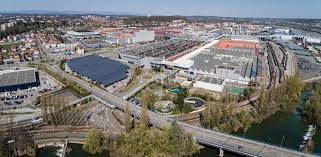
\includegraphics[width=0.75\textwidth]{images_pfe/stellantis.jpg}
  \caption{Sochaux Plant of Stellantis.}
  \label{fig:sochaux_plant}
\end{figure}

\FloatBarrier

% ═════════════════════════════════════════════════════════════
\section{\textcolor[HTML]{0066CC}{Organizational Structure and Interfaces}}
\label{sec:org-structure}
% ═════════════════════════════════════════════════════════════

\subsection*{\textcolor[HTML]{003D99}{2.2.1 Mechatronics Engineering: Mission and Scope}}

The internship was performed within the \textbf{Mechatronics Engineering Department} of the Sochaux site. Mechatronics is the integrated engineering which need to join three domains:
{\setlength{\intextsep}{6pt}
\begin{figure}[H]
  \centering
  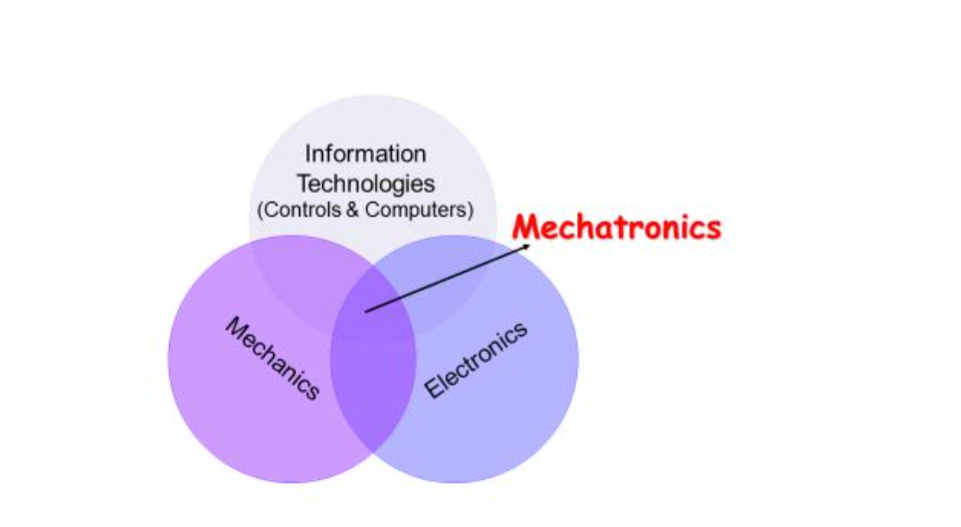
\includegraphics[width=0.75\textwidth]{images_pfe/mechatronics.png}
  \caption{Mechatronics Engineering Department Overview.}
  \label{fig:mechatronics_overview}
\end{figure}
}
\FloatBarrier
\vspace{-4pt}

It is the Mechatronics department that provides a high contribution to the systems evolution of the vehicle within the Stellantis program framework, making sure the three domains are working together providing advanced engineering system solutions for the automotive world. 
The department, together with System Engineering, Component Engineering and Project Management, guarantees the execution of all schedule and Technology Readiness levels deliverables (Gates 1, 2, 3 gates).
\vspace{0.3cm}

\subsection*{\textcolor[HTML]{003D99}{2.2.2 Key Stakeholder Roles in Governance}}

There are 4 main functions involved in Sochaux management, each has a precise task to be carried out within the component validation and gate release process. Those can be summarised as below:
\vspace{0.3cm}


\begin{table}[H]
\centering
\small
\setlength{\tabcolsep}{8pt}
\renewcommand{\arraystretch}{2.2}
\caption{Governance roles and responsibilities at Sochaux Mechatronics.}
\label{tab:governance-roles}
\begin{tabularx}{\textwidth}{|>{\raggedright\arraybackslash}X|>{\raggedright\arraybackslash}X|>{\raggedright\arraybackslash}X|}
\hline
\cellcolor[HTML]{E6F2FF}\textcolor[HTML]{003D99}{\textbf{Role}} & \cellcolor[HTML]{E6F2FF}\textcolor[HTML]{333333}{\textbf{Responsibilities}} & \cellcolor[HTML]{E6F2FF}\textcolor[HTML]{006600}{\textbf{Interactions \& Data Sources}} \\
\hline
\textbf{DL}\newline(Design Leader) & Technical ownership, Specification definition, PM coordination & Who-is-Who Excel entry, specification delivery, blocker escalation to PM \\
\hline
\textbf{DRE}\newline(Design Review Engineer) & Design review execution, Compliance verification, Gate readiness assessment & Specification review, gate criteria validation, documentation flagging \\
\hline
\textbf{CTE}\newline(Chief Technical Expert) & Multi-component support, Standards guidance, Conflict arbitration & On-demand technical advice, standards compliance, DL--DRE escalation point \\
\hline
\textbf{SSTL}\newline(Supplier Lead) & Supplier interface, Deliverable validation, Escalation path & Supplier communication, documentation validation, blocker escalation \\
\hline
\end{tabularx}
\end{table}

\vspace{0.2cm}


\noindent\textbf{Decision and Escalation Pathways:}

\vspace{0.3cm}

\fbox{\begin{minipage}{0.92\textwidth}

\small

\noindent\textcolor[HTML]{003D99}{\textbf{1. Routine Approval}} \quad $\Rightarrow$ DL \& DRE consensus required

\vspace{0.1cm}

\hspace{0.5cm} • Both actors aligned \quad $\Rightarrow$ \textcolor[HTML]{006600}{\textbf{Gate Progression}} 

\vspace{0.3cm}

\noindent\textcolor[HTML]{CC6600}{\textbf{2. Technical Disputes}} \quad $\Rightarrow$ CTE provides expert arbitration

\vspace{0.1cm}

\hspace{0.5cm} • If resolved \quad $\Rightarrow$ \textcolor[HTML]{006600}{\textbf{Decision}} 

\vspace{0.1cm}

\hspace{0.5cm} • If unresolved \quad $\Rightarrow$ \textcolor[HTML]{CC0000}{\textbf{Escalate to PM}}

\vspace{0.3cm}

\noindent\textcolor[HTML]{CC0000}{\textbf{3. Supplier Issues}} \quad $\Rightarrow$ SSTL manages supplier interface

\vspace{0.1cm}

\hspace{0.5cm} • If resolved \quad $\Rightarrow$ \textcolor[HTML]{006600}{\textbf{Decision}} 

\vspace{0.1cm}

\hspace{0.5cm} • If unresolved \quad $\Rightarrow$ \textcolor[HTML]{CC0000}{\textbf{Escalate to PM}}

\end{minipage}}

\FloatBarrier

% ═════════════════════════════════════════════════════════════
\section{\textcolor[HTML]{0066CC}{Department and Project Context}}
\label{sec:dept-context}
% ═════════════════════════════════════════════════════════════

\subsection*{\textcolor[HTML]{003D99}{2.3.1 Engineering Governance Processes}}

The governance in Sochaux is a cyclical approach (preparation/review/decision) related to milestones of the technical solution. These parts are governed by maturity gates (Gate 1, Gate 2, Gate 3), and involve creation, validation and approval of deliverables. This process includes teams of engineers (DL, DRE) and managers (PM, CTE), with well defined decisions taken, recorded and referenced.
\vspace{0.3cm}

\noindent\textbf{Governance Workflow:}

\begin{table}[!htbp]
\centering
\footnotesize
\setlength{\tabcolsep}{4pt}
\renewcommand{\arraystretch}{1.6}
\caption{Engineering Governance Workflow at Sochaux}
\begin{tabularx}{\textwidth}{|>{\raggedright\arraybackslash}p{1.55cm}|>{\raggedright\arraybackslash}p{1.5cm}|>{\raggedright\arraybackslash}p{2.05cm}|>{\raggedright\arraybackslash}p{2.1cm}|>{\raggedright\arraybackslash}p{1.8cm}|>{\raggedright\arraybackslash}p{1.8cm}|>{\raggedright\arraybackslash}p{1.85cm}|}
\hline
\textcolor[HTML]{003D99}{\textbf{Step}} & \textcolor[HTML]{003D99}{\textbf{Actor}} & \textcolor[HTML]{003D99}{\textbf{Action}} & \textcolor[HTML]{003D99}{\textbf{Inputs}} & \textcolor[HTML]{003D99}{\textbf{Outputs}} & \textcolor[HTML]{003D99}{\textbf{Decision}} & \textcolor[HTML]{003D99}{\textbf{Tools}} \\
\hline
Alignment & DL, PM & Discuss status, identify blockers & Project plan, task list & Current state & Proceed / escalate & Excel, SharePoint \\
\hline
Review & DRE & Inspect deliverables & Specifications, reports & Validation report & Accept / reject & SharePoint \\
\hline
Validation & DRE, DL & Check compliance & Deliverables & Compliance result & Approve / correct & SharePoint \\
\hline
Gate Decision & DL, DRE & Approve component status & Validation report & Approval & Gate pass / escalate & SharePoint, email \\
\hline
Escalation & CTE, PM & Resolve technical disputes & Issues & Solution & Resolution & Meetings, email \\
\hline
\end{tabularx}
\label{tab:governance-workflow}
\end{table}

\vspace{0.3cm}

\noindent\textbf{Process Flow:}

\vspace{0.3cm}

\noindent\fbox{\begin{minipage}{0.92\textwidth}
\centering
\small
\textcolor[HTML]{003D99}{\textbf{DL}} $\Rightarrow$ creates and uploads deliverables

\vspace{0.2cm}

\quad\quad\quad\quad\quad $\Downarrow$

\vspace{0.1cm}

\textcolor[HTML]{003D99}{\textbf{DRE}} $\Rightarrow$ reviews against gate requirements

\vspace{0.2cm}

\begin{tabular}{ll}
\quad\quad\quad\quad\quad $\Downarrow$ & \\
\end{tabular}

\vspace{0.1cm}

If \textcolor[HTML]{006600}{\textbf{validated}} $\Rightarrow$ \textcolor[HTML]{006600}{\textbf{gate progression approved}}

If \textcolor[HTML]{CC0000}{\textbf{issues}} $\Rightarrow$ \textcolor[HTML]{CC0000}{\textbf{DL applies corrections}}

If \textcolor[HTML]{FF6600}{\textbf{conflict}} $\Rightarrow$ \textcolor[HTML]{FF6600}{\textbf{escalation to CTE / PM}}

\end{minipage}}

\vspace{0.3cm}

\noindent\textbf{Gate Status Determination:}

Gate progression is tracked by looking at whether the document is available and is validated in SharePoint, not on a centralized system. The progression steps are as follows:
\vspace{0.3cm}

\begin{table}[H]
\centering
\small
\setlength{\tabcolsep}{8pt}
\renewcommand{\arraystretch}{2.2}
\caption{Gate Progression Requirements at Sochaux Mechatronics.}
\label{tab:gate-progression}
\begin{tabularx}{\textwidth}{|>{\raggedright\arraybackslash}X|>{\raggedright\arraybackslash}X|>{\raggedright\arraybackslash}X|}
\hline
\cellcolor[HTML]{E6F2FF}\textcolor[HTML]{003D99}{\textbf{Gate 1}} & \cellcolor[HTML]{E6F2FF}\textcolor[HTML]{003D99}{\textbf{Gate 2}} & \cellcolor[HTML]{E6F2FF}\textcolor[HTML]{003D99}{\textbf{Gate 3}} \\
\hline
Specification approved and uploaded & Design report completed + Design Review closed & Test reports + Compliance certificates available \\
\hline
\end{tabularx}
\end{table}

\vspace{0.2cm}

\noindent This is a document based system and, as such, is flexible; but care must be taken to monitor the system, as data can become disparate or inconsistent.

\vspace{0.3cm}

\noindent\textbf{Integration with LEON:}

Based on the requirements identified for this specific model of operational governance (manual sync, document correctness and decentralized data sources) there is a need for a system which will provide easy access to governance information and automate these requirements. A system capable of fulfilling these requirements (LEON) is described in the following sections.

\subsection*{\textcolor[HTML]{003D99}{2.3.2 Current Challenges in Governance Operations}}

Three persistent challenges constrain governance effectiveness at Sochaux:

\vspace{0.2cm}

\noindent\textbf{1. Information Fragmentation}

All the governance data (roles, status of gates, deliverables) are located in separated places: in an Excel spreadsheet stored on a SharePoint site, in a project portal database and in an e-mail sheet archives. If an engineer would like to know who is DRE for a given component, the following procedure should be performed: enter in project directory, search the right responsibility spreadsheet, locate the component, analyze the role columns. It could take from 10 seconds to one hour depending on the sheet condition.
\vspace{0.2cm}

\noindent\textbf{2. Data Inconsistency}

It is possible for a component to have different DLs or DREs on different Excel spreadsheets (example across projects, or at different times on the same project due to the changing of responsibility). If there is no single source of truth, the stakeholders have no means of knowing which data is the most current, and the teams sit around waiting for decision and approval of rework.
\vspace{0.2cm}

\noindent\textbf{3. Manual Coordination Overhead}

At each review / gate decision, this action is manually executed: collect data (check state of deliverable by person in charge, check for conformingness). As many projects running in parallel, and several elements within a project to manage, this overhead increases exponentially.
\FloatBarrier

% ═════════════════════════════════════════════════════════════
\section{\textcolor[HTML]{0066CC}{Internship Scope and Deliverables}}
\label{sec:internship-scope}
% ═════════════════════════════════════════════════════════════

\vspace{0.3cm}

\subsection*{\textcolor[HTML]{003D99}{2.4.1 Genesis of LEON: Addressing Governance Challenges}}

It is intended that \textbf{\textcolor[HTML]{0066CC}{LEON}} will be a governance support tool that will centralize a lot of consumed distributed governance information (e.g. roles, gate status) and be able to answer questions quickly. The tool will access existing storage location (SharePoint, Excel spreadsheet) and deliver information through natural language in no waiting for search.

\vspace{0.2cm}

\noindent\textbf{Scope and Intent:}

LEON is not intended as a replacement for governance process validation, gate decisions, or compliance checks. They are carried out by human stakeholders (DL, DRE, CTE, PM). LEON helps to share information and coordinate in order to help engineers do the actual technical decisions rather than information retrieval.
\vspace{0.2cm}

\noindent\textbf{Addressing the Challenges:}

\begin{table}[!htbp]
\centering
\small
\setlength{\tabcolsep}{8pt}
\renewcommand{\arraystretch}{1.8}
\caption{How LEON Addresses Governance Challenges}
\begin{tabularx}{\textwidth}{|>{\raggedright\arraybackslash}X|>{\raggedright\arraybackslash}X|}
\hline
\cellcolor[HTML]{E6F2FF}\textcolor[HTML]{003D99}{\textbf{Challenge}} & \cellcolor[HTML]{E6F2FF}\textcolor[HTML]{003D99}{\textbf{LEON Contribution}} \\
\hline
Information Fragmentation & Centralizes Who-is-Who and gate status data from distributed repositories into single queryable source \\
\hline
Data Inconsistency & Enforces single version of authority with audit trail; stakeholders access same data \\
\hline
Manual Coordination Overhead & Enables instant response to routine queries (role lookup, gate status) without manual search cycles \\
\hline
\end{tabularx}
\label{tab:leon-challenges}
\end{table}

The next chapter deals with the technical design and the prototype implementation of LEON to fulfill the requirements stated.
\FloatBarrier

Work on the LEON prototype was done in three parallel work packages analysis (of the system‘s requirements), implementation (on the hardware) and validation (using representative scenarios).
\vspace{0.5cm}

\subsection*{\textcolor[HTML]{003D99}{2.4.2 Work Package 1 (WP1): Requirements Elicitation and Specification}}

\noindent\textbf{Objective} : Identify and list recurring major governance questions as well as the technical requirements.

\vspace{0.2cm}

\noindent\textbf{Activities} : Conducted stakeholder (DLs, DREs, PMs) interviews to collect usual questions and blockers in their processes. Collecting essential functions such as knowledge Who-is-Who, gate status, document check. Documented constraints are roles of access, data compliance and usabilty.

\vspace{0.2cm}

\noindent\textbf{Deliverables} : Reporting of requirements specification, user scenario catalog, system context diagram.

\vspace{0.5cm}

\subsection*{\textcolor[HTML]{003D99}{2.4.3 Work Package 2 (WP2): System Design and Prototype Implementation}}

\noindent\textbf{Objective} : To develop and deploy a working prototype onto the Stellantis enterprise systems.

\vspace{0.2cm}

\noindent\textbf{Activities} : Designed a system architecture that meets the requirements using the available enterprise tools (conversation engine, workflow orchestration, integrate with SharePoint and Excel tools). Implemented system functionality (Who-is-Who in excel, Infer deliverable status based on sharepoint gates, role based access etc..). Configured SharePoint integration.

\vspace{0.2cm}

\noindent\textbf{Deliverables} : System architecture documents, implementation manual, deployment kit for prototype.

\vspace{0.5cm}

\subsection*{\textcolor[HTML]{003D99}{2.4.4 Work Package 3 (WP3): Evaluation and Scenario-Based Testing}}

\noindent\textbf{Objective} : Verification of operation and applicability for real world use.

\vspace{0.2cm}

\noindent\textbf{Activities} : Prototype has been implemented to simulate test environment considering normal governance use cases. Conducted functional tests with reference to user journeys, correctness check of role lookup and gate status inference, correctness check of access control enforcement.

\vspace{0.2cm}

\noindent\textbf{Deliverables} : Test report, performance assessment, security assessment, feedback from stakeholders, recommendation to production



% ═════════════════════════════════════════════════════════════
\section{\textcolor[HTML]{0066CC}{Problem Definition \& Objectives}}
\label{sec:problem-objectives}
% ═════════════════════════════════════════════════════════════

\subsection{\textcolor[HTML]{003D99}{Problem Definition}}
\label{subsec:problem-def}

\subsubsection*{\textcolor[HTML]{003D99}{Central Problem Statement}}

The Mechatronics department at Sochaux faces a permanent operational difficulty: \textbf{the governance information required to answer common engineering questions (role, state of the gate, condition of compliance ...) is distributed in various systems and storage spaces, causing coordination effort and incoherence of the governance solution.}.

\vspace{0.3cm}

\subsubsection*{\textcolor[HTML]{003D99}{Root Causes and Symptoms}}

Team members (DL, DRE, CTE, SSTL) expect rapid and specific answers regarding normal governance problems. Currently, it is necessary to do a long (manual) search in the infrastructure:

\vspace{0.2cm}

\begin{table}[!htbp]
\centering
\small
\setlength{\tabcolsep}{8pt}
\renewcommand{\arraystretch}{2.1}
\caption{Governance Information Needs and Current Barriers}
\begin{tabularx}{\textwidth}{|>{\raggedright\arraybackslash}X|>{\raggedright\arraybackslash}X|>{\raggedright\arraybackslash}X|}
\hline
\cellcolor[HTML]{E6F2FF}\textcolor[HTML]{003D99}{\textbf{Question Needed}} & \cellcolor[HTML]{E6F2FF}\textcolor[HTML]{003D99}{\textbf{Current Process}} & \cellcolor[HTML]{E6F2FF}\textcolor[HTML]{003D99}{\textbf{Barriers}} \\
\hline
``Who is responsible for component X in role Y?'' & Manual Excel search, cross-reference sheets & Multiple sources, outdated data \\
\hline
``What is gate status of component Z?'' & Check SharePoint folder, infer from documents & No centralized metadata \\
\hline
``Is documentation meeting gate requirements?'' & Engage expert for manual review & Delays, inconsistent interpretation \\
\hline
\end{tabularx}
\label{tab:information-needs}
\end{table}

\vspace{0.3cm}

\subsubsection*{\textcolor[HTML]{003D99}{LEON's Value Proposition}}

\textbf{\textcolor[HTML]{0066CC}{LEON}} is proposed as a unified governance agent that:

\begin{itemize}
  \item \textbf{Centralizes access} to the right governance information (roles, gates, templates, rules on compliance).
  \item \textbf{Automates routine queries} to take some part of coordination load away, as well as shorten response time.
  \item \textbf{Enforces consistency} through centralized control and use of role-based access.
  \item \textbf{Provides traceability} of all governance decisions and actions to the extent required to comply with an audit.
  \item \textbf{Preserves human oversight} by including human validation and an escalation mechanism within it for critical decisions.
\end{itemize}

\FloatBarrier

\subsection{\textcolor[HTML]{003D99}{System Constraints and Design Drivers}}
\label{subsec:constraints}

\textbf{\textcolor[HTML]{0066CC}{LEON}} is implemented under certain enterprise constraints which is typical for the majority of industrial engineering type work environment. Due to that internal repositories must be made available to the users by role in order to avoid that governance data is exposed to everybody. Confidentiality constraints also prevent unreserved access to the information details which is contained in disclosed tools. The accountability of all access can support system auditing and the existence of LEON as a support rather than decision support can be regarded as being advantageous for the human decision makers.

\FloatBarrier

\subsection{\textcolor[HTML]{003D99}{Objectives and Success Criteria}}
\label{subsec:objectives}

\subsubsection*{\textbf{\textcolor[HTML]{0066CC}{Primary Objective}}}

Design and deliver a prototype governance agent that centralizes access to authoritative governance information and enables team members to obtain accurate answers to recurring governance questions through natural language conversation, while maintaining strict role-based access control and auditability.

\vspace{0.5cm}

\subsubsection*{\textbf{\textcolor[HTML]{0066CC}{Measurable Sub-Objectives and Success Criteria}}}

\begin{enumerate}
  
  \item \textbf{\textcolor[HTML]{003D99}{SO1 -- Who-is-Who Lookup:}} Users must be able to query: ``Who is responsible for component X in role Y (DL/DRE/CTE/SSTL)?'' 
  \\\\
  \textbf{Success criterion:} System retrieve authoritative responsible persons from centralized governance dataset within a reasonable time frame (< 5s).
  
  \vspace{0.3cm}
  
  \item \textbf{\textcolor[HTML]{003D99}{SO2 -- Gate Status Support:}} Support requests for component maturity in the context of Gate 1, Gate 2, and Gate 3 readiness through Mechatronics governance.
  \\\\
  \textbf{Success criterion:} The system returns the correct Gate progress state based on documented available information.
  
  \vspace{0.3cm}
  
  \item \textbf{\textcolor[HTML]{003D99}{SO3 -- Document Management Support:}} Provide and maintain authorized repository structure for submission of governance documents (specification / test report / evidence of compliance) and apply the relevant metadata and access control.
  \\\\
  \textbf{Success criterion:} The system checks constraints in user permissions and confidentiality; the files which are stored in the system include full metadata (who uploaded it and when, user‘s access level to the document and which system‘s component makes use of this file).
  
  \vspace{0.3cm}
  
  \item \textbf{\textcolor[HTML]{003D99}{SO4 -- Communication Support:}} Assists users to create and send emails related to the governance (status notification, reporting an anomaly) in an appropriate format and to the correct address (by using message templates and recipient resolution templates)
  \\\\
  \textbf{Success criterion:} System correctly resolves receivers from directory, allows preview and tracks all messages, keeps audit trail for communications.
  \vspace{0.3cm}
  
  \item \textbf{\textcolor[HTML]{003D99}{SO5 -- SpecValidator (Compliance Checking):}} Enable the ability to validate a certain technical specification in a systematic, reproducible manner resulting in a complete set of reports for the expert analysis.
  \\\\
  \textbf{Success criterion:} The validation engine can generate multiple rule sets appropriately used, suitably raise violations with comprehensible explanations, and yield the validated outcomes that will be employed to the assurance audit without modifying original specifications.
  
\end{enumerate}


% ═════════════════════════════════════════════════════════════════════════════
% CHAPTER 3: État de l'Art (State of the Art)
% Restructured for proper thesis hierarchy
% Original content preserved between markers - DO NOT EDIT
% ═════════════════════════════════════════════════════════════════════════════

\chapter{State of the Art and Technical Foundations}
\label{chap:state-of-art}

% ═════════════════════════════════════════════════════════════════════════════
\section{\textcolor[HTML]{0066CC}{Artificial Intelligence}}
\label{sec:ai-basics}
% ═════════════════════════════════════════════════════════════════════════════

\subsection*{\textcolor[HTML]{003D99}{Overview and Historical Development}}

Artificial intelligence is a field of computer science which deals with the designing of intelligent systems, capable of performing human like tasks using algorithms which are developed and built upon in a computational framework. Systems with high enough capability can be regarded as intelligent to do human traditional tasks such as natural language understanding.
\begin{figure}[!htbp]
  \centering
  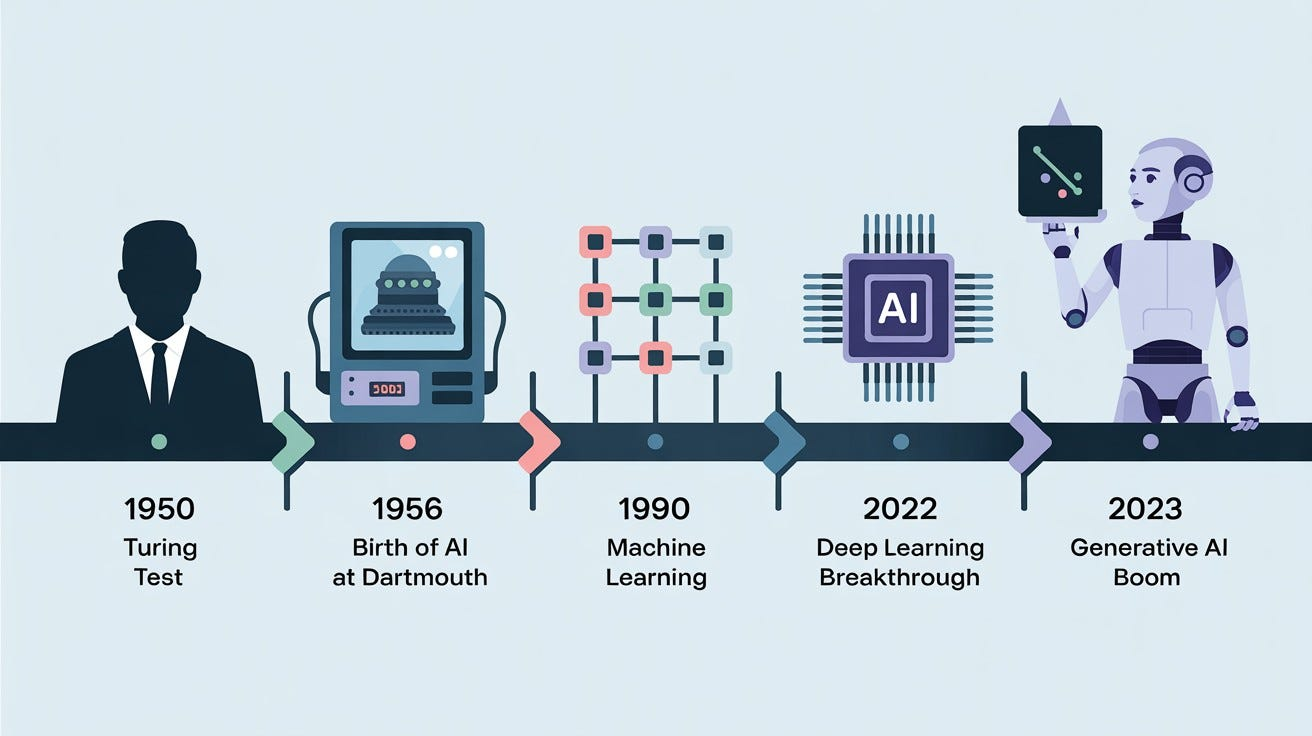
\includegraphics[width=0.75\textwidth]{images_pfe/history AI.jpg}
  \caption{Historical development of Artificial Intelligence.}
  \label{fig:history_ai}
\end{figure}
The specific term of artificial intelligence was first uttered as far back as 1956 by John McCarthy in his proposal for the Dartmouth Summer Research Project on Artificial Intelligence. AI has since progressed in phases, beginning with the symbolic and then experiencing a fall in popularity called an AI winter. Modern techniques have evolved in the form of deep learning, inspired by artificial neural networks.

\subsection*{\textcolor[HTML]{003D99}{Key Methodologies}}

To better understand this discipline, it is useful to distinguish several key authorities:

\noindent\textbf{Symbolic approaches:} In this domain, symbolic methodologies have a special advantage because of their ability to handle explicit knowledge. They are used for formalizing the rules of dialogue of a language (for example, in systems that have a natural language interface), and for implementing rule-based systems.

\noindent\textbf{Machine learning} allowing computers to acquire knowledge automatically from data and is also an important element to customize the Chatbots based on the users.

\noindent\textbf{The statistical approach} is more linked to the underlying theory because it attempts to make the uncertainty explicit by using probabilistic theory and is a statistical implications. It does this by representing uncertainty through probabilistic and statistical methods such as probability theory and Bayesian estimation.

\noindent\textbf{Artificial neural networks,} which form the basis of deep learning. One way to motivate neural networks is by the fact that the mechanisms involved are biologically analogous to human brain (Hertz et al., 1991, Domingos 2012). The methods developed are powerful for generate text and fused multimedia data.

\subsection*{\textcolor[HTML]{003D99}{Current Applications and Impact}}

In recent times, the uses of AI are vast and expanding. Speech recognition, computer vision, and recommenders systems are just some examples where AI are used widely. The combination of big data, greater processing power, and newalgorithmsare among the important reasons why artificial intelligence is getting popular recently.
\begin{figure}[!htbp]
  \centering
  
\includegraphics[width=0.75\textwidth]{images_pfe/AI use.png}
  \caption{Current applications and impact of Artificial Intelligence.}
  \label{fig:ai_uses}
\end{figure}
\FloatBarrier

% ═════════════════════════════════════════════════════════════════════════════
\section{\textcolor[HTML]{0066CC}{Generative Artificial Intelligence}}
\label{sec:generative-ai}
% ═════════════════════════════════════════════════════════════════════════════

\subsection*{\textcolor[HTML]{003D99}{Definition and Core Concepts}}

Generative AI employs all methods and models that generate original content text, images, music, audio, video, or other digital media in response to a prompt or to learn an AI lean an attention-based mechanism used primarily to generate the output a specific task, such as predicting a future outcome, categorizing things or clarifying features. AI. The generative model differs from other IM models in that it needs to learn the overall distribution of the training data rather than just learning to classify patterns or characteristics and can use this knowledge to create entirely new outputs that would have never exist on its own.

\begin{figure}[!htbp]
  \centering
  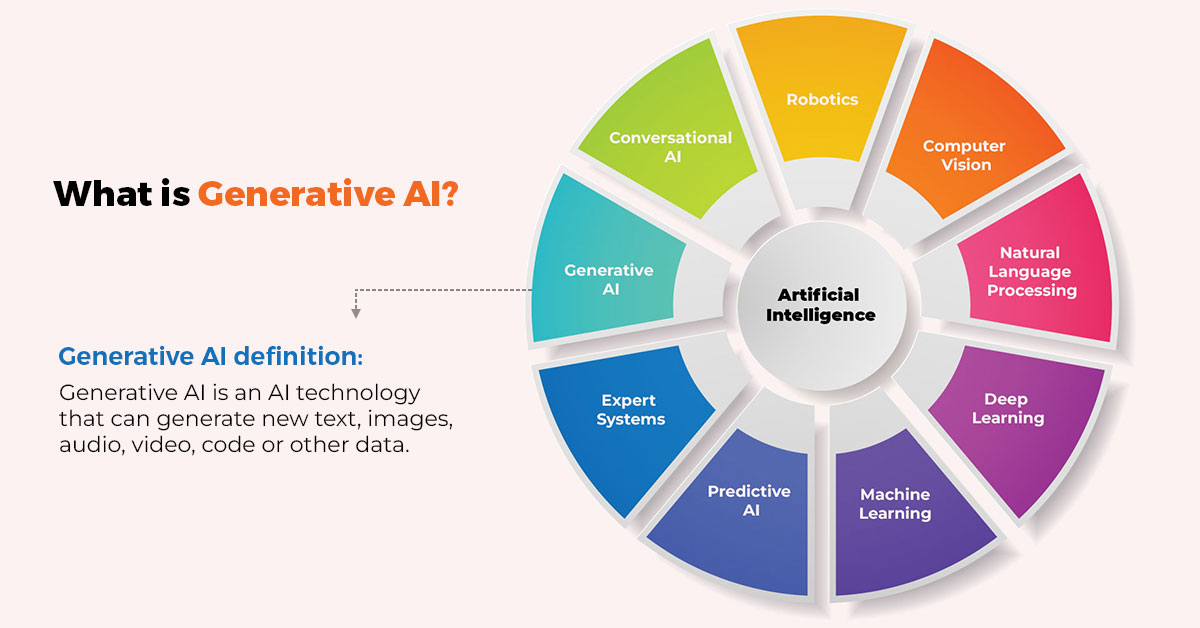
\includegraphics[width=0.75\textwidth]{images_pfe/GenAI.jpg}
  \caption{Concept of Generative Artificial Intelligence.}
  \label{fig:concept_generative_ai}
\end{figure}

\subsection*{\textcolor[HTML]{003D99}{Foundation Models: Concept and Role}}
\label{subsec:foundation-models}
The core of many different large scale or multimodal generative AI is a foundation model, typically either a large language model based chatbot like OpenAI's ChatGPT, Anthropic's Claude, or multimodal generator models for images, text-to-image generators for example. As given a foundation model is a model trained on broad data at scale to solve many tasks (using self-supervised learning and can be adapted to a wide range of downstream tasks.

\begin{figure}[!htbp]
  \centering
  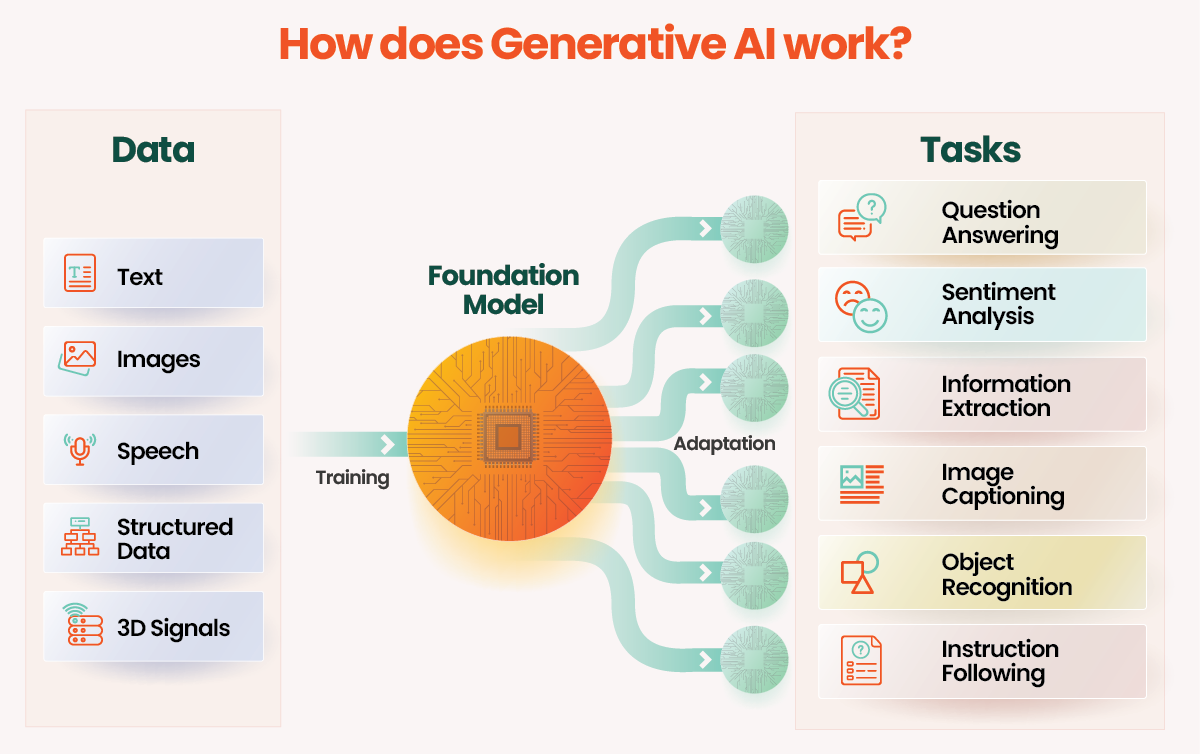
\includegraphics[width=0.75\textwidth]{images_pfe/foundation model.png}
  \caption{Concept of Foundation Models in Generative AI.}
  \label{fig:foundation_model}
\end{figure}

Self-supervised pretraining (SSP) for vision-language representations. In practice, large-scale pretraining, often referred to as pretraining, trains a model to produce representations for a wide variety of tasks based on diverse datasets, often using self-supervised or self-supervised learning methods.

Another important property of foundation models is that it is possible to adapt the same pre-trained model to multiple tasks without having to retrain from scratch each time; this can be accomplished by fine-tuning the model, instruction prompting, or through other techniques.

Furthermore, training foundational models requires significant amounts of resources and compute.

Another key reason for flexibility comes from the use of transfer learning, an area in which the foundation excel. The broad distribution of the knowledge used in pretraining is the core factor, because knowledge learned is often helpful for a variety of related downstream tasks.

\subsection*{\textcolor[HTML]{003D99}{Typology of Foundation Models}}
\label{subsec:foundation-typology}

There are a few main types of foundation models to consider: models designed for specific modalities (e.g., text, images, audio, video); models focused on specific capabilities (e.g., reasoning or generative). Foundation models are, in our framing, characterized by the usage of broad data at scale, such that they can adapt to many downstream tasks generic and broadly, often through selfsupervision.

\vspace{0.1cm}

\noindent\textcolor[HTML]{0066CC}{\textbf{Foundation Model Families and Their Applications:}}

\begin{table}[h!]
\centering
\caption{Typology of Foundation Models in Artificial Intelligence: Families, Descriptions, and Representative Examples}
\label{tab:foundation-typology}
\footnotesize
\setlength{\tabcolsep}{4pt}
\renewcommand{\arraystretch}{1.3}
\begin{tabularx}{\textwidth}{|>{\raggedright\arraybackslash}p{2.5cm}|>{\raggedright\arraybackslash}X|>{\raggedright\arraybackslash}X|}
\hline
\rowcolor[HTML]{0066CC}\color{white}\textbf{Foundation Model Family} & \color{white}\textbf{Description} & \color{white}\textbf{Representative Examples and Typical Use Cases} \\
\hline
\textcolor[HTML]{003366}{\textbf{Computer Vision Foundation Models}} & Models designed to analyze, interpret, and generate visual content (images and, in some cases, video) within a unified framework. & Florence: image description, visual question answering, object recognition, real-time video integration. \\
\hline
\textcolor[HTML]{003366}{\textbf{Unified Multimodal Foundation Models}} & Models capable of processing multiple input types (text, images, audio, video) and learning complex cross‑modal semantic relationships for richer contextual understanding. & GPT-4o (OpenAI), Gemini 2.0 (Google DeepMind), LLaMA 3.2 (Meta): advanced multimodal generation and understanding. \\
\hline
\textcolor[HTML]{003366}{\textbf{Large Language Models (LLMs) based on Transformers}} & Deep models built on Transformer architectures, specialized in understanding and generating natural language with strong contextual coherence. & Creation of ultra-realistic images, generation of synthetic data, enhancement of astronomical images, controlled deepfakes. \\
\hline
\textcolor[HTML]{003366}{\textbf{Generative Adversarial Networks (GANs)}} & Architectures composed of two neural networks trained in competition (generator vs. discriminator) to produce samples resembling training data. & GPT-3.5, GPT-4, Claude 3.5 (Anthropic), Mistral Large (open source), Grok (xAI): conversation, coding, complex reasoning. \\
\hline
\end{tabularx}
\end{table}

\FloatBarrier

\vspace{0.3cm}

In conclusion, these new models is a giant leap in AI field because they are capable of tackling vast number of unlabeled data and different task type, also they leverage multiple architecture styles, particularly transformers. Also, self-supervised learning seems to be a highly effective strategy for model training.\\
In order to perform this kind of task,  several computer vision models exist such as:  \textbf{Florence} (that understands the content of pictures),  \textbf{multimodal models (GPT-4,  Gemini 2.0)} that mix different types of data for their predictions,  \textbf{GANs (Good Automatic Networks)} which generate similar images, or \textbf{LLM (Long Large Models)} such as GPT-4 or Claude 3.5 which can predict natural text.\\

\subsection*{\textcolor[HTML]{003D99}{Traditional AI vs. Generative AI}}
\label{subsec:generative-vs-traditional}

GenAI systems are qualitatively different from earlier forms of \textbf{AI (e.g., Expert Systems, Machine Learning Classification/Regression models, etc.)}. Unlike prior applications of AI, which primarily made predictions on structured data and produced predictions within that structured domain (numbers, categories), GenAI is designed to produce new forms of unstructured data such as \textbf{text, images, audio, etc.} This new capability has been enabled by a particular architecture called the foundation model, particularly based on self-supervised learning using Transformer models trained on vast, diverse data.
\vspace{0.3cm}

\noindent\textcolor[HTML]{0066CC}{\textbf{Comparative Analysis: Traditional AI vs. Generative AI}}
\begin{table}[!htbp]
\centering
\caption{Comparison between Traditional AI and Generative AI}
\label{tab:traditional-vs-generative-ai}
\small
\begin{tabularx}{\textwidth}{|>{\raggedright\arraybackslash}p{2.5cm}|>{\raggedright\arraybackslash}X|>{\raggedright\arraybackslash}X|}
\hline
\rowcolor[HTML]{0066CC}\color{white}\textbf{Aspect} & \color{white}\textbf{Traditional AI} & \color{white}\textbf{Generative AI} \\
\hline
\textcolor[HTML]{003366}{\textbf{Type of content}} & Structured (tables, databases) & Unstructured (text, images, audio, video) \\
\hline
\textcolor[HTML]{003366}{\textbf{Models used}} & Task-specific models, often supervised & Foundation models (Transformers, LLMs) \\
\hline
\textcolor[HTML]{003366}{\textbf{Learning}} & Specific, labeled data & Large unlabeled datasets, self-supervised learning \\
\hline
\textcolor[HTML]{003366}{\textbf{Capabilities}} & Classification, prediction & Content generation, classification, prediction \\
\hline
\textcolor[HTML]{003366}{\textbf{Versatility}} & Limited to a specific task & Versatile, multi-task \\
\hline
\textcolor[HTML]{003366}{\textbf{Application examples}} & Object recognition, fraud detection & ChatGPT, DALL·E 2, Stable Diffusion, Bard \\
\hline
\textcolor[HTML]{003366}{\textbf{Limitations}} & High performance on a single task & Risk of hallucinations, lack of explainability \\
\hline
\end{tabularx}
\end{table}

\FloatBarrier

By comparison,  most of the \textbf{traditional AI} is narrowly defined in purpose,  and will typically perform analysis, classification, or prediction based on structured or semi-structured information.  The core advantage is its higher level of accuracy, since it is trained to perform a very specific function on a specific data set.

On one hand,  foundation models seem incredibly flexible, not only do they excel at most specific downstream tasks,  the same model appears adaptable to new tasks and domains, and capable of generating much more diverse and unexpected outputs.

On the other hand,  we note that generative AI do have some major drawbacks.  Firstly,  \textbf{hallucination phenomenon} which generates inaccurate, fake responses; lack of explainability, where the outputs and the reasoning are difficult to analyze; and optimization issues; where current models are not yet optimized enough for massive tabular data ingest and are not able to solve highly complicated problems.



In conclusion,  when traditional and generative AI are combined with human design,  powerful AI systems can be developed that are far greater than a system made only of traditionalAI, generative AI or human designers.
For example, If you have an AI enabled platform in place that has analyzed user behavior,  then generative AI could provide your platform with the capability to dynamically provide individualized user content.

\FloatBarrier

% ═════════════════════════════════════════════════════════════════════════════
\section{\textcolor[HTML]{0066CC}{Virtual Assistants and AI Agents}}
\label{sec:ai-agents}
% ═════════════════════════════════════════════════════════════════════════════

\subsection*{\textcolor[HTML]{003D99}{Definition and Core Capabilities}}

The recent advancements in natural language processing and machine learning have led to virtual assistants and AI agents that are a part of current human-computer interaction. Autonomousintelligentagents understand the intentions of the user and are able to achieve the user's goals with minimal user intervention. An (AI) Agent is a computer program or system that perceives its environment, reasons about available information and takes actions to achieve designated goals.
\begin{figure}[!htbp]
  \centering
  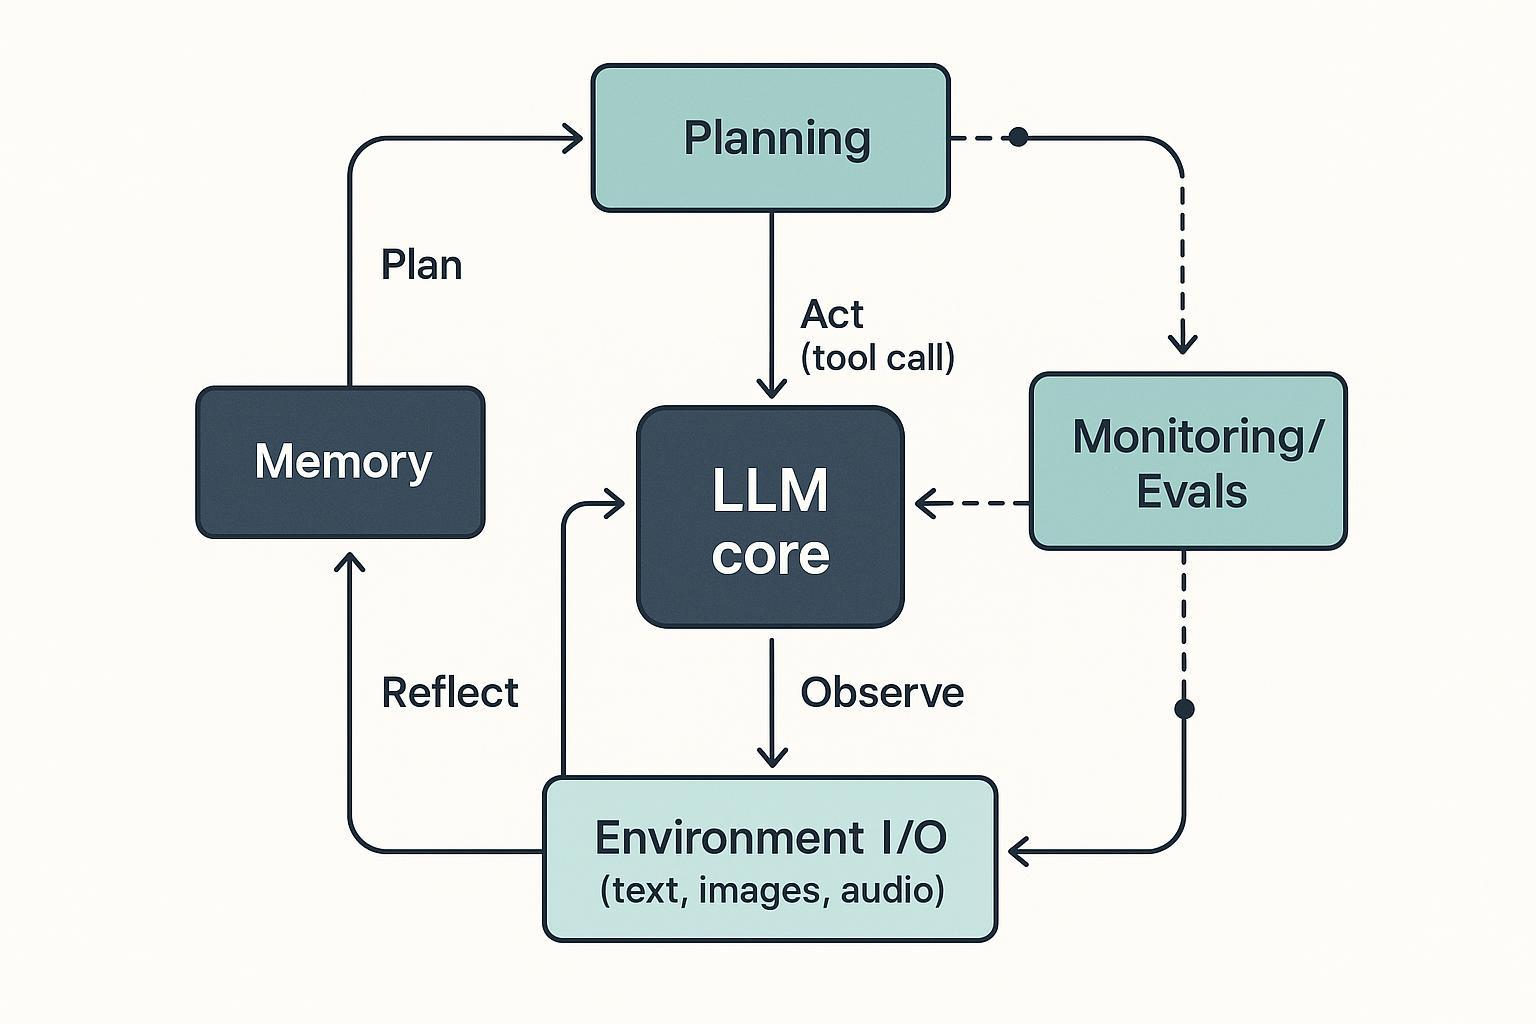
\includegraphics[width=0.75\textwidth]{images_pfe/concept Agent.jpg}
   \caption{Concept of AI Agents and Virtual Assistants.}
  \label{fig:concept_agent}
\end{figure}
\FloatBarrier

\vspace{0.2cm}

\noindent\textbf{Key Characteristics of Modern AI Agents:}

\vspace{0.2cm}

\noindent\textbf{(1) Natural Language Understanding:} Modern Agents are able to comprehend the verbal, written and also contextually-based utterances from a user in real-time. They would able to resolve and answer various queries such as to answer if I own X, to find Y, can you tell me something about Z, or can I do something on the PC.

\noindent\textbf{(2) Task Automation:} Represents complex sequences of actions, connect directly to different services (web applications, email client, local files, databases), or even simulate user activity on different applications without direct human interaction.

\noindent\textbf{(3) Contextual Awareness:} Effective agents ought to be able to manage their conversation context; this consists of keeping track of the history of the dialog, remembering facts about the world (a knowledge base), learning from past interactions and chasten their future behavior by making improvements.

\noindent\textbf{(4) Knowledge Integration:} Another crucial aspect of knowledge agent is its ability to aggregate data from a plurality of knowledge sources. So that knowledge agents are able to provide a comprehensive answer to queries posed by users.

\noindent\textbf{(5) Reasoning and Planning:} High end agents also know how to partition a task to several sub-tasks. Since, a task requested by the agent should be easily solvable by the robot. They will make an exhaustive search among possible ways to reach the objective. They are also able to reason about time constraints or material availability.

\FloatBarrier

% ═════════════════════════════════════════════════════════════════════════════
\section{\textcolor[HTML]{0066CC}{Large Language Models (LLMs)}}
\label{sec:llms}
% ═════════════════════════════════════════════════════════════════════════════

\subsection*{\textcolor[HTML]{003D99}{Overview and Core Architecture}}

All of the AI agents/virtual assistants that we have worked with are powered by a Large Language Model. An LLM is a type of deep neural network that has been trained on massive amounts of text data, such as book texts, websites, and other text sources. In LLM self-supervised learning, a model predicts continuations of a sequence of text, thereby allowing it to learn natural language patterns.
\begin{figure}[!htbp]
  \centering
  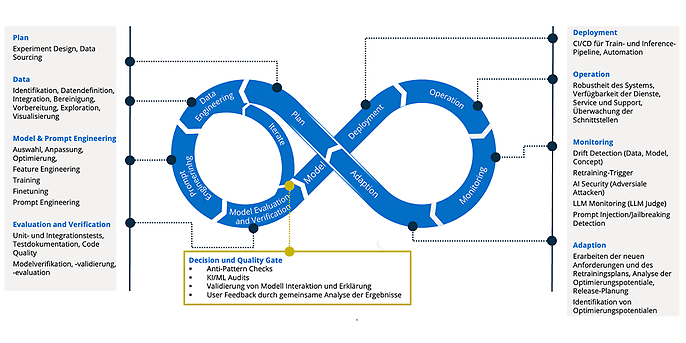
\includegraphics[width=0.75\textwidth]{images_pfe/LLM approach.png}
   \caption{Concept of Large Language Models (LLMs) and their architecture.}
  \label{fig:concept_llm}
\end{figure}
\FloatBarrier
\subsection*{\textcolor[HTML]{003D99}{Capabilities and Training Approaches}}

The task of these models is autoregressive language modeling, specifically the prediction of the next token in a sequence of text, given its previous tokens. The emergent capabilities that we see in the large-scale models are not directly encouraged by this training methodology, which is why the recent focus has been on instruction tuning (Fine-tuning large, pre-trained models on examples of following user instructions) and reinforcement learning from human preferences (RLHF) for the safer, more aligned and helpful models.

Because of the high flexibility of these systems, they can naturally be adapted to be foundation models that are particularly well-suited for an agent system, able to respond to a user's multifaceted queries whether as: a multi-turn conversational model; an instructed one, with clear reasoning why it came to a conclusion, or; prompted for structured data as output; and crucially, able to generalize between these tasks and adapt quickly to them with just small amounts of task specific fine-tuning via prompting techniques such as few shot learning.

\FloatBarrier

% ═════════════════════════════════════════════════════════════════════════════
\section{\textcolor[HTML]{0066CC}{Hallucination in Generative AI Systems}}
\label{sec:hallucination}
% ═════════════════════════════════════════════════════════════════════════════

\subsection*{\textcolor[HTML]{003D99}{Understanding Hallucination Phenomena}}

For LLM, given the enormous scale on which it's trained and its incredible skill, is capable of producing statements that are incredibly believable, but factually false. These falsehoods, known as hallucinations, occur for several possible reasons. In essence, hallucinatory responses arise as an accidental side effect of how these LLM's function. They don't remember pages from Wikipedia, instead they generate new text based on patterns of language that the model learned during its training phase. These patterns can cause an LLM to put together logical chains or claims, which are incorrect for the topic they're trained on.
\begin{figure}[!htbp]
  \centering
  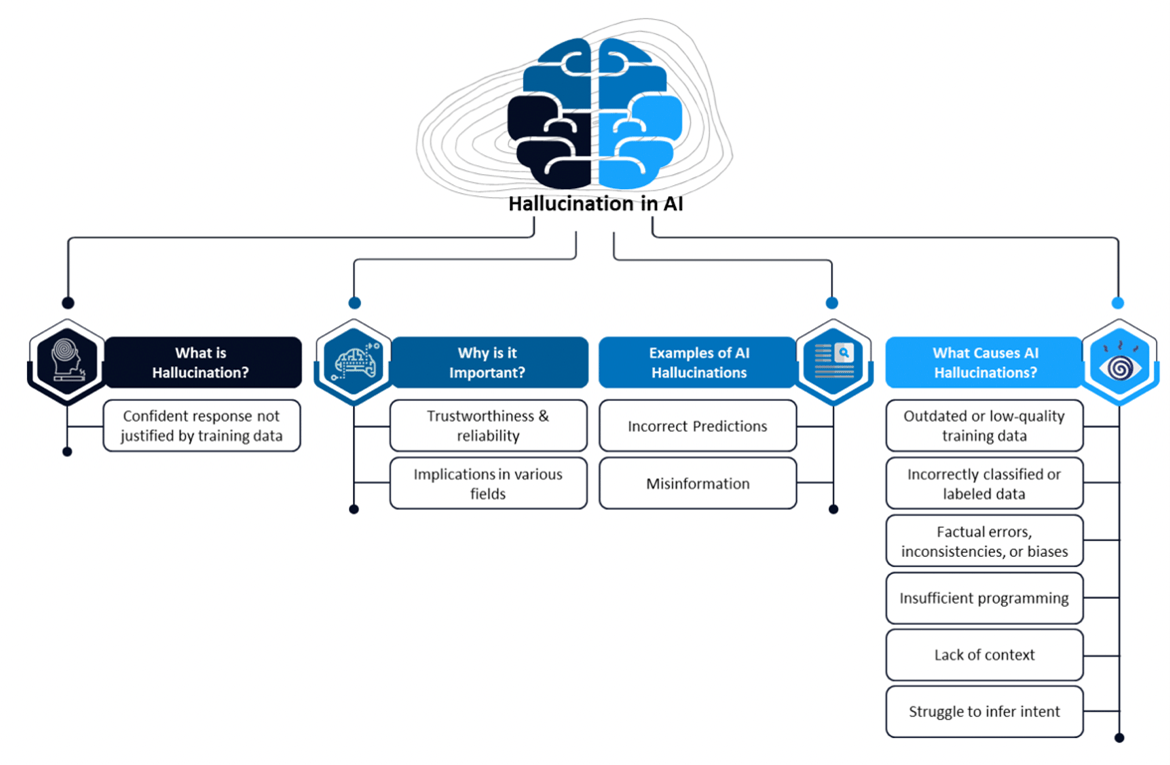
\includegraphics[width=0.75\textwidth]{images_pfe/AI hallucination.png}
   \caption{Concept of Hallucination in Generative AI Systems.}
  \label{fig:concept_hallucination}
\end{figure}
\FloatBarrier
\vspace{0.2cm}

\noindent\textbf{Sources and Types of Hallucination:}

\vspace{0.2cm}

\noindent\textbf{Factual Hallucination:} The model generates false facts that are inconsistent with any known factual knowledge.

\noindent\textbf{Logical Hallucination:} The model produces reasonable-looking reasoning chains that nonetheless contain logical fallacies or unwarranted assumptions.

\noindent\textbf{Context Hallucination:} Generating evidence for claims that are unsupported by, or are in contradiction to, the provided context. 

\noindent\textbf{Temporal Hallucination:} The model reported something that did not occur or who or what it reported is out of context using an incorrect time frame. 

\subsection*{\textcolor[HTML]{003D99}{Hallucination in Enterprise Applications}}

We posit that in the enterprise and governance applications in which LEON is applied, it is critical for the system to mitigate hallucination, especially in enterprise resource assignments, policy violations, invalid process recommendations, or wrong service invocation outcomes.

\FloatBarrier

% ══════════════════════Grounding and knowledge management ═══════════════════════════════════════════════════════
\section{\textcolor[HTML]{0066CC}{Grounding and Knowledge Management}}
\label{sec:grounding}
% ═════════════════════════════════════════════════════════════════════════════

\subsection*{\textcolor[HTML]{003D99}{Definition and Principles}}

\textbf{Grounding} refers to the process by which the outputs of an AI system are anchored, either textually, visually, or computationally, to sources of truth external to the system. The sources include various kinds of factual data, a writer's own documents, various kinds of current data, current systems, or trusted knowledge bases. With these components the agent is grounded and can be counted on to be traceable, accurate, and aware of the limits of its knowledge.

\vspace{0.2cm}

\noindent\textbf{Implementation Strategies for Grounding:}

\vspace{0.2cm}

\noindent\textbf{(1) Source Attribution:} The factual assertions made in an agent output should be traceable to either a source document, database, or API result.

\noindent\textbf{(2) Real-time Data Integration:} For a long lifespan agent, he can import much information from many authors. The agent may import that by its own or with the help of human.

\noindent\textbf{(3) Confidence Scoring:} Claims can be explicitly categorized as either passing through the system with high confidence, or inferred with a lower confidence.

\noindent\textbf{(4) Fallback Mechanisms:} If the agent is unsure about the current author or has not yet assigned an authority to the author, and if reliable authors are not the one the agent is currently addressing or would have addressed in his next step, fallback strategies must be used.

\FloatBarrier

% ═════════════════════════════════════════════════════════════════════════════
\section{\textcolor[HTML]{0066CC}{Retrieval-Augmented Generation (RAG)}}
\label{sec:rag}
% ═════════════════════════════════════════════════════════════════════════════

\subsection*{\textcolor[HTML]{003D99}{Framework and Architecture}}

\textbf{Retrieval-Augmented Generation (RAG)} is a powerful architectural pattern that attempts to fight hallucination and ground responses of LLMs by incorporating a Retrieval Component. The framework is straightforward; after receiving the user input, a Retriever extracts and returns a context document based on the query, and then the LLM uses thiscontext document and the query to produce an answer.
\begin{figure}[!htbp]
  \centering
  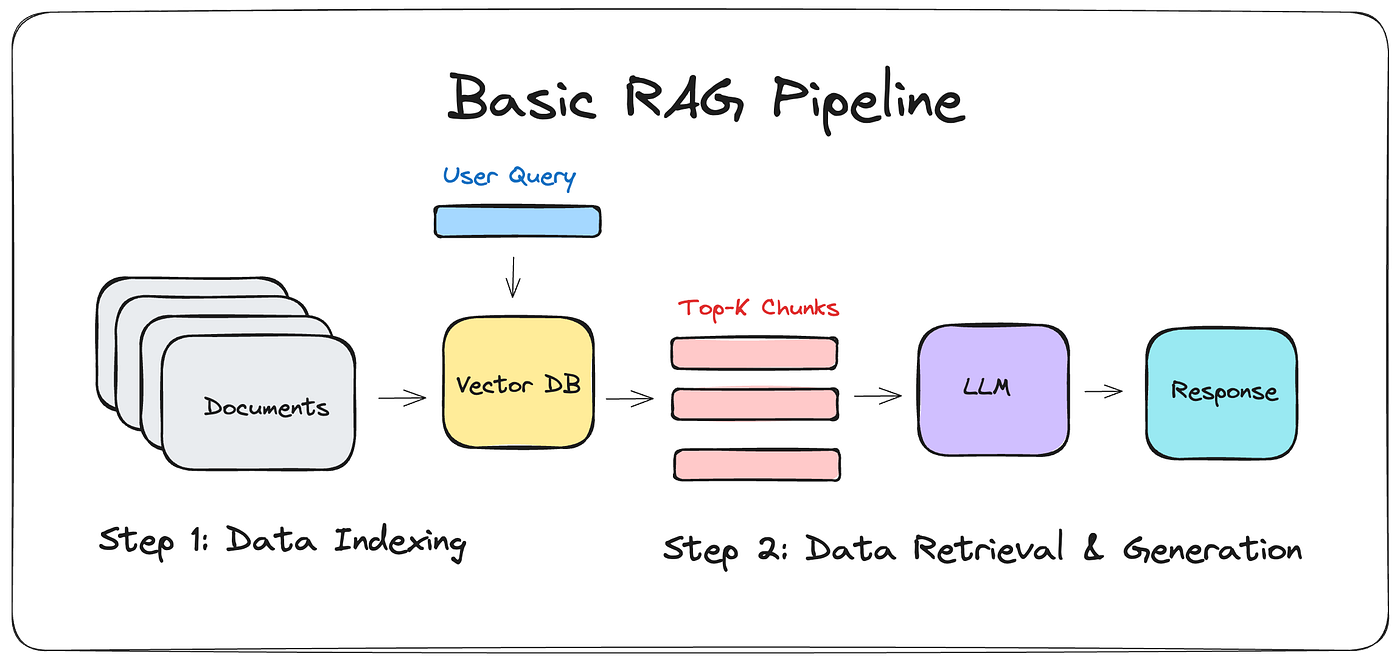
\includegraphics[width=0.75\textwidth]{images_pfe/RAG pipeline.png}
   \caption{Concept of Retrieval-Augmented Generation (RAG) pipeline.}
  \label{fig:concept_rag}
\end{figure}
\FloatBarrier
\vspace{0.2cm}

\noindent\textbf{RAG Architecture and Workflow:}

\vspace{0.2cm}

\noindent\textbf{(1) Query Encoding:} The step of taking the natural-language query input and turning it into a single number (called an embedding), such that all queries with the same semantic meaning are mapped to the same number.

\noindent\textbf{(2) Retrieval:} At retrieval, the user request is matched against a vector index of all the document/knowledge base entries, and content in contextually similar meaning is recovered.

\noindent\textbf{(3) Context Augmentation:} Factually relevant retrieved documents are directly concatenated to the front of the question text at inference time. The question itself remains in its original format, and no specific prompt formatting of context text is applied.

\noindent\textbf{(4) Grounded Generation:} The LLM generates a natural language answer to the query by conditioning on and grounding it within the retrieved context.

\noindent\textbf{(5) Source Citation:} A high quality RAG system must also provide accurate source citations. The system should have the ability to precisely identify all referential passages that contributed to the answer.

\subsection*{\textcolor[HTML]{003D99}{Key Advantages for Enterprise}}

\vspace{0.2cm}

\noindent\textbf{Accuracy and Hallucination Reduction:} RAG decreases inaccuracies and hallucinations by requiring the model to rely on provided resources rather than potentially spurious trends in the training data.

\noindent\textbf{Temporal Relevance:} This approach of dynamically pulling information makes them highly time-sensitive, enabling them to draw on up-to-date knowledge, as opposed to data collected at the time of training the LLM.

\noindent\textbf{Auditability and Compliance:} Each response returned would be easily traced and audited against sourced information. The responses will help satisfy enterprise governance, compliance and responsibility requirements.

\noindent\textbf{Knowledge Specialization:} While large language models are good general-purpose thinkers, they do not possess an organization's specific or domain specific knowledge. RAG alleviates the expense and difficulty of training a LLM on domain knowledge.

\noindent\textbf{Scalability:} LLMs are not able to grow with the scale of change in a business. The new knowledge can add to the index and LLMs do not need to be retrained.

Another significant aspect the agent needs, is the ability to use RAG for missioncritical operation. This may sound a bit dramatic for this case of study but this would be relevant in case of our governance agent, LEON. This is because in his case,  recommendations on how to use resources,  how to enforce a process or relevant technical document he refers to are based on external sources,  which he has to guarantee that he is actually taking the recommendations from these sources and not model hallucinations.

\FloatBarrier

% ═════════════════════════════════════════════════════════════════════════════
\section{\textcolor[HTML]{0066CC}{Orchestration: Conversation and Deterministic Automation}}
\label{sec:orchestration}
% ═════════════════════════════════════════════════════════════════════════════

\subsection*{\textcolor[HTML]{003D99}{Role in Enterprise AI Systems}}

\noindent\textbf{(1) Topic and Intent Classification:} The first step in orchestration is understanding what the user intends to accomplish. \textbf{Topics} represent broad functional areas (e.g., "resource allocation", "process compliance", "documentation validation"), while \textbf{intents} are specific actions within those domains (e.g., "who is available for task X", "check gate readiness", "validate specification"). Classification systems, often powered by LLMs or lightweight machine learning models, map user utterances to topics and intents, determining which automation workflow should be triggered.

\noindent\textbf{(2) Trigger Mechanisms:} A \textbf{trigger} is an event or condition that initiates an automated workflow. Triggers can be explicit (user-initiated via natural language: "Find team members qualified in embedded systems") or implicit (scheduled or event-driven: "Check all components' gate status daily"; "Notify when a specification update is posted"). Effective trigger design ensures that routine, repetitive tasks execute automatically while user-facing tasks respond immediately to requests.

\noindent\textbf{(3) Agent Workflows and Flows:} An \textbf{agent workflow} or \textbf{agent flow} is a structured sequence of deterministic steps that transform user intent into concrete outcomes. Unlike the probabilistic nature of LLM generation, workflows follow explicit branching logic, conditional rules, and predefined sequences. Workflows are composed of:

\vspace{0.1cm}


\noindent\indent • \textbf{Input Steps:} Retrieve user request parameters, context, and relevant domain information.

\noindent\indent • \textbf{Processing Steps:} Execute business logic—query databases, check compliance rules, validate constraints, apply transformations.

\noindent\indent • \textbf{Decision Points:} Branch based on conditions (if permission is granted, if availability exists, if specification is valid, etc.).

\noindent\indent • \textbf{Integration Steps:} Call external services, update systems, interact with APIs.

\noindent\indent • \textbf{Output Steps:} Format results, generate responses, provide citations and explanations.
\begin{figure}[!htbp]
  \centering
  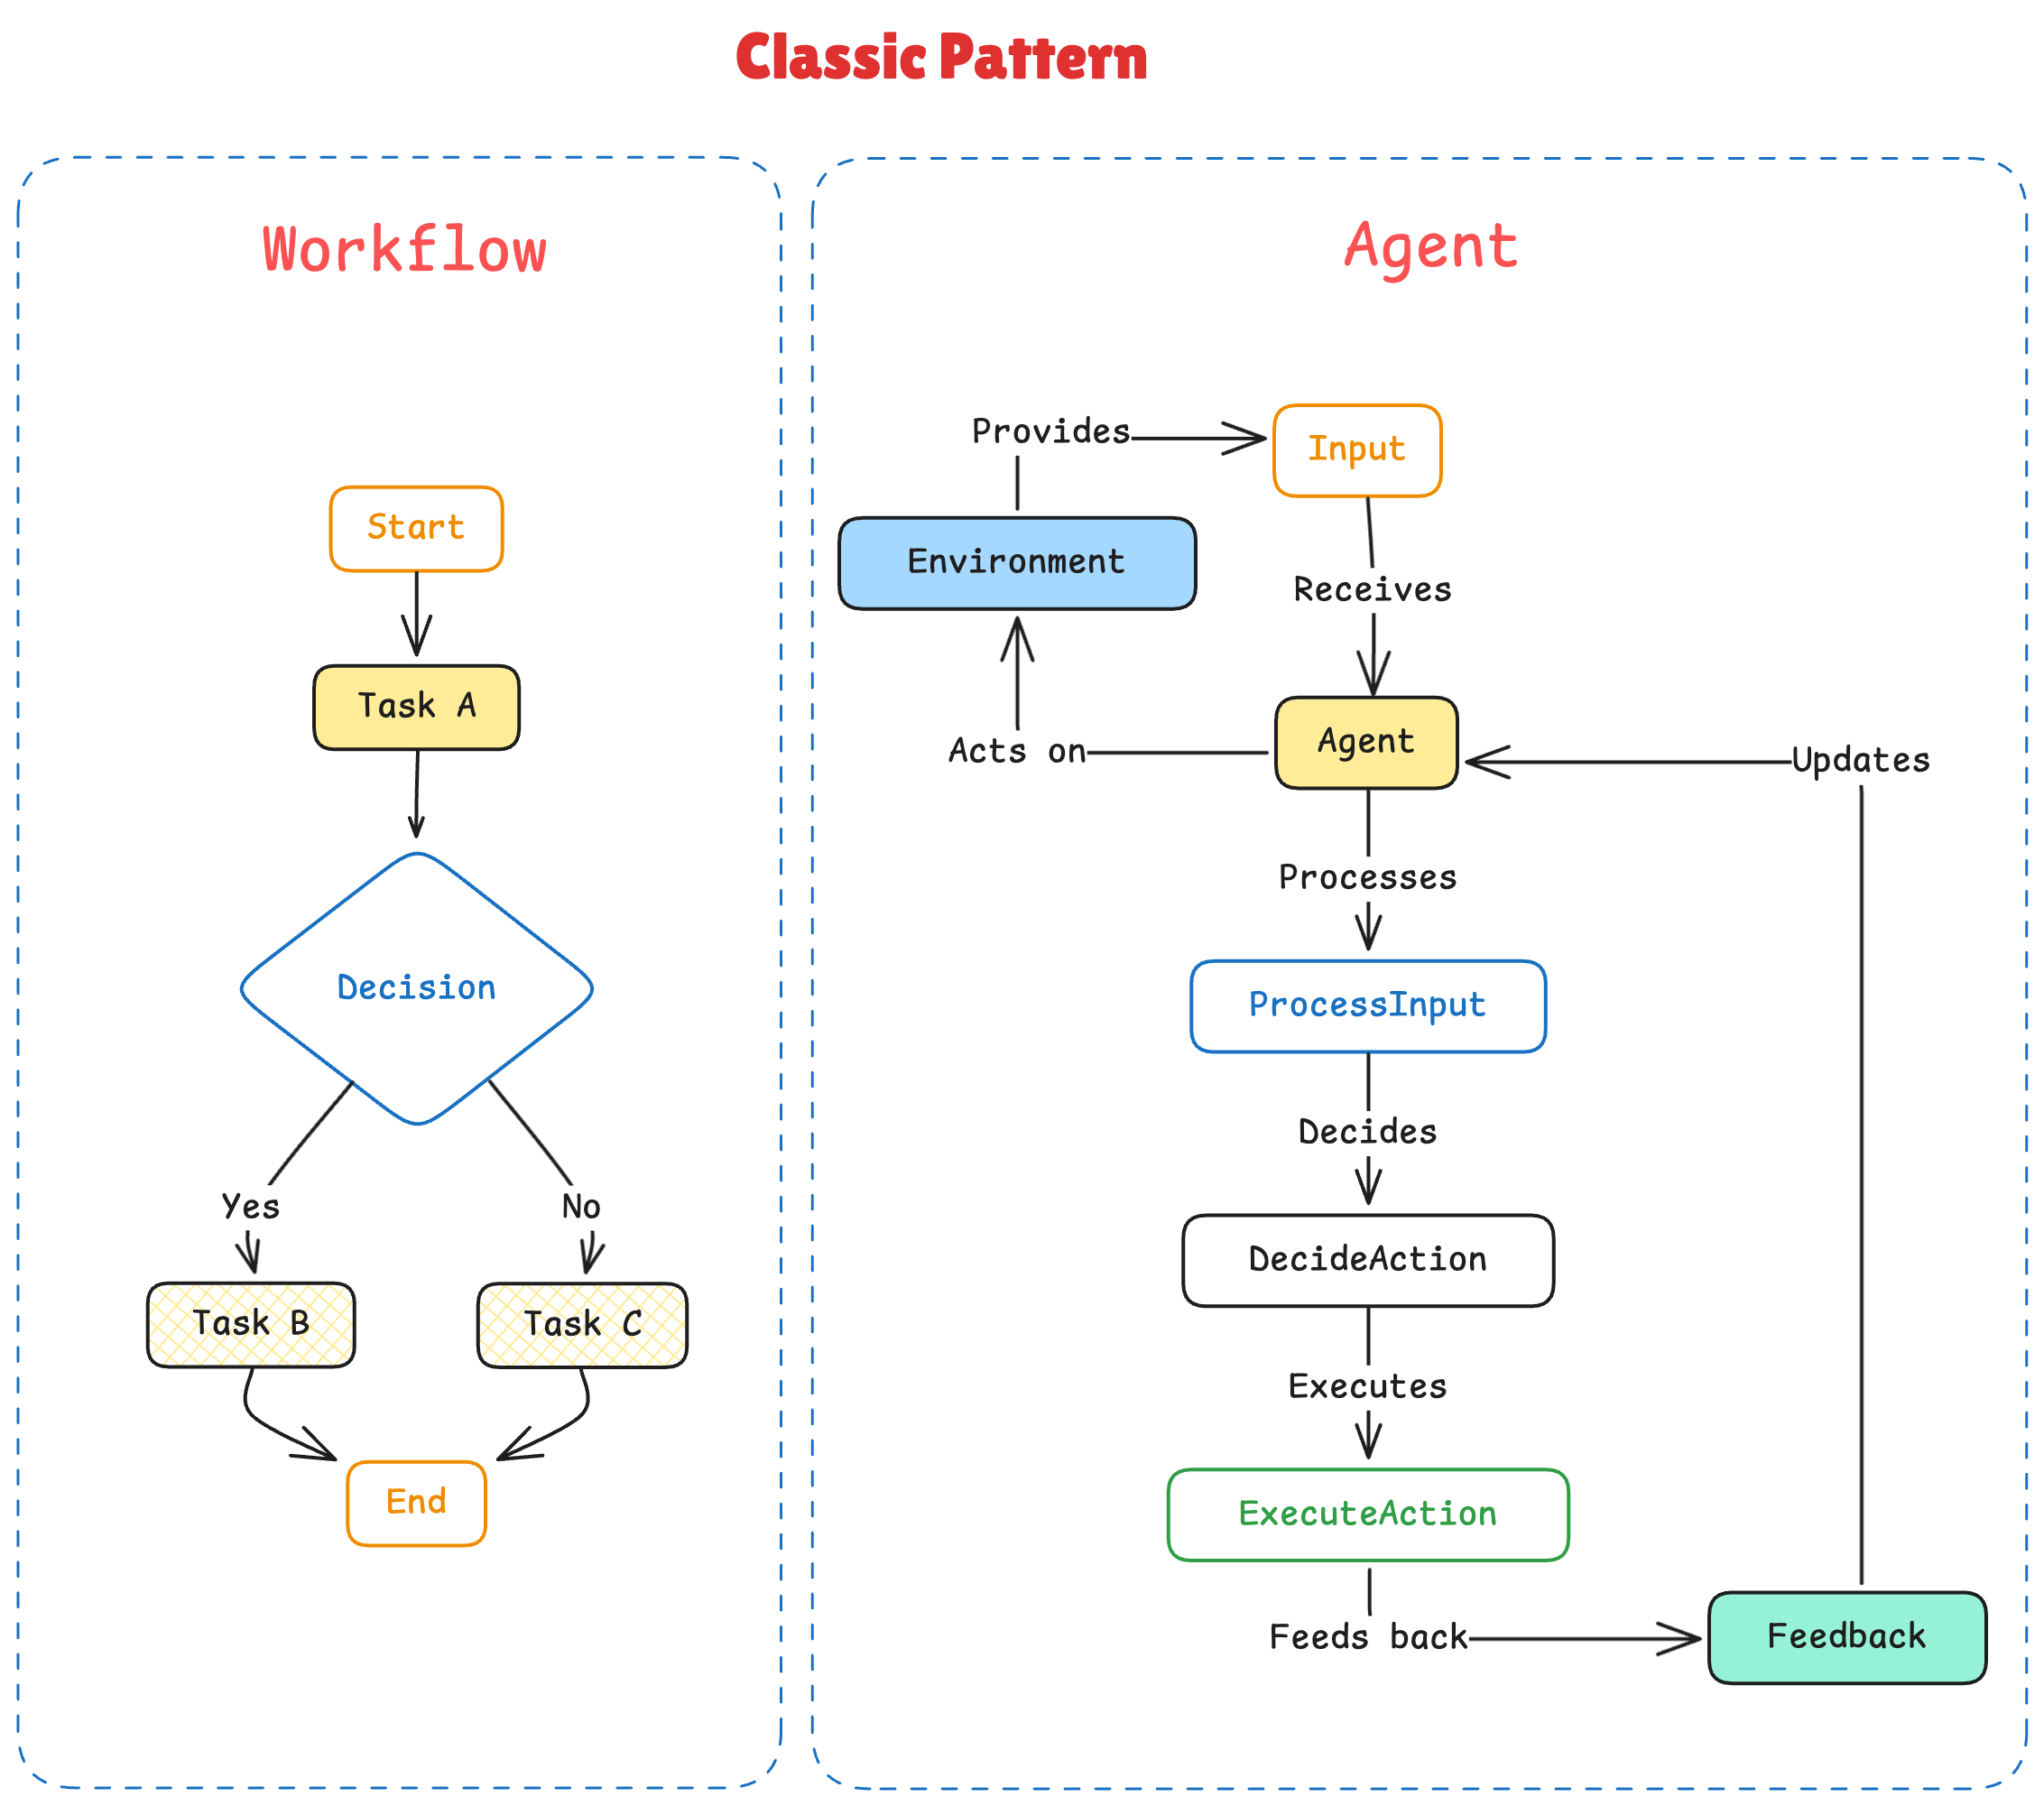
\includegraphics[width=0.75\textwidth]{images_pfe/agent workflow.png}
   \caption{Concept of Agent Workflows and Flows.}
  \label{fig:concept_agent_workflow}
\end{figure}
\FloatBarrier
\vspace{0.1cm}

\noindent\textbf{(4) API Connectors and Wrappers:} \textbf{API connectors} (or \textbf{wrappers}) are adapter modules that enable agent workflows to interact with external systems. A connector abstracts the complexity of underlying service APIs, providing a simplified interface for the agent. For example:

\vspace{0.1cm}

\noindent\indent • A \textbf{SharePoint connector} enables the agent to query document repositories, retrieve metadata, and check access permissions.

\noindent\indent • A \textbf{database connector} allows the agent to execute prepared queries against enterprise databases without exposing raw SQL or schema details.

\noindent\indent • A \textbf{email connector} enables the agent to compose and send messages on behalf of users, respecting approval workflows.

\noindent\indent • A \textbf{calendar connector} allows the agent to check availability, schedule meetings, and manage time-based events.

\vspace{0.1cm}

Connectors encapsulate error handling, authentication, rate limiting, and data transformation, providing the agent with reliable, safe interfaces to backend systems.

\subsection*{\textcolor[HTML]{003D99}{Power Automate and Repeatable Automation Logic}}

\vspace{0.2cm}

\textbf{Power Automate} (Microsoft's cloud-based workflow automation platform) exemplifies modern orchestration infrastructure. Power Automate "flows" are visual, low-code workflows that encode business logic in a format that is simultaneously human-readable (for business stakeholders) and machine-executable (for automation engines).
\begin{figure}[!htbp]
  \centering
  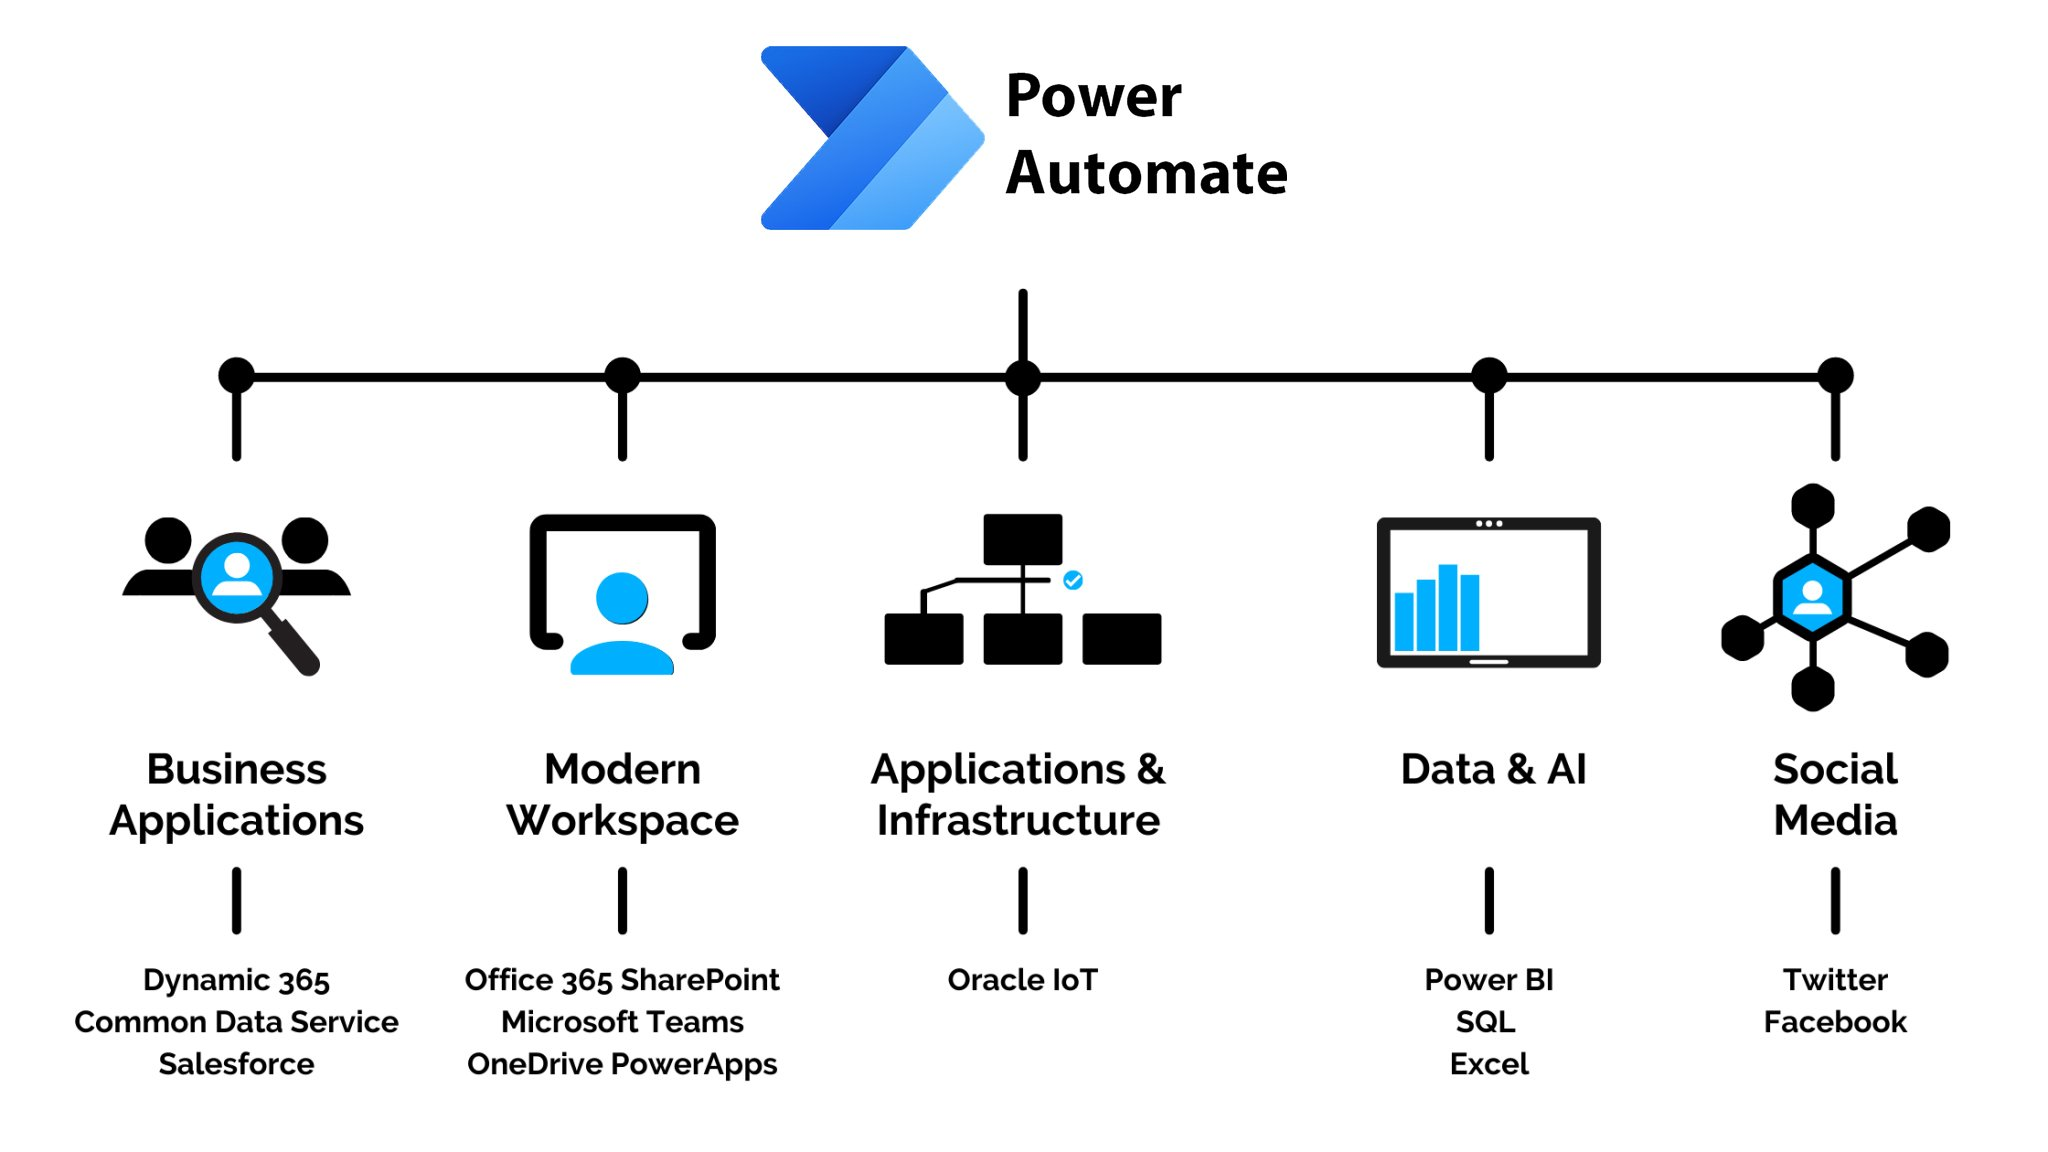
\includegraphics[width=0.75\textwidth]{images_pfe/power automate.jpg}
   \caption{Concept of Power Automate Flows.}
  \label{fig:concept_power_automate}
\end{figure}
\FloatBarrier
A Power Automate flow typically includes:

\vspace{0.2cm}

\noindent\textbf{Connectors:} Pre-built integrations with hundreds of enterprise systems (SharePoint, Exchange, SQL Server, Dynamics 365, Teams, Slack, Salesforce, etc.), eliminating the need to write custom integration code.

\noindent\textbf{Conditional Logic:} \texttt{If-Then-Else} branches, switch statements, and rule-based routing that make workflows deterministic and testable.

\noindent\textbf{Parallel Processing:} Simultaneous execution of independent steps (e.g., notify multiple stakeholders, check multiple systems) for efficiency.

\noindent\textbf{Approval Workflows:} Built-in approval steps that pause automation pending human review and decision, ensuring governance compliance.

\noindent\textbf{Data Transformation:} Tools for mapping, filtering, and transforming data between systems with different schemas or formats.

\noindent\textbf{Error Handling and Retry Logic:} Mechanisms to gracefully handle failures, retry failed steps, and notify administrators of issues.

\vspace{0.3cm}

By integrating LLM-based conversation with Power Automate flows, an agent becomes capable of both natural, flexible dialogue and reliable, repeatable automation. For instance:

\vspace{0.2cm}

\noindent\indent • User says: "Who is available to take the embedded software task for component X?" $\rightarrow$ Intent classified as "resource availability query" $\rightarrow$ Triggers a Power Automate flow that queries team database, checks calendars, filters by skill tags, and returns a ranked list grounded in authoritative sources.

\noindent\indent • User says: "Allocate Sarah to this task and notify the team" $\rightarrow$ Intent classified as "resource allocation" $\rightarrow$ Triggers an approval flow if required, updates the project management system, sends notifications via email/Teams, and logs the action for audit.

\noindent\indent • Scheduled trigger fires daily: Check all components' gate maturity status $\rightarrow$ Automatically queries engineering database, retrieves gate status from SharePoint portal, identifies components at risk of schedule slippage, and generates a summary report for governance meetings.

\subsection*{\textcolor[HTML]{003D99}{Orchestration in the Context of LEON}}

\vspace{0.2cm}

For the \textbf{LEON} governance agent, orchestration is essential to operationalize the agent's capabilities. Rather than relying solely on LLM outputs (which may hallucinate or miss domain constraints), LEON's workflows embed governance rules, access control policies, compliance checks, and approval gates. Conversations with LEON feel natural ("Who owns the electrical systems for the 3008?"), but behind the scenes, deterministic orchestration ensures accuracy (querying the authoritative organization database, checking user permissions, verifying data currency) and traceability (logging the query, the retrieved data sources, the response, and the timestamp).

This orchestration-driven approach transforms LEON from a conversational interface into a \textbf{trustworthy governance assistant}\textemdash one where accuracy is primarily achieved through system integration and rule enforcement rather than relying on the agent to "remember" domain knowledge or reason about complex policies.

% ═════════════════════════════════════════════════════════════════════════════
% End of Chapter 3: État de l'Art et Fondations Techniques
% ═════════════════════════════════════════════════════════════════════════════

% ═════════════════════════════════════════════════════════════════════════════
% Chapter 9: Design and Modeling of LEON
% ═════════════════════════════════════════════════════════════════════════════

\chapter{Design and Modeling of LEON}
\label{chap:design}

% ═════════════════════════════════════════════════════════════════════════════
\section{\textcolor[HTML]{0066CC}{Design Objectives}}
\label{sec:design-objectives}
% ═════════════════════════════════════════════════════════════════════════════

The design of LEON is grounded on four strategic pillars:

\begin{enumerate}
    \item \textcolor[HTML]{003D99}{\textbf{Conversational Flexibility}} : the conversational interface (Copilot Studio) must allow users to navigate freely among services (Who-is-Who, Gate tracking, Workload management) without imposing rigid flow, while guiding toward relevant actions.
    
    \item \textcolor[HTML]{003D99}{\textbf{Validation Determinism}} : the SpecValidator block must apply deterministic and reproducible validation rules, independent of the conversational layer, ensuring consistency in specification assessments.
    
    \item \textcolor[HTML]{003D99}{\textbf{Transparent Integration}} : LEON must integrate seamlessly with Stellantis's existing systems via enterprise connectors (directories, storage) and APIs, without disrupting current workflows.
    
    \item \textcolor[HTML]{003D99}{\textbf{Traceability and Audit}} : every action performed (search, modification, validation, notification) must be recorded to ensure compliance, auditability, and anomaly resolution. The system must maintain a complete history of decisions and modifications.
\end{enumerate}

% ═════════════════════════════════════════════════════════════════════════════
\section{\textcolor[HTML]{0066CC}{Functional View}}
\label{sec:design-functional-view}
% ═════════════════════════════════════════════════════════════════════════════
This section gives a description of the LEON system from the functional point of view. It gives details about services provided to the user and some system/actor interactions. The behavior of the system is described from user point of view, without technical constraints.
\subsection{Primary Services}

LEON delivers two categories of services:

\vspace{0.2cm}
\noindent\textcolor[HTML]{0066CC}{\textbf{A) Governance Services}}
Accessible via conversation, these services enable users to:
\begin{itemize}
    \item \textcolor[HTML]{003D99}{\textbf{Search for responsible party}} : query the Who-is-Who database to identify the person responsible for a component in a project.
    \item \textcolor[HTML]{003D99}{\textbf{Retrieve gate status}} : obtain current status (Gate 1, Gate 2, Gate 3, or other states defined by Stellantis).
    \item \textcolor[HTML]{003D99}{\textbf{Update responsibility assignments}} : modify responsibility assignments (subject to access control).
    \item \textcolor[HTML]{003D99}{\textbf{Manage workload}} : view and create/update task assignments and resource availability.
    \item \textcolor[HTML]{003D99}{\textbf{Send notifications}} : trigger communications (emails, reminders) to targeted stakeholders.
    \item \textcolor[HTML]{003D99}{\textbf{Upload deliverables}} : upload a file to the correct location associated with a gate.
\end{itemize}
\vspace{-4pt}

\vspace{0.2cm}
\noindent\textcolor[HTML]{0066CC}{\textbf{B) Validation Service}}
The SpecValidator service ensures that the technical specification complies with the engineering rules. It is invoked via conversational interface on user‘s request for the specification check.
\begin{itemize}
    \item \textcolor[HTML]{003D99}{\textbf{Specification templates and Rule files}} : The process of validation is relying on several structured inputs like references templates and set of rules that specify the content and quality of a specification then the service validates the document systematically.
    \item \textcolor[HTML]{003D99}{\textbf{Output}} :The validation output is provided as an organized report showing compliance results, non-compliance observations and proposed corrections. The report permits to display results to user and keeps document unchanged.
\end{itemize}
\vspace{-4pt}

\subsection*{\textcolor[HTML]{003D99}{Use Case Diagram}}

Figure~\ref{fig:leon-usecase-en} shows the use case diagram for the LEON system. This graph represents the relationship between the user and the system from a functional perspective.\\
The main users are engineer, project manager and administrators. The way they use the system is dependent on their level of control within the governance framework.
\vspace{-8pt}
\begin{figure}[H]
    \centering
    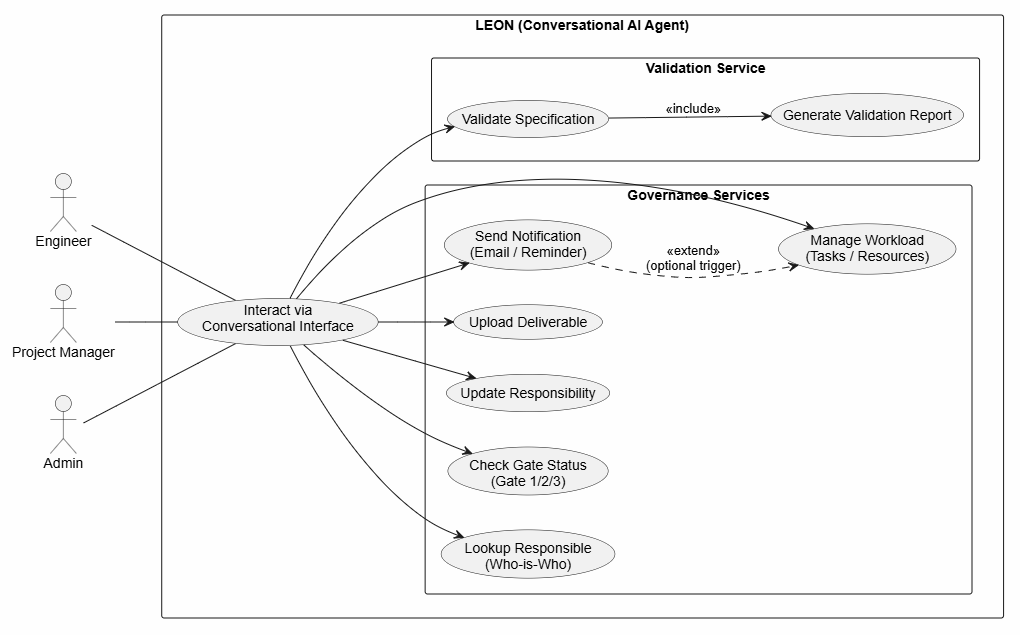
\includegraphics[width=0.85\textwidth]{images_pfe/use case diagram.png}
    \caption{LEON Use Case Diagram, high-level functional view}
    \label{fig:leon-usecase-en}
\end{figure}
\FloatBarrier
\vspace{-4pt}

These use cases are organized into two main groups, Services for Governance and Services for validation. The governance services covers governance related data (Who-is-Who, status of the Gate ownership) and data management (change of responsibility, document linking, document uploading) and services for Coordination (notifications, managing of training workflows). The validation services covers services for the SpecValidator module that checks technical specifications and generates technical reports about validation.\\
\vspace{0.5cm}
Centrally there is one conversational interface and therefore the services are accessed through one point of interaction, which makes switching between them simpler. In the diagram some connections are made between use cases; this is because of some inputs that need to be created (e.g. reports of validation) and some are dependent on others.\\
\vspace{0.5cm}
To conclude, in this functional view, LEON is perceived as a coherent layer among the set of governance functions and the set of distributed data.
% ═════════════════════════════════════════════════════════════════════════════
\section{\textcolor[HTML]{0066CC}{Structural View (Architecture)}}
\label{sec:design-structural-view}
% ═════════════════════════════════════════════════════════════════════════════

\subsection{Layered Architecture}

Under the layered architecture, this section will demonstrate the structural view of the LEON system in layered architecture form. It would be beneficial to separate the concern system of the user interface, the business, the data and the validation.

\vspace{0.2cm}
LEON is organized into four main logical layers:

\noindent\textcolor[HTML]{0066CC}{\textbf{1. Presentation / Conversation Layer}}
\begin{itemize}
    \item This represents the system entry layer. It provides the interaction with the user through a conversational user interface to enable stakeholders to access system services through a natural language.
    \item The described system is built on top of Copilot Studio that takes the users intentions and passes the request on to the corresponding service, furthermore it allows for conversational interactions.
    \item Role: Offers an interface that allows users to become abstract from applications, to interpret and validate their requests, and that is the interface to all appropriate services.
\end{itemize}

\noindent\textcolor[HTML]{0066CC}{\textbf{2. Orchestration and Business Logic Layer}}
\begin{itemize}
    \item This layer deals with performing all the operations related to the governance part. It receives commands from the Conversational Layer to be executed and then communicate with the interacting services.
    \item It implements governance functions (e.g. responsibility lookup, gate status retrieve, workload updates and message handling) using workflow features. It also handles the interface to external enterprise systems (e.g. directory services, document repositories and messaging).
    \item Role: Control the overall operations of the system and functionalities by defining the interaction flow among User, Data and Validation service
\end{itemize}

\noindent\textcolor[HTML]{0066CC}{\textbf{3. Processing / Validation Layer (Specialized)}}
\begin{itemize}
    \item This layer owns the processing units which are used to process domain-specific information. It is represented by the SpecValidator service in LEON, which checks the technical specifications.
    \item Validation is rule based and is executed using pre-defined templates from a repository which make validation a repeatable process. As validation is a singleton layer it doesn‘t depend on the conversational flow making validation activities deterministic.
    \item Role: Executes the task, separate validation logic from the UI.
\end{itemize}

\noindent\textcolor[HTML]{0066CC}{\textbf{4. Data and Configuration Layer}}
\begin{itemize}
    \item This layer contains the configuration data components as well as data components necessary for the system. Data components like the administration data sources (workloads, responsibilities etc) along with configuration components for validation exist in this layer.
    \item This Data is then archived in enterprise stores which might be document management systems or structured data stores. The system will also provide logging/auditing to achieve a clear trace of user/system interaction and to comply with standards.
    \item Role: provides long-term storage, configuration resources and ensures data integrity, consistency and traceability.
\end{itemize}

\subsection*{\textcolor[HTML]{003D99}{Architecture Diagram (Components)}}

\vspace{-8pt}
\begin{figure}[H]
    \centering
    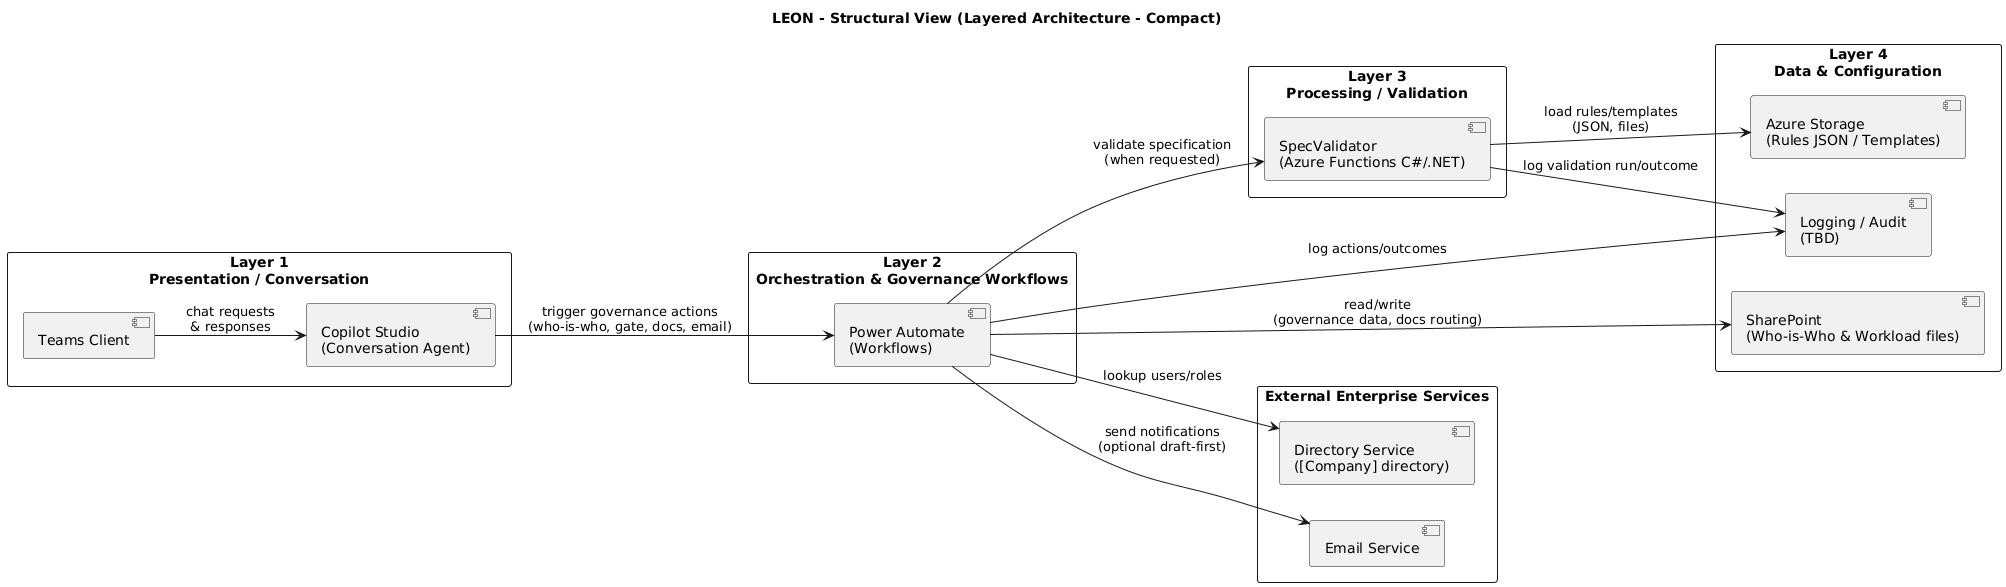
\includegraphics[width=0.9\textwidth]{images_pfe/structural view.png}
    \caption{Structural View: Architecture Diagram of LEON Components.}
    \label{fig:structural-view}
\end{figure}
\FloatBarrier
\vspace{-4pt}

The figure~\ref{fig:structural-view} presents the LEON architecture modeled according to the layers mentioned above. It highlights how the dialogue interface, orchestration capabilities, validation services and data sources interact with the activities related to governance.
% ═════════════════════════════════════════════════════════════════════════════
\section{\textcolor[HTML]{0066CC}{Dynamic View}}
\label{sec:design-dynamic-view}
% ═════════════════════════════════════════════════════════════════════════════

\subsection*{\textcolor[HTML]{003D99}{Primary Scenario: Specification Validation}}

Figure~\ref{fig:leon-sequence-en} shows the interaction sequence for specification validation in LEON.

\vspace{-8pt}
\begin{figure}[H]
    \centering
    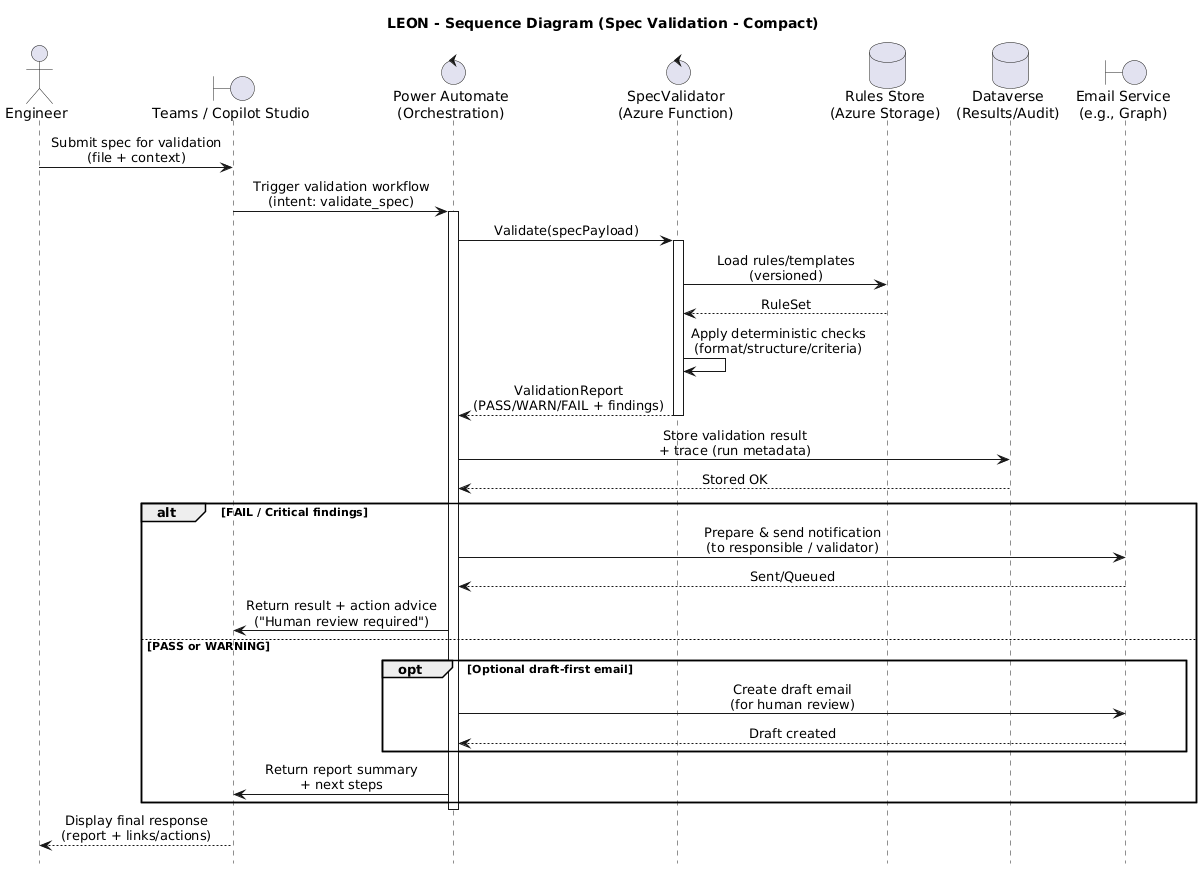
\includegraphics[width=0.9\textwidth]{images_pfe/sequence_diagram.png}
    \caption{UML Sequence Diagram: specification validation scenario showing interaction between Copilot Studio, Power Automate, SpecValidator, and Azure Storage.}
    \label{fig:leon-sequence-en}
\end{figure}
\FloatBarrier
\vspace{-4pt}

The sequence of events starts when the user inputs the specification in the conversational interface. The orchestration layer receives the entering specification request and starts the validation workflow.\\
The validation service receives the specification and uses a set of validation rules that is represented as a set of configuration information retrieved from the configuration layer. The result of validation is a formal validation report of the specification.\\
There are two execution flows according to the outcome. The critical problems would make the system execute other actions (e.g. notify interested people who should be responsible for that, request an expert review). The non-critical problem would make the system give back the overview of the validation with suggested action.\\
The result is then sent back to the user via the orchestration layer and is displayed through conversational interface.

% ═════════════════════════════════════════════════════════════════════════════
\section{\textcolor[HTML]{0066CC}{Data Model (Conceptual)}}
\label{sec:design-data-model}
% ═════════════════════════════════════════════════════════════════════════════

\subsection*{\textcolor[HTML]{003D99}{Key Conceptual Entities}}

Conceptual data model represents the core objects of the LEON governance process and the relations between these objects. It gives a high-level view on the structure of project data, responsibilities, validation and interaction.
\vspace{0.2cm}
\noindent\textcolor[HTML]{0066CC}{\textbf{Entities}}

\begin{description}
    \item[\texttt{Project}] A combination (in a folder) of components, deliverables and governance.
    
    \item[\texttt{Component}] Is the smallest logical and technical unit of a project. It can be tested, as one entity, and have a person or persons accountable.
    
    \item[\texttt{Actor/Responsible}] Human involved in governance, identified through the governance directory. A responsible may be a component owner or task owner.
    
    \item[\texttt{Gate}] Designates a stage in the project‘s life cycle (i.e. Gate 1, Gate 2, Gate 3) with specific validation needs and fields of competence
    
    \item[\texttt{Specification}] Technical document or deliverable of a component and a gate that can be validated.
    
    \item[\texttt{ValidationRule}] A preexisting rule providing the validation condition in accordance with specifications and context.
    
    \item[\texttt{Assignment}] assigning tasks to a person, considering his workload and scheduling constraints
    
    \item[\texttt{AuditLog}] The AuditLog object helps record what‘s being done within the system: what was doing it, who was doing it and when.
\end{description}

\subsection*{\textcolor[HTML]{003D99}{Primary Relationships}}

\begin{itemize}
    \item \textcolor[HTML]{003D99}{\textbf{Project} \texttt{1..N} \textbf{Component}} : a project contains multiple components.
    \item \textcolor[HTML]{003D99}{\textbf{Component} \texttt{1..N} \textbf{Responsible}} : a component may have multiple responsible parties (over time or by role).
    \item \textcolor[HTML]{003D99}{\textbf{Gate} \texttt{1..N} \textbf{ValidationRule}} : each gate is associated with a set of rules.
    \item \textcolor[HTML]{003D99}{\textbf{Specification} \texttt{N..1} \textbf{Gate}, \textbf{Component}} : each specification is linked to a Gate and Component.
    \item \textcolor[HTML]{003D99}{\textbf{Actor} \texttt{1..N} \textbf{Assignment}} : an actor may have multiple assignments.
    \item \textcolor[HTML]{003D99}{\textbf{AuditLog} \texttt{N..1} \textbf{Actor}} : each action is traced to the actor who performed it.
\end{itemize}

\subsection*{\textcolor[HTML]{003D99}{Conceptual Representation}}

\vspace{-8pt}
\begin{figure}[H]
    \centering
    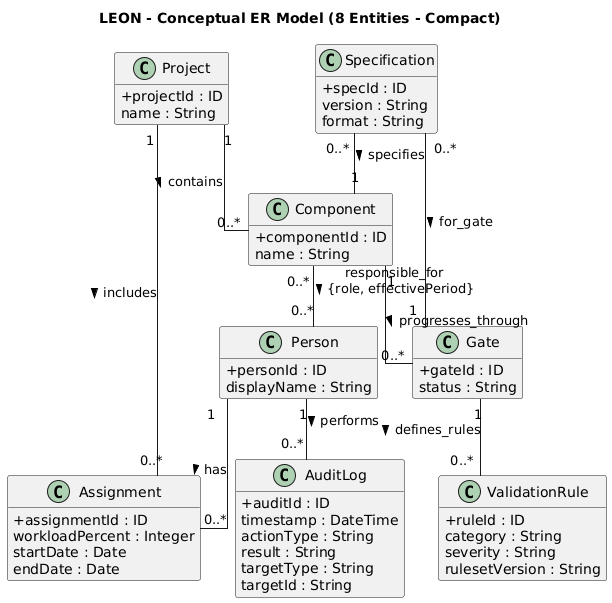
\includegraphics[width=0.9\textwidth]{images_pfe/conceptual ER.png}
    \caption{Conceptual Entity-Relationship Diagram of LEON.}
    \label{fig:conceptual-er}
\end{figure}
\FloatBarrier
\vspace{-4pt}
This diagram illustrates how the various components, the relation between entities and the governance data, the validation and system interaction are working together.


% ═════════════════════════════════════════════════════════════════════════════
\section{\textcolor[HTML]{0066CC}{V-Model: Design-to-Verification Traceability}}
\label{sec:design-vmodel}
% ═════════════════════════════════════════════════════════════════════════════
The V-Model (Verification \& Validation) establishes the complete traceability chain from design artifacts to verification evidence. Figure~\ref{fig:vmodel_leon} synthesizes:
\usetikzlibrary{positioning,arrows.meta,shapes.geometric}

\begin{figure}[H]
    \centering
    \begin{tikzpicture}[
        node distance=1.5cm and 2.5cm,
        every node/.style={align=center},
        artifact/.style={rectangle, draw, rounded corners, minimum width=3cm, minimum height=1cm, fill=blue!20},
        evidence/.style={rectangle, draw, rounded corners, minimum width=3cm, minimum height=1cm, fill=green!20},
        implementation/.style={rectangle, draw, minimum width=4cm, minimum height=1cm, fill=orange!20},
        trace/.style={dashed, -{Latex[length=3mm]}}
    ]

    % Left side (Definition/Design Artifacts)
    \node[artifact] (req) {Requirements \\ \& Use Cases \\ (Fig 5.1)};
    \node[artifact, below=of req] (arch) {Structural \\ Architecture \\ (Fig 5.3)};
    \node[artifact, below=of arch] (data) {Data Model \\ (Fig 5.5)};
    \node[artifact, below=of data] (dynamic) {Dynamic Scenario \\ (Fig 5.4)};

    % Bottom (Implementation)
    \node[implementation, below=of dynamic, yshift=-1cm] (impl) {Implementation \\ (Power Automate \\ + Azure Functions)};

    % Right side (Verification/Validation Evidence)
    \node[evidence, right=of req] (tests) {Scenario-based \\ Tests};
    \node[evidence, below=of tests] (validation) {Validation Report \\ Checks};
    \node[evidence, below=of validation] (access) {Access-Control \\ Checks};
    \node[evidence, below=of access] (audit) {Audit/Log \\ Verification};

    % Arrows (V-Model)
    \draw[-{Latex[length=3mm]}] (req) -- (arch);
    \draw[-{Latex[length=3mm]}] (arch) -- (data);
    \draw[-{Latex[length=3mm]}] (data) -- (dynamic);
    \draw[-{Latex[length=3mm]}] (dynamic) -- (impl);

    \draw[-{Latex[length=3mm]}] (impl) -- (audit);
    \draw[-{Latex[length=3mm]}] (audit) -- (access);
    \draw[-{Latex[length=3mm]}] (access) -- (validation);
    \draw[-{Latex[length=3mm]}] (validation) -- (tests);

    % Traceability Links
    \draw[trace] (req) -- (tests);
    \draw[trace] (arch) -- (validation);
    \draw[trace] (data) -- (access);
    \draw[trace] (dynamic) -- (audit);

    \end{tikzpicture}
    \caption{V-Model overview: traceability from requirements to verification artifacts in LEON.}
    \label{fig:vmodel_leon}
\end{figure}
\FloatBarrier
\vspace{-4pt}
\begin{itemize}
    \item \textcolor[HTML]{003D99}{\textbf{Left side (Definition phase)}} : Requirements \& Use Cases (Fig 5.1), Structural Architecture (Fig 5.3), Data Model (Fig 5.5), and Dynamic Scenario (Fig 5.4).
    \item \textcolor[HTML]{003D99}{\textbf{Bottom (Implementation)}} : Power Automate workflows and SpecValidator service realization.
    \item \textcolor[HTML]{003D99}{\textbf{Right side (Verification phase)}} : Scenario-based tests, validation report checks, access-control verification, and audit/log traceability.
    \item \textcolor[HTML]{003D99}{\textbf{Dashed traceability links}} : connect each left-side artifact to its corresponding verification evidence on the right.
\end{itemize}




% ═════════════════════════════════════════════════════════════════════════════
% Chapter 10: Implementation and Realization of LEON
% ═════════════════════════════════════════════════════════════════════════════

\chapter{Implementation and Realization of LEON}
\label{chap:implementation}

% ═════════════════════════════════════════════════════════════════════════════
\section{\textcolor[HTML]{0066CC}{Implementation Scope and Delivered Features}}
\label{sec:impl-scope}
% ═════════════════════════════════════════════════════════════════════════════

This chapter details the realization of LEON following the design architecture presented in Chapter~\ref{chap:design}. The implementation phase focused on delivering two primary blocks---Governance services and SpecValidator---integrated through Copilot Studio's conversational orchestration layer, including advanced topic-based routing for dynamic dialogue management.

\subsection{\textcolor[HTML]{003D99}{Mapping to Strategic Objectives}}

\begin{table}[H]
    \centering
    \small
    \caption{Mapping of implemented features to strategic objectives.}
    \label{tab:impl-so-mapping}
    \begin{tabularx}{\textwidth}{|l|l|X|}
        \hline
        \textbf{SO} & \textbf{Feature} & \textbf{Implementation Component} \\
        \hline
        SO1 & Conversational access to governance data & Copilot Studio agent, Topics, Power Automate flows \\
        \hline
        SO2 & Who-is-Who responsible lookup & Copilot Studio knowledge base, PA flow connector \\
        \hline
        SO3 & Gate status and artifact tracking & Copilot Studio knowledge base, SharePoint integration \\
        \hline
        SO4 & Deterministic spec validation & Azure Functions, C\#, detailed report \\
        \hline
        SO5 & Complete audit and compliance traceability & Copilot Studio audit logs, Power Automate logging \\
        \hline
    \end{tabularx}
\end{table}

\subsection{\textcolor[HTML]{003D99}{Delivered Artifacts}}

The creation of the set of functional artefacts and technical artefacts generated during LEON implementation, was structured on the system architecture. Each artefact corresponds to one of the solution‘s layers and reflects the implementation of the elements created.

\textcolor[HTML]{0066CC}{\textbf{Layer 1: Conversational Interface}}

The conversational interface is executed by a Copilot Studio agent. The agent allows natural language conversation and acts as the principal interface to the system.

It has a list of conversational topics (about six core ones) that map to the governing services:  Who-is-Who, gate monitor, responsibility change, upload document,  handle task and notify.  They drive the dialogue logic and connect user intents to the desired services.

\vspace{0.4cm}

\textcolor[HTML]{0066CC}{\textbf{Layer 2: Orchestration and Business Logic}}

The system activities are then handled by the Power Automate flows. The triggers are the Copilot Studio topics that enforce the business logic around the governance activities.

The flows perform the following primary functionalities; requesting for responsibility data, Gate status data, updating assignments, loading data and notifying the stakeholders and calling external enterprise‘s services.

\vspace{0.4cm}

\textcolor[HTML]{0066CC}{\textbf{Layer 3: Data Management and Knowledge Base}}

The proposed system is founded on a layered knowledge base composed of the governance knowledge base and the resource configuration, including Who-is-Who, gaterelated information, and workload information.

These data elements is stored in enterprise repositories and are dynamically read by the orchestration layer in order to fulfill the user requests.

\vspace{0.4cm}

\textcolor[HTML]{0066CC}{\textbf{Layer 4: Validation and Specification Assessment}}

For the validation process we use a service called SpecValidator which carries out a determinist evaluation of the technical specifications.

This component receives defined validation rules and runs them on input documents  and generates a formal report of validation outcomes and suggestions.  Rule repository is created for validation logic,  and consistent assessment is sustained.

\vspace{0.4cm}

\textcolor[HTML]{0066CC}{\textbf{Layer 5: Logging and Audit Traceability}}

Log management systems are built to log system trace and user action requirements to meet auditing requirements and compliance issues.

These logs might be tracking specific events like getting the data, updating, the outcome messages of validation, and notification etc. in order to facilitate the tracking.

\vspace{0.4cm}

In conclusion,  this collection of artifacts makes up the LEON system with conversational dialogue, workflow execution and management, validation execution and data processing within a single system to perform the governance operations.

% ═════════════════════════════════════════════════════════════════════════════
\section{\textcolor[HTML]{0066CC}{Implementation Environment}}
\label{sec:impl-environment}
% ═════════════════════════════════════════════════════════════════════════════

\subsection{\textcolor[HTML]{003D99}{Technology Stack}}

LEON is presented in a cloud enterprise environment, merging the components of Conversation AI, workflow orchestration, validation engine, and data services. The components selected adhere to the layer architecture presented in Chapter 4 and present a modular and extensible platform.

\vspace{0.3cm}
\noindent\textcolor[HTML]{0066CC}{\textbf{1. Conversational Layer}}

User interaction is managed through Microsoft CoPilot Studio, which provides a conversational interface (users can speak with the system). It maps the user requests to the services by understanding the user intent, managing context and pushing the request to the needed service via some defined topics.

\begin{figure}[H]
  \centering
  
\includegraphics[width=0.48\textwidth]{images_pfe/copilot studio.jpg}
  \caption{Microsoft CoPilot Studio interface used for conversational interactions.}
  \label{fig:copilot_studio}
\end{figure}

\vspace{0.3cm}
\noindent\textcolor[HTML]{0066CC}{\textbf{2. Orchestration Layer}}

Microsoft Power Automate represents the orchestration of the system functions that the conversational interface interacts with, and also where the business logic of the governance is implemented for actions such as looking up who is responsible, what the status of a gate is, processing documents, processing notifications, the layer calls on other external enterprise systems to do those actions.

\begin{figure}[H]
  \centering
  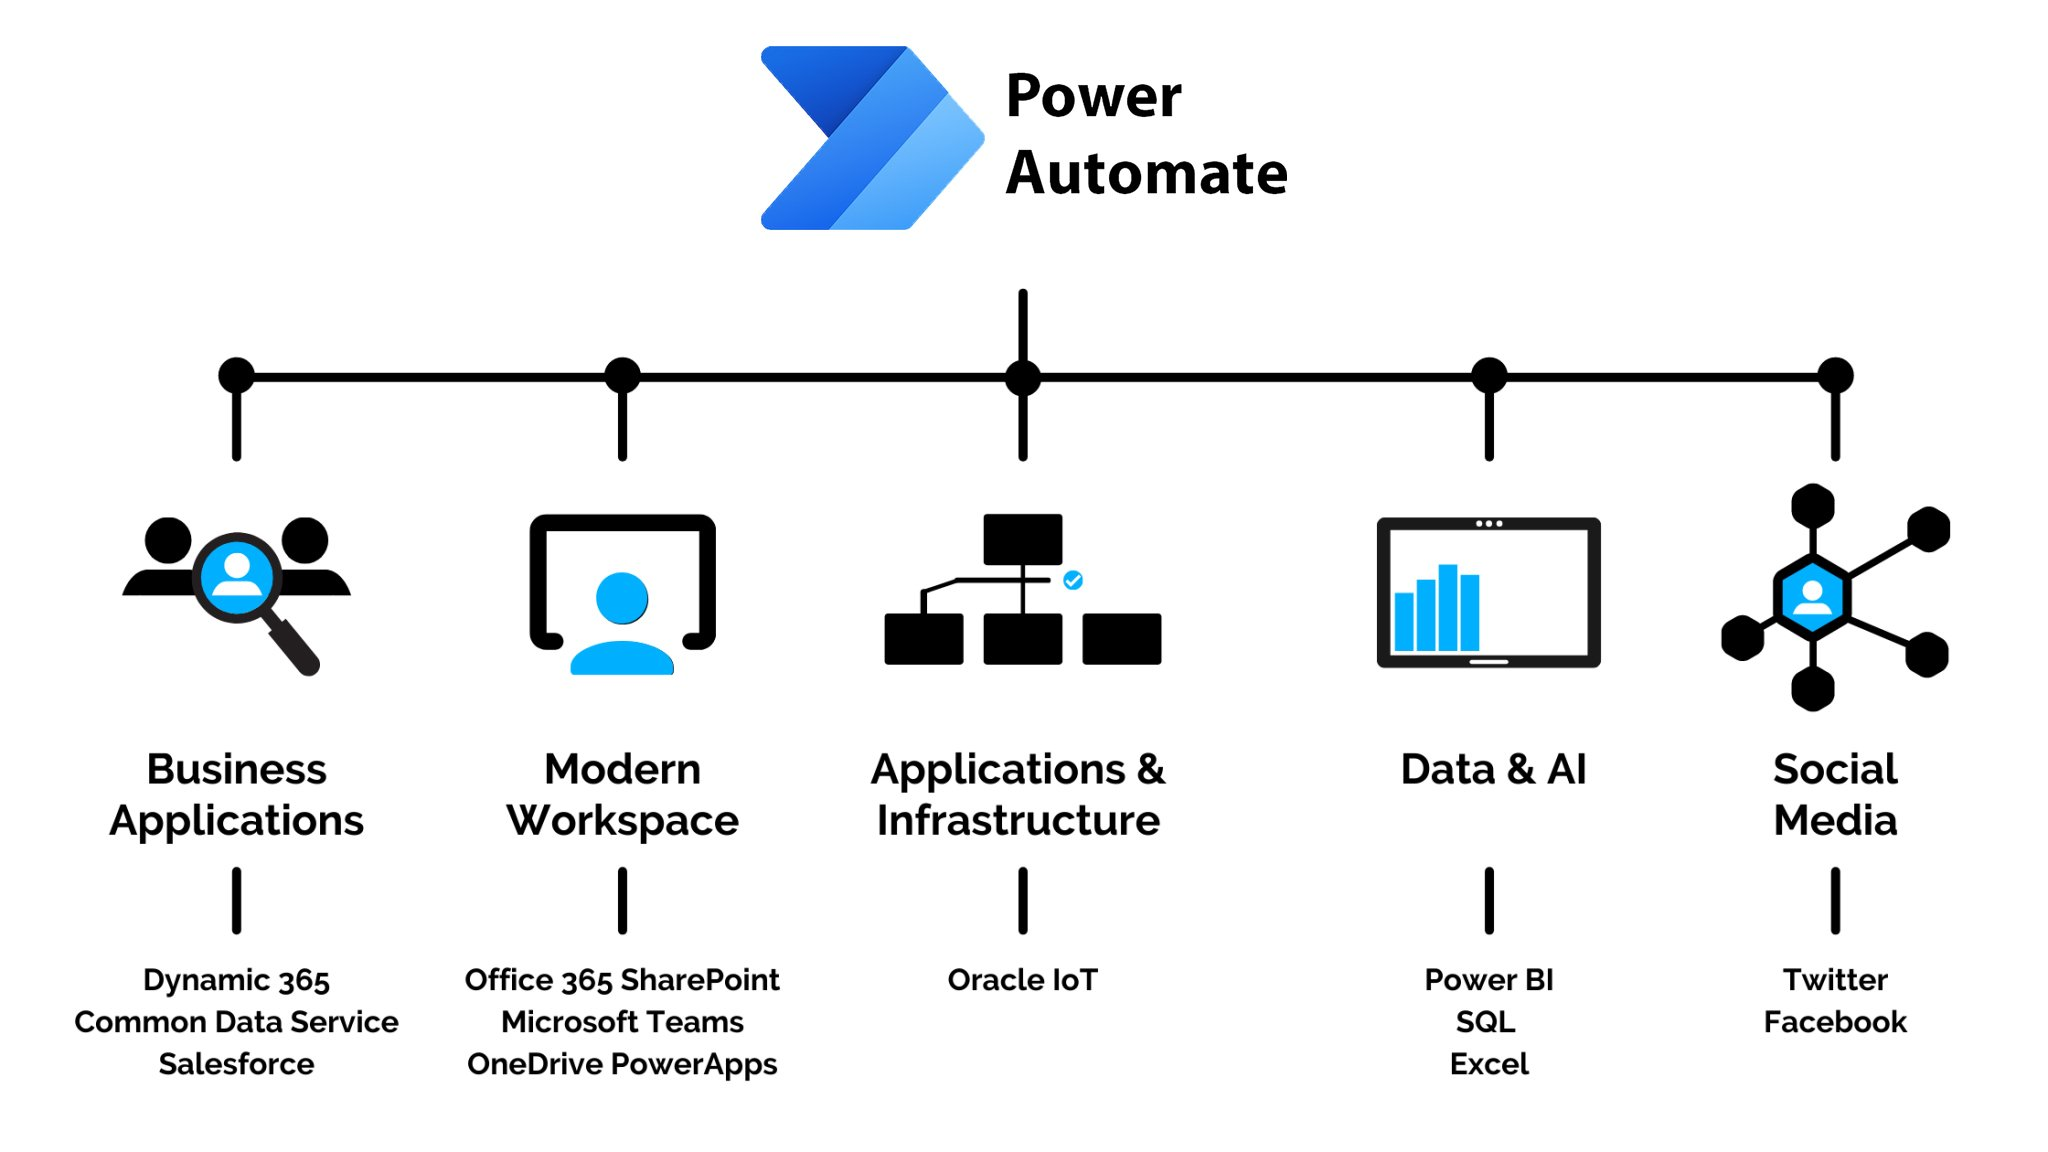
\includegraphics[width=0.48\textwidth]{images_pfe/power automate.jpg}
  \caption{Microsoft Power Automate interface used for orchestration interactions.}
  \label{fig:power_automate}
\end{figure}

\vspace{0.3cm}
\noindent\textcolor[HTML]{0066CC}{\textbf{3. Validation Layer}}

The specification validation runs by a defined service that uses Azure Functions, it takes the technical specification as input and executes the configured rules to return a validated report. It does not affect the conversation flow, which makes it deterministic and reproducible.

\begin{figure}[H]
  \centering
  
\includegraphics[width=0.48\textwidth]{images_pfe/azure function.png}
  \caption{Azure Functions interface used for validation interactions.}
  \label{fig:azure_functions}
\end{figure}

\vspace{0.3cm}
\noindent\textcolor[HTML]{0066CC}{\textbf{4. Data Management Layer}}

At this level the system utilizes several different data stores, which support governance and validation activities such as the conversational interface that uses structured data store, the enterprise document store (real time governance data and deliverables) and the configuration store (validation rules and templates).

\begin{figure}[H]
  \centering
  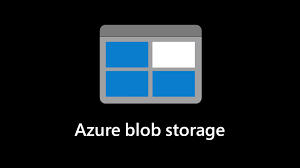
\includegraphics[width=0.48\textwidth]{images_pfe/Azure Storage.png}
  \caption{Azure Storage interface used for data management interactions.}
  \label{fig:azure_storage}
\end{figure}

\vspace{0.2cm}

To conclude, this combination of technologies enables LEON to orchestrate dialogues and automate processes, while allowing data to be accessed and validated through a single system. It complements the system specification and offers a flexible way to manage governance processes in an enterprise environment.

\subsection{\textcolor[HTML]{003D99}{Deployment Architecture (Multi-Environment)}}

LEON deployment strategy is centered around multi-environment where it is built, tested and released to production in a controlled and monitored way which is compatible with the Stellantis enterprise system. This process enables safe evolution of the system without compromising its reliability and controllability during the implementation.

Three main environments are used:\\

\vspace{0.2cm}
\noindent\textcolor[HTML]{0066CC}{\textbf{A. Development Environment (Dev)}}

Development Environment is an environment that allows for the fast prototyping and incremental development of new features. Within this environment the developers are able to design and test conversation flows, workflows, and validation logic without relying on production data. In essence, this is a sandbox in which to test and debug quickly.\\

\vspace{0.2cm}
\noindent\textcolor[HTML]{0066CC}{\textbf{B. Test Environment (Test)}}

The test environment is the staging environment used to run the implemented functions and ensure they work, prior to reaching the production environment. It is used in the process of testing scenarios and performing UAT (User Acceptance Testing).\\

\vspace{0.2cm}
\noindent\textcolor[HTML]{0066CC}{\textbf{C. Production Environment (Prod)}}

This is where LEON is installed and connected to Stellantis end users. This is the environment which can support verified configuration and fixed workflow. The environment where end users can use LEON governance services and validation functions.

\vspace{0.3cm}
\noindent\textcolor[HTML]{003D99}{\textbf{Environment Promotion Strategy}}

Promoted to environments carefully, configurations and work flows will be transported step by step to Development, to Test, then to Production. With this, we can allocate enough time to validation and testing, and do not have to work with untested components until the final users.

\vspace{0.3cm}

This multi environment architecture manages the evolution of system with safety as it segregates system into isolated environment on top of a shared data architecture. This approach will improve the deployment, maintain the system stability and allow a stepwise evolve of LEON without compromise on enterprise integrity.

% ═════════════════════════════════════════════════════════════════════════════
\section{\textcolor[HTML]{0066CC}{Governance Block Implementation}}
\label{sec:impl-governance}
% ═════════════════════════════════════════════════════════════════════════════

Users interact with LEON's Governance block to manage project components, roles, and responsibilities—all through natural conversation. Rather than switching between Excel spreadsheets, project management tools, and email, engineers simply ask LEON questions: ``Who is responsible for the brake system in J4U?'' or ``Update the DRE for the dashboard to John Smith.''

The Governance block connects three core components: (1) Copilot Studio manages the conversation and understands user intent, (2) Power Automate orchestrates the business logic and data updates, and (3) Excel spreadsheets on SharePoint store the governance data. This architecture works because it integrates with tools that Stellantis teams already use—there's no new system to learn.

This section details how five governance services function: how topics route conversations to the right handler, how LEON looks up component responsibilities, how it tracks project gates, how it updates assignments when engineers change roles, and how it manages document uploads to gate milestones.

\vspace{0.3cm}
\noindent\fbox{%
    \parbox{0.95\textwidth}{%
        \textcolor[HTML]{0066CC}{\textbf{Governance Services at a Glance:}} Users ask questions about project components, LEON queries Excel governance data through Power Automate, and responds conversationally. Updates are logged for compliance, and affected teams receive notifications automatically.
    }%
}
\vspace{0.3cm}

\subsection{\textcolor[HTML]{003D99}{Copilot Studio Topics and Conversation Design}}
\label{sec:impl-topics}

\subsubsection{Topic Architecture}

Topics are the core orchestration mechanism in Copilot Studio. Each governance service is mapped to one or more topics:

\begin{center}
\begin{tabularx}{0.95\textwidth}{|l|X|X|}
    \hline
    \textbf{Topic} & \textbf{User Query} & \textbf{Associated Functions} \\
    \hline
    \textbf{Who-is-Who Search} & ``Who is responsible for component [Component]?'' & Lookup flow trigger \\
    \hline
    \textbf{Gate Status} & ``What is the current gate for [Component]?'' & Gate metadata retrieval \\
    \hline
    \textbf{Update Responsible} & ``Update responsible for [Component] to [New Name].'' & Update flow with RBAC validation \\
    \hline
    \textbf{Upload Deliverable} & ``Upload my specification for gate [Gate].'' & File attachment and SharePoint routing \\
    \hline
    \textbf{Workload Management} & ``Show me my workload.'' & Assignment retrieval and updates \\
    \hline
    \textbf{Send Notification} & ``Send a reminder to [actor].'' & Email trigger via Power Automate \\
    \hline
    \textbf{Escalate} & Unresolved queries & Human support team escalation \\
    \hline
\end{tabularx}
\end{center}

\subsubsection{Knowledge Base Integration}

The Copilot Studio knowledge base organizes governance data into structured repositories:

\begin{itemize}
    \item[\quad\textbullet] \textcolor[HTML]{003D99}{\textbf{Who-is-Who dataset}} : Excel file with Project, Component, Responsible Name, Responsible Email, Role, Active columns.
    \item[\quad\textbullet] \textcolor[HTML]{003D99}{\textbf{Gate metadata}} : Project, Component, Current Gate, Gate Entry Date, Expected Exit Date, Gate Owner.
    \item[\quad\textbullet] \textcolor[HTML]{003D99}{\textbf{Validation guidelines}} : Acceptance criteria documentation per gate level.
    \item[\quad\textbullet] \textcolor[HTML]{003D99}{\textbf{SharePoint data connectors}} : Real-time links to governance lists and tables for live queries.
\end{itemize}

\noindent Entity extraction via NLU processes user utterances and queries these knowledge sources to provide contextual answers.

\subsection{\textcolor[HTML]{003D99}{Implementation: Who-is-Who Responsible Lookup}}
\label{sec:impl-whoiswho}

\subsubsection{Objective and Scope}

The Who-is-Who responsible lookup service can be used by the user to discover the person accountable for a component within a project using query (via excel) into the governance data source. This can be triggered conversationaly through Copilot studio by using Power Automate flows and will provide an accountable person identifier or an error code (managed through conversational invocation) as output.
\subsubsection{Where the Data Lives}

LEON counts on Stellantis governance teams which used to be responsible for mapping component responsibility in Excel. Therefore, instead of building up a database, LEON is just linked to the excel on SharePoint. This implies that:
\begin{itemize}
    \item Same modification done by the Governance engineers as it has been before
    \item LEON auto-reads changes automatically with no workflow.
    \item Permissions are inherited. If one user is allowed to change the spreadsheet, then this user can start an update through LEON.
    \item Teams will not play around with new tools. It‘s just that the information becomes readily available.
\end{itemize}

\begin{figure}[H]
    \centering
    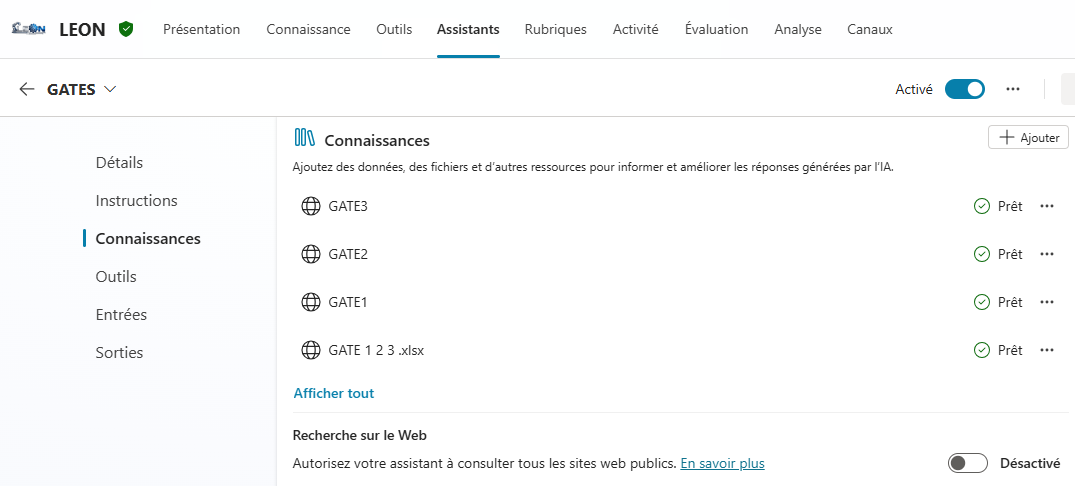
\includegraphics[width=0.5\textwidth]{images_pfe/knowledge gate.png}
    \caption{Who-is-Who Excel structure: Each project gets a sheet (J4U, SP1-P1H, etc.), components are rows, roles are columns.}
    \label{fig:w1-dataset-structure}
\end{figure}

\noindent\textbf{File Organization:}

\begin{itemize}
    \item[\quad\textbullet] \textbf{One Excel file}: The workbook is the single source for governance data.
    \item[\quad\textbullet] \textbf{Multiple sheets}: Each sheet has the name of the corresponding project (e.g. “J4U”, “SP1-P1H”, “X2Y”). New projects should be associated with a new sheet.
    \item[\quad\textbullet] \textbf{Sheet structure}: Each sheet employs identical tabular layout for consistency:
    \begin{itemize}[leftmargin=0.5cm]
        \item \textcolor[HTML]{003D99}{\textbf{First column}} :  Is a “Component” header, component ids that are unique within the project.
        \item \textcolor[HTML]{003D99}{\textbf{Subsequent columns}} :  Organization role headers (i.e. “DRE”, “DL”, “Pilot”, “Global CTE”) and person names in the cells.
        \item \textcolor[HTML]{003D99}{\textbf{Header row}} : The role name should be in the first row of each sheet and the role may differ among each:
    \end{itemize}
    \item[\quad\textbullet] \textbf{Cell values}: In the intersection of component row and role column name of responsible person should be displayed if only one. If there are more than one responsible persons, it has to be separated using either “/” or “,” based on how it is written in the table.
    \item[\quad\textbullet] \textbf{Empty cells}: Show that there is no accountable person for the specific combination of component-role.
    \item[\quad\textbullet] \textbf{Dynamic identification}:  Order of columns and role names can be identified dynamically per sheet and is not fixed, therefore giving the flexibility.
\end{itemize}

\noindent The excel multiple tab structure is extremely flexible, new projects are created by adding new sheets to the spreadsheet and new roles can be created by adding more columns of data to the table.



\subsubsection{How the Lookup Works: A Real Example}

An engineer may ask (e.g. ” DRE of brake system for the J4U project ? ”). The answer LEON gives :

\begin{enumerate}
\item \textbf{Understands intent:} Copilot NLU finds three attributes that are the J4U project, the brake system component and the role of DRE.
\item \textbf{Finds the project sheet:} LEON checks if J4U matches any sheet name in the Excel file
\item \textbf{Locates the component row:} In the Component column, LEON seeks out “brake system” (or similar, if not exactly).
\begin{figure}[H]
    \centering
    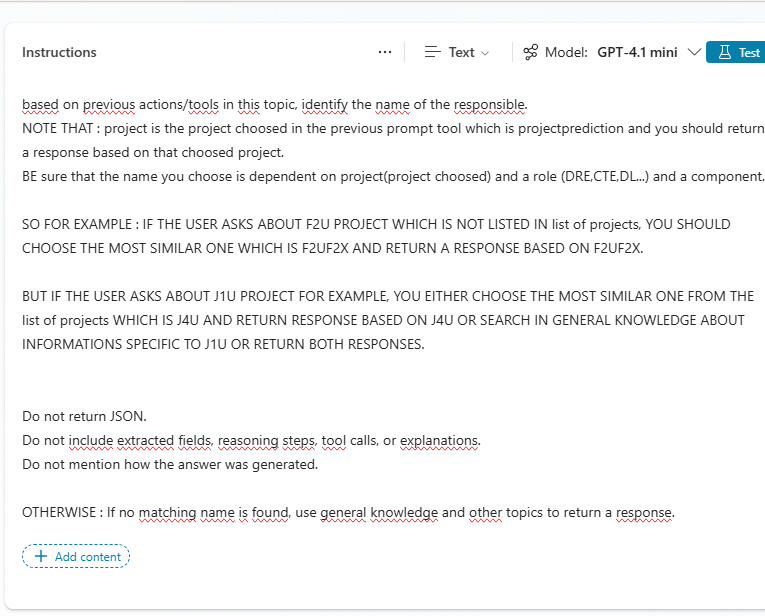
\includegraphics[width=0.85\textwidth]{images_pfe/name search.png}
    \caption{Component search workflow: Locating component row in Excel.}
    \label{fig:w4-lookup}
\end{figure}
\item \textbf{Finds the role column:} Looks across the first row for the DRE column header
\item \textbf{Returns the answer:} LEON reads the cell at the intersection and finds the responsible engineer's name
\end{enumerate}


\textbf{Why this design matters:} Engineers doesn‘t need to provide the exact string in Excel because there is a phase of normalization (case insensitive, trimming leading and trailing spaces) that handles all inputs of the users. The tolerance is good for user as there is less confusion and less question.

\subsubsection{Handling Project Name Ambiguity}

Not all of the users and enginners remembers the exact project codes or names. While testing the pilot program we had discover that:

\begin{itemize}
\item The variation of cases (”J4U” vs “j4u”, etc)
\item Some institutions (or engineers) write abbreviations (``J4'' instead of ``J4U'')
\item Many also use codenames or nicknames for projects rather than their official designation.
\end{itemize}

To handle this, we implemented a two-step matching process:

\textbf{Step 1: Exact Match (Case Insensitive)}  
LEON converts the user input to lower case and compares it with the names of the excel sheets. If there is sheet called J4U and the user enters either j4u or J4u, there is a matching case.

\textbf{Step 2: Similarity Fallback}  
Similarity fallback if there are no exact matches, we are looking for partial matches. The engineer who gives “the automotive project four” to the system, will not be able to find the “J4U” name. We don‘t want to filter the engineer but assist him. Copilot, using NLU, will search and provide him the closest matching name and will suggest it by asking him: “did you mean the J4U project ?” to prevent any potential escalation.

\subsubsection{Finding the Right Cell}

Upon approval of the project sheet, LEON attempts to find the component and the role in it. This step might seem straightforward at first, but has some practical drawbacks:


\begin{itemize}
\item \textbf{Component naming varies:} In one project, the engineer uses ‘extermirrors’, the other one use ‘ext.mirrors’ or just ‘MirrorSystem’. We accept missing spaces and ignore case while matching, and calculate the similarity score
\item \textbf{Role columns differ by project:}  In J4U, there are “DRE”, “Pilot”, and “CTE”, whereas in SP1-P1H there are “DL”, “Global CTE”, and “Quality Lead”. The headers will be dynamically read in, rather than hard coded.
\item \textbf{Multiple responsibilities:} There are situations where one cell is responsible for more than one individual; such as “Jane Smith / John Doe”. LEON presents back the two individuals to the user.
\end{itemize}

\subsubsection{Error Handling and Fallback}

\noindent The service produces the following error conditions:

\vspace{0.15cm}

\begin{tabularx}{0.95\textwidth}{|l|X|}
    \hline
    \textbf{Error} & \textbf{What Went Wrong} \\
    \hline
    \texttt{PROJECT NOT FOUND} & User said a project name that doesn't exist. Copilot suggests available projects. \\
    \hline
    \texttt{COMPONENT NOT FOUND} & Component not in the sheet we return this rather than guessing. \\
    \hline
    \texttt{ROLE NOT FOUND} & Requested role (e.g., ``CEO'') doesn't exist in that project's columns. \\
    \hline
    \texttt{RESPONSIBLE NOT ASSIGNED} & Cell is empty ,no one assigned to that component role yet. \\
    \hline
    \texttt{DATASET UNAVAILABLE} & SharePoint is down or network issue. User retries later. \\
    \hline
    \texttt{UNAUTHORIZED} & User lacks permission to read that project. Security enforced at Excel level. \\
    \hline
\end{tabularx}





\subsubsection{Output Format}

Who-is-Who lookup is showing one of the outcomes only, it depends upon execution.

\begin{itemize}
    \item[\quad\textbullet] \textbf{Success}: If it is a success, server sends to client cell contents (a cell, one or many names) exactly like it is saved in the cell in excel (without any pre-treatment).
    \item[\quad\textbullet] \textbf{Error}: When the lookup fails the function returns an error code such as for instance \texttt{PROJECT NOT FOUND} which will be mapped by Copilot Studio into a conversational response.
    \begin{figure}[H]
    \centering
    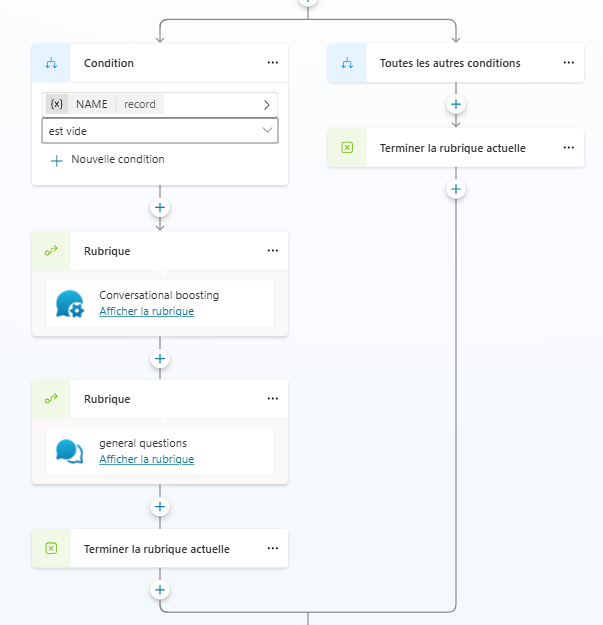
\includegraphics[width=0.9\textwidth]{images_pfe/condition who.png}
    \caption{Error condition handling workflow: Decision tree for error scenarios in Who-is-Who lookup.}
    \label{fig:w5-error-condition}
\end{figure}
\end{itemize}



\subsection{\textcolor[HTML]{003D99}{Implementation: Gate Status Retrieval}}
\label{sec:impl-gatestatus}

\subsubsection{Why Gate Status Matters}

The development process of an automotive product involves gates : Gate 1 for concept, Gate 2 for detail design, Gate 3 for pre-production. The engineers will want to know: ” Has the brake system reached Gate 2 ? ”. This then determines the relevant design reviews that are needed.

While Who is Who is nothing more than a lookup on an excel table, gate status is kept in documents. When a component passes through a gate the spec is stored in a SharePoint folder, namely, ’/LEON-Governance/J4U/Gate-2/Brake-System/’. Then Gate Status is determined by looking through the folders where a particular document resides.

\textbf{Why this approach?} The gates are a governance mark used by Stellantis. we are reading files, so we would not be inventing a new system to be updated if metadata were separated from the other parts of information. The guess is that gate 3 is skipped or served much more rapidly if gate 3 is present in the catalog but not gate 2.

\subsubsection{Data Source}

The status of a gate is inferred via a knowledge structure in the documents with three gate levels:

\begin{figure}[H]
    \centering
    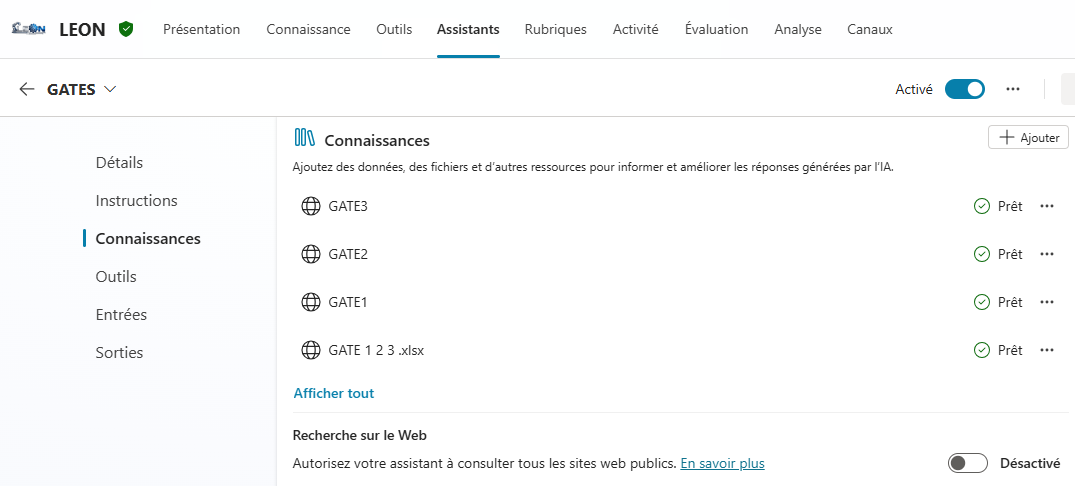
\includegraphics[width=0.85\textwidth]{images_pfe/knowledge gate.png}
    \caption{Knowledge base organization: Gate 1, Gate 2, and Gate 3 document repositories.}
    \label{fig:gate-knowledge-structure}
\end{figure}

\begin{itemize}
    \item[\quad\textbullet] \textbf{GATE1}: Knowledge source/folder contains documents associated with Gate 1 deliverables.
    \item[\quad\textbullet] \textbf{GATE2}: Knowledge source/folder contains documents associated with Gate 2 deliverables.
    \item[\quad\textbullet] \textbf{GATE3}: Knowledge source/folder contains documents associated with Gate 3 deliverables.
\end{itemize}

\subsubsection{How Documents Signal Gate Progress}

Project documentation on Stellantis is stored on SharePoint and organized by project, then by gate. Upon the brake system reaching Gate 2, the specification is placed on ”/LEONGovernance/J4U/GATE2/Brake-System/”. LEON is responsible for identifying which gate folders the component specification shall be forwarded:
\begin{itemize}
    \item[\quad\textbullet] \textbf{GATE1}: Concept documents for components that were approved for design phase
    \item[\quad\textbullet] \textbf{GATE2}: Design documents for components that passed detailed design review
    \item[\quad\textbullet] \textbf{GATE3}: Pre-production documents for components that are ready for manufacturing
\end{itemize}

When there are documents relating to the GATE2 Brake System, but not for the GATE3 component, the reasoning applied is that the component is in GATE2. When the GATE1 & GATE3 exist, but GATE2 is empty, the reasoning is that the component skipped GATE2, (or has an accelerated review process).
\vspace{0.2cm}

\noindent\textbf{Understanding the Query:}

For the query: “What gate is the suspension system at in J4U?”, Copilot NLU would return: project = J4U, component = suspension system. Both would be normalized to, say: “j4u” normalized to “J4U”, “suspension system”, and “suspension subsystem”. Using case insensitive prefix matching and substring search the parser can map all those strings appropriately.
\subsubsection{How LEON Finds the Gate}

The search process is straightforward:

\begin{enumerate}
    \item \textbf{Check Gate 3 first} (most advanced): Is there a file in ‘LEON Governance/J4U/GATE3/Suspension-System/’? Yes, your component is in Gate 3.
    \item \textbf{If not, check Gate 2}: If not, then try Gate 2: Is ”/“LEON-Governance/J4U/GATE2/Suspension-System/” with documents? if yes Gate 2.
    \item \textbf{If not, check Gate 1}: Otherwise: check Gate 1, find whether ’/LEON-Governance/J4U/GATE1/Suspension-System/’ exists in documents or not. If it exists, Gate 1.
    \item \textbf{If nothing found}: Component not at a recorded gate. LEON tells user: ” The suspension system has not yet been formally recorded at a gate”.
\end{enumerate}

\begin{figure}[H]
    \centering
    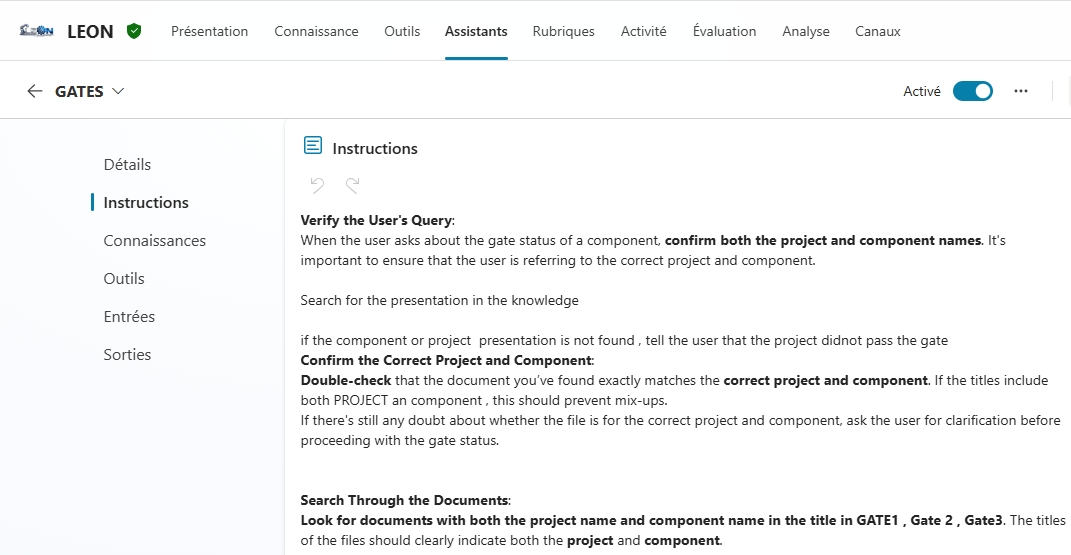
\includegraphics[width=0.45\textwidth]{images_pfe/gate1.png}
    \hfill
    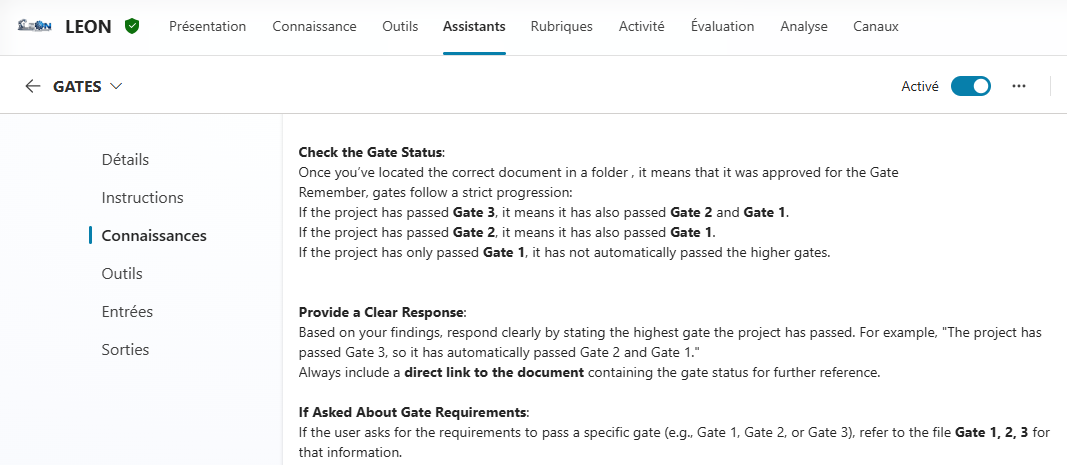
\includegraphics[width=0.45\textwidth]{images_pfe/gate2.png}
    \caption{Gate detection workflow: (left) document search across gate repositories; (right) highest gate level identification.}
    \label{fig:gate-detection-workflow}
\end{figure}

This document outlines the detection method that will be based on asserting that gate status is representative of the knowledge bases uploaded objects and stored objects that have not activated some other attribute to denote metadata.

\subsubsection{Error Handling and Fallback}

The service produces the following error or incomplete-result conditions:

\vspace{0.15cm}

\begin{tabularx}{0.95\textwidth}{|l|X|}
    \hline
    \textbf{What Happens} & \textbf{What LEON Does} \\
    \hline
    \texttt{PROJECT NOT FOUND} & Project doesn't exist in documents. LEON suggests alternatives: ``Did you mean J4U or SP1-P1H?'' \\
    \hline
    \texttt{COMPONENT NOT FOUND} & Component name doesn't match anything in that project. LEON asks: ``Which component? I can search available ones.'' \\
    \hline
    \texttt{NO GATE REACHED} & Valid project and component, but no gate documents found yet. LEON responds: ``The brake system hasn't reached a gate yet.'' \\
    \hline
    \texttt{KNOWLEDGE BASE UNAVAILABLE} & SharePoint is down or network issues prevent document search. LEON says: ``I can't access the gate documents right now. Try again in a moment.'' \\
    \hline
    \texttt{AMBIGUOUS MATCH} & Multiple documents with similar names (e.g., brake-system-v1, brake-system-final). LEON asks user to clarify which one. \\
    \hline
\end{tabularx}

\vspace{0.2cm}

\noindent For any error condition, Copilot Studio routes to fallback topic (Escalate) or requests user clarification.

\subsubsection{Output Format}

The Gate Status service returns a conversational response indicating:

\begin{itemize}
    \item[\quad\textbullet] \textbf{Success}: Identified at gate level (GATE1, GATE2 or GATE3) in a natural language. Example: Seat Actuator component in the project of XEV has reached GATE2 based on documents in the knowledge base.
    \item[\quad\textbullet] \textbf{Incomplete}: Clarification that we have not reached a documented gate. Example: Seat Actuator component in the project of XEV has not yet reached a documented gate.
    \item[\quad\textbullet] \textbf{Error}: error message and suggestions for next steps (refined search, confirmation, escalation)
\end{itemize}

\paragraph{Extension: Gate Document Upload (In Development)}

A further functionality that is under development and that allows the user to upload files to a particular gate:

\begin{enumerate}
    \item \textcolor[HTML]{003D99}{\textbf{User input}} : Upload deliverable for this excat component in this project inside the gate1. (with file attachment)
    \item \textcolor[HTML]{003D99}{\textbf{Copilot processing}} : extracts project, component, gate level, and file.
    \item \textcolor[HTML]{003D99}{\textbf{Validation}} : for each one of the three parameters (project, component, gate) check that it is well specified and that it exists.
    \item \textcolor[HTML]{003D99}{\textbf{Storage}} : The document should be uploaded in the correct gate repository (more specific folder GATE1, GATE2, GATE3 under the Knowledge Source). A file will be registered with its metadata such as Uploader, Creation date, Project, Component and Gate.
    \item \textcolor[HTML]{003D99}{\textbf{Logging}} : log the upload event to audit trail (timestamp, user identity, file, gate, status).
    \item \textcolor[HTML]{003D99}{\textbf{Response}} : confirm successful upload with file reference and gate location.
\end{enumerate}

\textbf{Note:} This feature (upload) is not yet implemented but it is scheduled for next release so that the components are sent to gates by the user who manage files by the LEON.

\subsection{\textcolor[HTML]{003D99}{Implementation: Responsible Assignment Update}}
\label{sec:impl-responsible-update}

\subsubsection{When Responsibilities Change}

Product development teams evolve. When a responsible moves to a new role, a new responsible takes over as his role for a specific componenet. When a design review is assigned to a new engineer, that person’s name needs to appear in the governance record.

Instead of Governance teams updating themselves in excel: find sheet, row, and column, added new name, saved file, e-mailed. With LEON: Updated the DRE for dashboard component in J4U to Sarah Chen and updated right away. It also logs who and when made the update, and what the change actually was, useful for auditable history of development.

\subsubsection{Where Updates Happen}

Updates are made to the same Excel file where Who-is-Who queries to. File has one sheet per project (J4U, SP1-P1H) where each component is a row and in each role we have a column. Updating DRE for the brake system to Sarah Chen, it means we update one cell in the J4U excel file, in the row brake system and in the column DRE. LEON is doing it via Power Automate excel connector, which has complete write permissions to the shared governance file.

\textbf{Why this matters:} All this information is readily available from the governance groups. We are not building yet another place to try and keep in sync. Updates to LEON are visible immediately when you open the Excel, and if a governance engineer makes a change directly into the Excel it will show up in the following query.

\subsubsection{What Information LEON Needs}

To make an update for the name of a responsible in a project, LEON needs four pieces of information:

\begin{itemize}
    \item[\quad\textbullet] \textbf{Project}: Which project? (J4U, SP1-P1H, etc.), the user should choose the project sheet to update.
    \item[\quad\textbullet] \textbf{Component}: Which component? (Brake System, Dashboard, etc.), the user should choose the component to update.
    \item[\quad\textbullet] \textbf{Role}: Which role? (DRE, Pilot, CTE, etc.), the user should choose the role to update.
    \item[\quad\textbullet] \textbf{New Name}: Who is responsible now? The user should provide the new name of the responsible.
\end{itemize}

In case the article is missing Copilot asks the user to provide the missing information. Similarly to the Who-is-Who service LEON is not sensitive to format.

\subsubsection{How the Update Happens}

This is how LEON processes the request of an engineer asking for ‘Update the DRE for External mirrors in J4U to John Doe’:
\begingroup
\setlength{\intextsep}{6pt}
\setlength{\textfloatsep}{6pt}
\captionsetup[figure]{skip=4pt}
\begin{enumerate}[topsep=2pt,itemsep=4pt,parsep=0pt]
    \item \textbf{Extract the request}: Copilot NLU understands project=J4U, component=External mirrors, role=DRE, new person=John Doe
\item \textbf{Confirm the project}: If J4U is clear, proceed. If ambiguous, Copilot asks which project.
\item \textbf{Suggest matching components}: LEON will find parts in J4U sheet in ‘Search’ window with words “External mirrors” (for example “External mirrors”, “Mirror assembly”, “Ext mirrors”). Engineer will select a proper one.
    \begin{figure}[H]
    \centering
    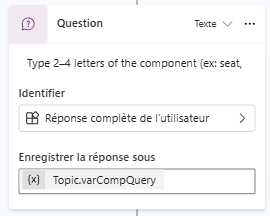
\includegraphics[width=0.4\textwidth]{images_pfe/Component input.png}
    \caption{Component input: User enters partial name; system prepares suggestion list.}
    \label{fig:component-input}
\end{figure}
\item \textbf{Show available roles}: For J4U, available roles are DRE, Pilot, CTE. Engineer confirms: ``Yes, DRE.''
    \begin{figure}[H]
    \centering
    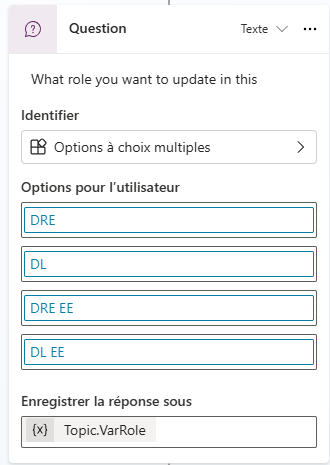
\includegraphics[width=0.4\textwidth]{images_pfe/question role.png}
    \caption{Role selection: User selects from available roles.}
    \label{fig:role-selection}
\end{figure}
\item \textbf{Confirm the change}: LEON prompts: Do you want to Update External mirrors (J4U) DRE from Jane Smith to John Doe? Yes or No
    \begin{figure}[H]
    \centering
    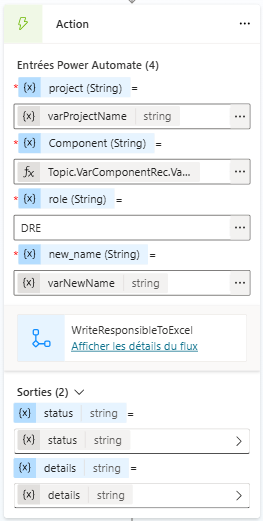
\includegraphics[width=0.35\textwidth]{images_pfe/update name1.png}
    \caption{Update execution: User confirms the assignment update.}
    \label{fig:update-execution}
\end{figure}
\item \textbf{Make the change}: Power Automate opens the Excel file, then it locates the cell (row External mirrors and column DRE in J4U) and writes John Doe in it, saves the file, and logs that modification.
    \begin{figure}[H]
    \centering
    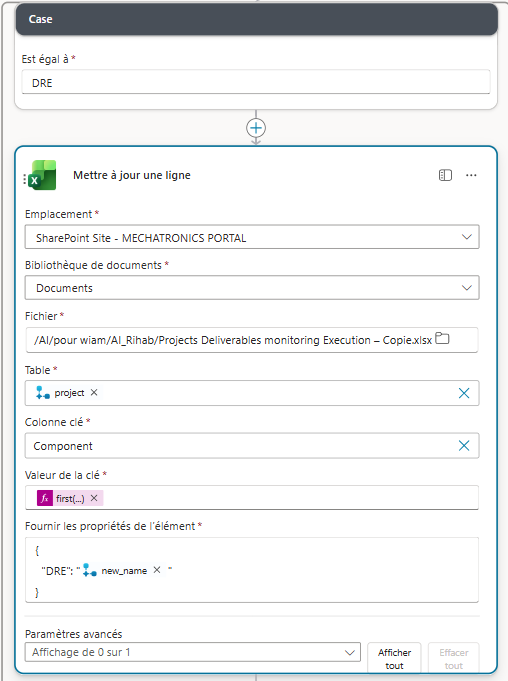
\includegraphics[width=0.4\textwidth]{images_pfe/update name2.png}
    \caption{Update execution: Cell value update in Excel.}
    \label{fig:update-write}
\end{figure}
\item \textbf{Confirm to user}: LEON confirms: ``Done. John Doe is now DRE for External mirrors in J4U.''
\end{enumerate}
\endgroup
\subsubsection{Error Handling}

What can go wrong when updating assignments:

\vspace{0.15cm}

\begin{tabularx}{0.95\textwidth}{|l|X|}
    \hline
    \textbf{What Happens} & \textbf{What LEON Does} \\
    \hline
    \texttt{PROJECT NOT FOUND} & Project name doesn't match any sheet. LEON suggests available projects. \\
    \hline
    \texttt{COMPONENT NOT FOUND} & Component doesn't exist in that project. LEON lists available components. \\
    \hline
    \texttt{ROLE NOT FOUND} & Role name doesn't exist in that project (e.g., CEO for J4U). LEON shows available roles. \\
    \hline
    \texttt{INVALID NEW NAME} & New name is empty or invalid. LEON asks: Who should be assigned? \\
    \hline
    \texttt{UNAUTHORIZED} & User lacks write permission on the Excel file. LEON says: You can't modify this assignment. \\
    \hline
    \texttt{DATASET UNAVAILABLE} & SharePoint is down or Excel file can't be accessed. LEON says: Can't access Excel right now. Try again later. \\
    \hline
    \texttt{WRITE FAILURE} & Excel write fails (file locked, quota exceeded). LEON escalates: Update failed. Contact IT. \\
    \hline
\end{tabularx}

\vspace{0.2cm}


\subsubsection{Output Format}

The response given by the Responsible Assignment Update service to the Copilot Studio at every attempt to update is presented as follows (see Figure~5.14).
 \begin{figure}[H]
    \centering
    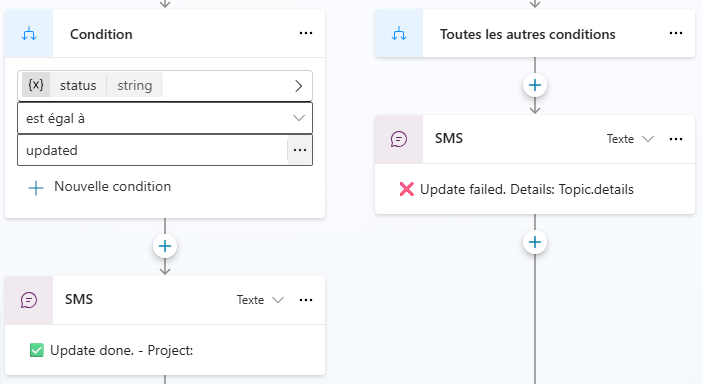
\includegraphics[width=0.4\textwidth]{images_pfe/update name.png}
    \caption{Update execution: Final confirmation and result to user.}
    \label{fig:update-result}
\end{figure}

\begin{itemize}
    \item[\quad\textbullet] \textbf{Success case}: 
The success path explicitly includes the step that the change was made while indicating the old responsible and the new one to be used during the process. The data returned consists of: \texttt{status=updated}, the \texttt{old responsible}, the \texttt{new responsible} and a timestamp in the ISO-8601 format. Copilot Studio presents a small confirmation message that summarizes the updated project, the component and the role to be affected by the update.
    \item[\quad\textbullet] \textbf{Error case}: 
    In the case of failure of update, the service will respond with error response where status will be with the error code (COMPONENT NOT FOUND, UNAUTHORIZED, etc.) and short details field. Copilot Studio will render a user friendly error message and present with the next action to perform (Retry with updated data, Specify, escalate...).
\end{itemize}





\subsection{\textcolor[HTML]{003D99}{Implementation: Send Notification and Email}}
\label{sec:impl-notification}

\subsubsection{Objective and Scope}

The Send Notification and Email service enables users to communicate with project stakeholders through structured email messages. The service supports two operational modes: (1) draft mode, where email messages are prepared for review without sending, and (2) send mode, where messages are immediately transmitted to recipients. The service integrates recipient resolution via Azure Active Directory (AAD) directory lookup, message composition via user input or predefined templates, and email transmission via the Microsoft Outlook connector. \textbf{All emails are user-generated or template-based;} the system does NOT perform autonomous message composition or AI-generated content. All email operations are logged for audit and compliance purposes.

\subsubsection{System Architecture}

The email service is implemented through the following integrated components:
 \begin{figure}[H]
    \centering
    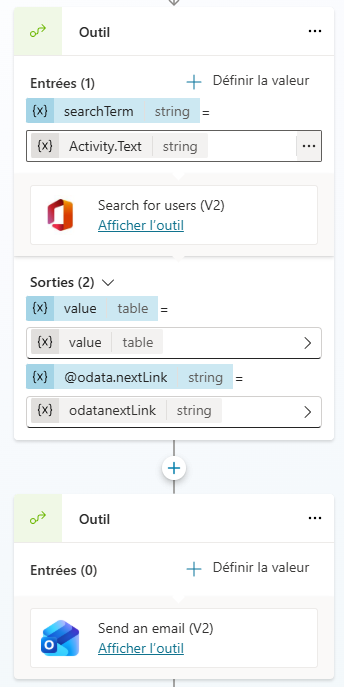
\includegraphics[width=0.4\textwidth]{images_pfe/email.png}
    \caption{Email service architecture overview.}
    \label{fig:email-architecture}
\end{figure}
\begin{itemize}
    \item[\quad\textbullet] \textbf{Copilot Studio}: Conversational interface for user intent detection and message orchestration.
    \item[\quad\textbullet] \textbf{Power Automate}: Workflow execution engine that coordinates recipient resolution, validation, and transmission.
    \item[\quad\textbullet] \textbf{Azure Active Directory (AAD) connector}: Provides user directory search via ``Search for users (V2)'' action for recipient resolution.
    \item[\quad\textbullet] \textbf{Microsoft Outlook connector}: Handles email transmission via [Company] mail service.
    \item[\quad\textbullet] \textbf{Copilot audit logs}: Records all email operations for compliance and traceability.
\end{itemize}

\subsubsection{Input Processing}

The email service accepts the following user inputs:
 \begin{figure}[H]
    \centering
    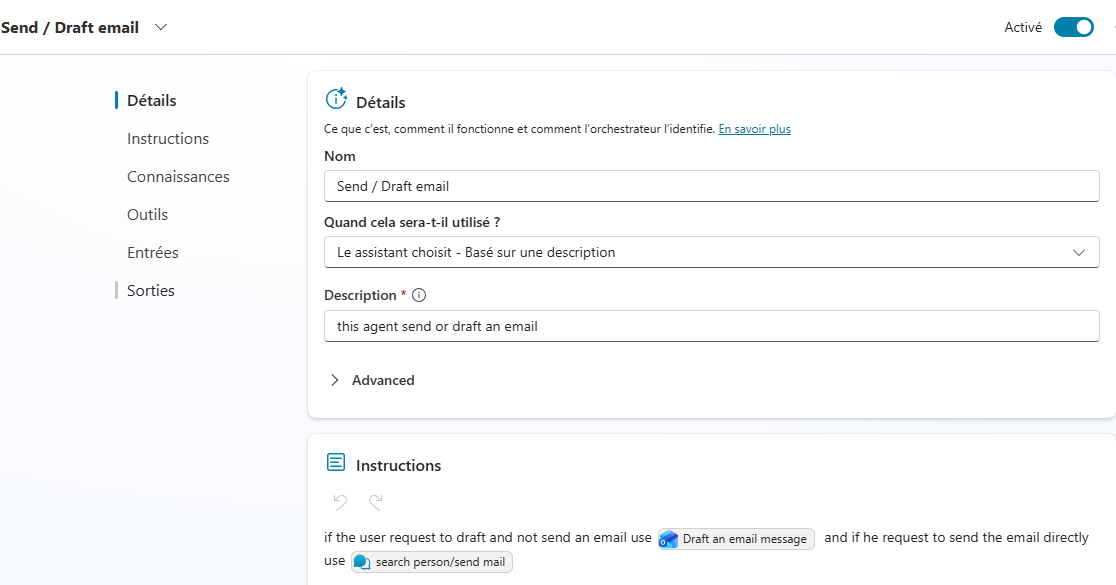
\includegraphics[width=0.4\textwidth]{images_pfe/email assistant.png}
    \caption{Email service architecture overview.}
    \label{fig:email-architecture}
\end{figure}
\noindent\fbox{%
    \parbox{0.95\textwidth}{%
        \textbf{User Input Parameters:}
        \begin{itemize}[leftmargin=0.3cm, itemsep=0.15cm]
            \item \textbf{Operation mode}: ``draft'' or ``send''
            \item \textbf{Recipient}: Name, email partial, or keyword for directory lookup
            \item \textbf{Subject}: Email subject line
            \item \textbf{Body}: Message content provided by user or selected from predefined templates
            \item \textbf{Context (optional)}: Project, component, or assignment reference for template variable substitution
        \end{itemize}
    }%
}

\vspace{0.2cm}

\noindent\textbf{Input Processing Steps:}

\begin{enumerate}
    \setlength{\itemsep}{0.1cm}
    \setlength{\leftmargin}{0.5cm}
    \item \textbf{Conversational capture}: User provides email request through Copilot Studio natural language interface. Example: ``Send an email to John Doe about component X4'', or ``Draft a message to the DRE responsible for this component.''
    \item \textbf{Intent detection}: Copilot NLU analyzes user utterance to determine:
    \begin{itemize}
        \setlength{\leftmargin}{0.7cm}
        \item Operation intent: draft or send
        \item Recipient specification (name, keyword, or role)
        \item Message content (subject, body, or template reference [à préciser])
    \end{itemize}
    \item \textbf{Validation}: System checks that required parameters (mode, recipient, subject, body) are provided. Missing inputs trigger Copilot clarification requests.
\end{enumerate}

\subsubsection{Recipient Resolution}

Recipient resolution is handled by the Power Automate ``Search for users (V2)'' action, which queries Azure Active Directory:

\begin{enumerate}
    \setlength{\itemsep}{0.1cm}
    \setlength{\leftmargin}{0.5cm}
    \item \textbf{User query input}: Recipient identifier from user (name, email partial, or keyword).
    \item \textbf{AAD directory search}: Power Automate invokes ``Search for users (V2)'' with the user query.
    \item \textbf{Match result processing}:
    \begin{itemize}
        \setlength{\leftmargin}{0.7cm}
        \item \textbf{Exact single match}: Recipient email address is extracted and confirmed.
        \item \textbf{Multiple matches}: Copilot presents matching users as a selectable list; user selects the correct recipient.
        \item \textbf{No matches}: Return \texttt{USER\_NOT\_FOUND}; Copilot requests clarification or alternative recipient specification.
    \end{itemize}
    \item \textbf{Email extraction}: Confirmed recipient email address is extracted and passed to the execution logic.
\end{enumerate}

\noindent This approach ensures that emails are sent to verified directory identities, reducing delivery failures and incorrect recipient issues.

\subsubsection{Execution Logic}

Once recipient and message parameters are confirmed, the system executes the email operation:

\vspace{0.15cm}

\noindent\textbf{Case A: Draft Mode (Prepare without Send)}

\begin{enumerate}
    \setlength{\itemsep}{0.1cm}
    \setlength{\leftmargin}{0.5cm}
    \item \textbf{Email composition}: System assembles email message with:
    \begin{itemize}
        \setlength{\leftmargin}{0.7cm}
        \item \texttt{to}: Recipient email address (resolved)
        \item \texttt{subject}: Subject line from user input
        \item \texttt{body}: Message body from user input or template [à préciser]
    \end{itemize}
    \item \textbf{No transmission}: Email draft is NOT sent; it is retained in-memory or stored in [à préciser: temporary location].
    \item \textbf{Draft preview}: System displays email preview to user for review:
    \begin{center}
        \textbf{From:} [System sender] \\
        \textbf{To:} [Recipient name] $<$[recipient@email.com]$>$ \\
        \textbf{Subject:} [Subject line] \\
        \rule[0.5ex]{\textwidth}{0.5pt} \\{}[Message body preview]
    \end{center}
    \item \textbf{User action}: User reviews draft and selects:
    \begin{itemize}
        \setlength{\leftmargin}{0.7cm}
        \item ``Send'' (transitions to Case B)
        \item ``Edit'' (return to input for modification)
        \item ``Cancel'' (discard draft)
    \end{itemize}
\end{enumerate}

\vspace{0.15cm}

\noindent\textbf{Case B: Send Mode (Direct Transmission)}

\begin{enumerate}
    \setlength{\itemsep}{0.1cm}
    \setlength{\leftmargin}{0.5cm}
    \item \textbf{Flow trigger}: Copilot invokes Power Automate flow ``Flow-Send-Email'' with parameters:
    \begin{itemize}
        \setlength{\leftmargin}{0.7cm}
        \item \texttt{recipient\_email}: Resolved email address from AAD lookup
        \item \texttt{subject}: Subject line
        \item \texttt{body}: Message body
        \item [à préciser: optional context fields for templated messages]
    \end{itemize}
    \item \textbf{Outlook connector invocation}: Power Automate calls Microsoft Outlook connector with email parameters.
    \item \textbf{Transmission}: Outlook connector sends email via [Company] mail service.
    \item \textbf{Delivery confirmation}: System receives confirmation from Outlook (success or failure status).
    \item \textbf{Audit logging}: Email send event is logged with full context (timestamp, sender, recipient, subject, delivery status).
\end{enumerate}

\noindent \textbf{Automated Email Triggers}

In addition to user-initiated email, Power Automate flows automatically trigger emails for specific events:

\begin{itemize}
    \item[\quad\textbullet] \textbf{Responsible assignment update}: Template-based confirmation email sent to old and new responsible persons when an assignment changes.
    \item[\quad\textbullet] \textbf{Workload assignment creation}: Template-based confirmation email sent to assigned actor with task details (component, project, hours, dates).
    \item[\quad\textbullet] \textbf{Gate progression}: Template-based notification sent when component reaches new gate level (planned enhancement).
\end{itemize}

\noindent Automated emails use predefined, static templates stored in the Copilot Studio knowledge base or SharePoint; content is populated by Power Automate using available context variables (project name, component name, actor name, dates). \textbf{No autonomous message generation is performed;} templates ensure compliance and consistency.

\subsubsection{Error Handling and Fallback}

The email service produces the following error conditions:

\vspace{0.15cm}

\begin{tabularx}{0.95\textwidth}{|l|X|}
    \hline
    \textbf{Error Code} & \textbf{Description and Response} \\
    \hline
    \texttt{USER\_NOT\_FOUND} & Recipient query does not match any AAD directory entry. Copilot requests clarification or alternative recipient name. \\
    \hline
    \texttt{AMBIGUOUS\_USER} & Multiple AAD users match the recipient query. Copilot presents list for user selection. \\
    \hline
    \texttt{MISSING\_SUBJECT} & Subject line is empty or not provided. Copilot requests subject from user. \\
    \hline
    \texttt{MISSING\_BODY} & Message body is empty or not provided. Copilot requests message content. \\
    \hline
    \texttt{INVALID\_EMAIL} & Recipient email address is malformed or invalid. System rejects and requests clarification. \\
    \hline
    \texttt{OUTLOOK\_UNAVAILABLE} & Outlook connector is unreachable or [Company] mail service is down. Power Automate logs attempt; Copilot notifies user and suggests retry. \\
    \hline
    \texttt{SEND\_FAILURE} & Email transmission fails for unspecified reason (quota, recipient blocking, network). Error details returned; Copilot escalates or suggests alternative contact method. \\
    \hline
    \texttt{UNAUTHORIZED} & User lacks permission to send emails or recipient is blocked from receiving external messages. Response: ``You do not have permission to send this email.'' Copilot escalates. \\
    \hline
\end{tabularx}

\vspace{0.2cm}

\noindent For any error, Copilot provides user-friendly feedback with suggested next steps (retry, escalation, manual intervention).


\subsubsection{Output Format}

The email service returns different outputs depending on operation mode:

\vspace{0.15cm}

\begin{itemize}
    \item[\quad\textbullet] \textbf{Draft mode output}:
    \begin{itemize}[leftmargin=0.5cm]
        \item Email preview displayed to user with sender, recipient, subject, and body
        \item Action prompts: ``Send'', ``Edit'', or ``Cancel''
        \item No email is transmitted until user confirms ``Send''
    \end{itemize}
    
    \item[\quad\textbullet] \textbf{Send mode success output}:
    \begin{itemize}[leftmargin=0.5cm]
        \item Conversational confirmation: ``Email successfully sent to [Recipient Name] $<$[recipient@email.com]$>$ with subject '[Subject]'. Sent at [ISO-8601 timestamp].''
        \item Audit record created automatically
    \end{itemize}
    
    \item[\quad\textbullet] \textbf{Send mode error output}:
    \begin{itemize}[leftmargin=0.5cm]
        \item Error code and description: ``Email send failed: [ERROR\_CODE]. [Human-readable message].''
        \item Suggested next steps: retry, escalate, or use alternative contact method
        \item Error logged to audit trail for investigation
    \end{itemize}
    
    \item[\quad\textbullet] \textbf{Automated email output}:
    \begin{itemize}[leftmargin=0.5cm]
        \item No user interface output; email sent silently in background
        \item Status recorded in Power Automate flow run history
        \item Audit entry created with ``AUTOMATED'' operation type flag
    \end{itemize}
\end{itemize}

% ─────────────────────────────────────────────────────────────────────────────
% ═════════════════════════════════════════════════════════════════════════════
\section{\textcolor[HTML]{0066CC}{SpecValidator Implementation}}
% ═════════════════════════════════════════════════════════════════════════════
\label{sec:impl-specvalidator}

SpecValidator is an independent, deterministic service implemented as an Azure Function. It executes specification validation logic in isolation, ensuring reproducibility and auditability. The output is a detailed validation report (no auto-fix).

\subsection{\textcolor[HTML]{003D99}{Function Architecture}}

\paragraph{Technology Stack}

\begin{itemize}
    \item \textbf{Runtime} : Azure Functions (.NET 6.0 or later, C\#).
    \item \textbf{Trigger} : HTTP trigger, invoked by Copilot Studio.
    \item \textbf{Authentication} : AAD service-to-service (Managed Identity).
\end{itemize}

\paragraph{Function Endpoint}

\begin{verbatim}
POST /api/validate-specification
Headers:
  Authorization: Bearer <AAD-token>
  Content-Type: application/json

Body:
{
  "specificationId": "[spec-id]",
  "projectId": "[project-id]",
  "componentId": "[component-id]",
  "gateLevel": "[Gate 1|Gate 2|Gate 3]",
  "specificationContent": "<file-content or URL>",
  "validationRuleSetId": "[rule-set-id]"
}

Response (200):
{
  "validationId": "[validation-id]",
  "specificationId": "[spec-id]",
  "timestamp": "[ISO-8601]",
  "status": "PASS | FAIL | WARN",
  "conformanceScore": 0.0--1.0,
  "issues": [
    {
      "severity": "ERROR | WARNING | INFO",
      "category": "[rule-category]",
      "message": "[human-readable message]",
      "location": "[line:col or section]"
    }
  ],
  "recommendations": ["[recommendation-1]", ...],
  "executionTime": "[milliseconds]"
}
\end{verbatim}

\subsection{\textcolor[HTML]{003D99}{Rule Storage and Versioning}}

\paragraph{Azure Blob Storage Structure}

\begin{verbatim}
/validation-rules/
  ├── gate-1/
  │   ├── rules-v1.0.json
  │   ├── rules-v1.1.json
  │   └── [current] -> rules-v1.1.json
  ├── gate-2/
  │   ├── rules-v1.0.json
  │   └── [current]
  ├── gate-3/
  └── [templates]/
      ├── spec-template-gate1.docx
      ├── spec-template-gate2.docx
\end{verbatim}

\paragraph{Rule File Format (JSON)}

\begin{verbatim}
{
  "ruleSetId": "[gate-N-rules-v1.x]",
  "version": "1.1",
  "lastModified": "[ISO-8601]",
  "description": "Validation rules for Gate N",
  "rules": [
    {
      "ruleId": "[rule-001]",
      "category": "[Structure|Content|Format]",
      "severity": "ERROR | WARNING | INFO",
      "description": "[rule description]",
      "pattern": "[regex or condition]",
      "message": "[error message]"
    }
  ]
}
\end{verbatim}

\subsection{\textcolor[HTML]{003D99}{Validation Pipeline}}

\begin{enumerate}
    \item \textbf{Input validation} : verify specificationId, projectId, gateLevel.
    \item \textbf{Fetch specification} : from request body or external URL.
    \item \textbf{Load applicable rules} : from Azure Blob Storage (based on gateLevel).
    \item \textbf{Execute rules} : apply each rule to specification content; record violations.
    \item \textbf{Calculate score} : (total rules - errors) / total rules.
    \item \textbf{Generate report} : list all issues, recommendations, execution time.
    \item \textbf{Log event} : record to Copilot audit and Power Automate.
    \item \textbf{Return response} : JSON with all validation details.
\end{enumerate}

\paragraph{Performance}

Target execution time: < 5 seconds for typical specifications.

\subsection{\textcolor[HTML]{003D99}{Output: Detailed Validation Report}}

\paragraph{Report Structure}

\begin{table}[H]
    \centering
    \small
    \caption{SpecValidator detailed validation report structure.}
    \label{tab:impl-specvalidator-report}
    \begin{tabularx}{\textwidth}{|l|X|}
        \hline
        \textbf{Field} & \textbf{Description} \\
        \hline
        validationId & Unique identifier for this validation run \\
        \hline
        specificationId & Reference to submitted specification \\
        \hline
        timestamp & When validation occurred \\
        \hline
        status & PASS / FAIL / WARN \\
        \hline
        conformanceScore & 0.0--1.0 percentage of rules satisfied \\
        \hline
        issues[].severity & ERROR / WARNING / INFO \\
        \hline
        issues[].message & Specific violation description \\
        \hline
        issues[].location & Where in specification (line, section) \\
        \hline
        recommendations[] & Suggested corrections or improvements \\
        \hline
        executionTime & Milliseconds to complete validation \\
        \hline
    \end{tabularx}
\end{table}

\paragraph{No Auto-Fix}

SpecValidator generates detailed reports with recommendations but does \textbf{NOT} automatically modify specifications. Users review findings and make corrections manually.

% ─────────────────────────────────────────────────────────────────────────────
% ═════════════════════════════════════════════════════════════════════════════
\section{\textcolor[HTML]{0066CC}{Cross-Cutting Concerns}}
% ═════════════════════════════════════════════════════════════════════════════
\label{sec:impl-crosscutting}

\subsection{\textcolor[HTML]{003D99}{Access Control Enforcement}}

\paragraph{Authentication}

\begin{itemize}
    \item \textcolor[HTML]{003D99}{\textbf{Copilot Studio agent}} : leverages [Company] Teams/AAD authentication.
    \item \textcolor[HTML]{003D99}{\textbf{Power Automate flows}} : use Service Principal (Managed Identity).
    \item \textcolor[HTML]{003D99}{\textbf{SpecValidator}} : authenticates via AAD token.
\end{itemize}

\paragraph{Authorization (RBAC)}

Enforced via AAD group membership:

\begin{table}[H]
    \centering
    \small
    \caption{RBAC matrix for LEON operations.}
    \label{tab:impl-rbac}
    \begin{tabularx}{\textwidth}{|l|l|X|}
        \hline
        \textbf{Operation} & \textbf{Required AAD Group} & \textbf{Description} \\
        \hline
        View Who-is-Who & [Company]-LEON-Users & All authenticated users \\
        \hline
        View Gate Status & [Company]-LEON-Users & All authenticated users \\
        \hline
        Update Responsible & [Company]-LEON-Governance-Admin & Governance team \\
        \hline
        Upload Deliverable & [Company]-LEON-Users & All authenticated users \\
        \hline
        Manage Workload & [Company]-LEON-Resource-Manager & Resource managers \\
        \hline
        Invoke SpecValidator & [Company]-LEON-Users & All authenticated users \\
        \hline
        View Audit Log & [Company]-LEON-Auditor & Compliance/audit teams \\
        \hline
    \end{tabularx}
\end{table}

\subsection{\textcolor[HTML]{003D99}{Logging and Audit}}

All LEON actions are logged via:

\begin{enumerate}
    \item \textcolor[HTML]{003D99}{\textbf{Copilot Studio audit logs}} : conversation history, user intents, topic flows.
    \item \textcolor[HTML]{003D99}{\textbf{Power Automate flow runs}} : flow execution status, inputs, outputs, start/end times.
    \item \textcolor[HTML]{003D99}{\textbf{Azure Functions logs}} : SpecValidator execution details (via Application Insights).
\end{enumerate}

\paragraph{Audit Trail Fields}

\begin{itemize}
    \item \textcolor[HTML]{003D99}{\textbf{Timestamp}} (ISO-8601)
    \item \textcolor[HTML]{003D99}{\textbf{User identity}} (AAD OID + email)
    \item \textcolor[HTML]{003D99}{\textbf{Action type}} (e.g., LOOKUP\_RESPONSIBLE, VALIDATE\_SPEC)
    \item \textcolor[HTML]{003D99}{\textbf{Resource affected}} (component, gate, specification)
    \item \textcolor[HTML]{003D99}{\textbf{Status}} (SUCCESS / FAILURE)
    \item \textcolor[HTML]{003D99}{\textbf{Result details}} (old/new values for updates)
    \item \textcolor[HTML]{003D99}{\textbf{Error message}} (if applicable)
\end{itemize}

\paragraph{Retention}

[à préciser: retention period, e.g., 7 years for compliance]

\subsection{\textcolor[HTML]{003D99}{Traceability Tags}}

Every artifact is tagged for traceability:

\begin{itemize}
    \item \textbf{Specification tag} : \texttt{spec-validation-[validation-id]} links spec to validation result.
    \item \textbf{Responsible update tag} : \texttt{responsible-change-[timestamp]} marks updates.
    \item \textbf{Gate progression tag} : \texttt{gate-transition-[gate-id]-[timestamp]} tracks status changes.
\end{itemize}

% ─────────────────────────────────────────────────────────────────────────────
% ═════════════════════════════════════════════════════════════════════════════
\section{\textcolor[HTML]{0066CC}{Summary of Implemented Artifacts}}
% ═════════════════════════════════════════════════════════════════════════════
\label{sec:impl-summary}

\subsection{\textcolor[HTML]{003D99}{Copilot Studio Topics}}

\begin{table}[H]
    \centering
    \small
    \caption{Summary of Copilot Studio topics and associated flows.}
    \label{tab:impl-topics}
    \begin{tabularx}{\textwidth}{|l|X|l|}
        \hline
        \textbf{Topic Name} & \textbf{User Intent} & \textbf{Triggered Flow} \\
        \hline
        Who-is-Who Search & Find responsible party & Flow-WhoIsWho-Lookup \\
        \hline
        Gate Status & Get gate information & Flow-Gate-Status-Retrieve \\
        \hline
        Update Responsible & Modify responsible (RBAC gated) & Flow-Responsible-Update \\
        \hline
        Upload Deliverable & Submit file to gate & Flow-Upload-to-Gate \\
        \hline
        Workload Management & View/update assignments & Flow-Workload-View / Update \\
        \hline
        Send Notification & Trigger email & Flow-Send-Email \\
        \hline
        Escalate & Unresolved query & Human support handoff \\
        \hline
    \end{tabularx}
\end{table}

\subsection{\textcolor[HTML]{003D99}{Power Automate Flows (6--7 Primary)}}

\begin{table}[H]
    \centering
    \small
    \caption{Summary of primary Power Automate workflows.}
    \label{tab:impl-pa-flows}
    \begin{tabularx}{\textwidth}{|l|X|}
        \hline
        \textbf{Flow Name} & \textbf{Key Actions} \\
        \hline
        Flow-WhoIsWho-Lookup & Query [SharePoint], return responsible party \\
        \hline
        Flow-Gate-Status-Retrieve & Query gate metadata, return timeline \\
        \hline
        Flow-Responsible-Update & Update [SharePoint], log audit, notify \\
        \hline
        Flow-Upload-to-Gate & Create [SharePoint] path, upload file, log \\
        \hline
        Flow-Workload-View & Query assignments, return summary \\
        \hline
        Flow-Workload-Update & Insert/update assignment, log, notify \\
        \hline
        Flow-Send-Email & Send via Outlook, log delivery \\
        \hline
    \end{tabularx}
\end{table}

\subsection{\textcolor[HTML]{003D99}{SpecValidator Configuration}}

\begin{itemize}
    \item \textbf{Function App} : \texttt{[Company]-SpecValidator-Func}
    \item \textbf{Function} : \texttt{ValidateSpecification} (HTTP-triggered)
    \item \textbf{Runtime} : .NET 6.0, C\#
    \item \textbf{Managed Identity} : enabled for Azure Blob Storage and audit logging
    \item \textbf{Application Settings} :
    \begin{itemize}
        \item \texttt{AzureStorageConnectionString} : Blob Storage for rule files
        \item \texttt{RuleCacheTTL} : [à préciser: cache duration, e.g., 3600 seconds]
    \end{itemize}
\end{itemize}

\subsection{\textcolor[HTML]{003D99}{5.6.4 Validation Rule Sets (Azure Blob Storage)}}

\begin{itemize}
    \item \textbf{Gate 1 rules} : v1.1 (current) - [à préciser: number of rules]
    \item \textbf{Gate 2 rules} : v1.0 (current) - [à préciser: number of rules]
    \item \textbf{Gate 3 rules} : v1.0 (current) - [à préciser: number of rules]
    \item \textbf{Specification templates} : stored for reference per gate level
\end{itemize}

\subsection{\textcolor[HTML]{003D99}{5.6.5 Copilot Studio Knowledge Base}}

\begin{itemize}
    \item \textbf{Structure} : Unified knowledge base housing all dataset files and connectors for LEON.
    \item \textbf{Who-is-Who dataset} : Excel file uploaded to KB with responsible party mappings (columns: [Project], [Component], [Responsible Name], [Responsible Email], [Role]).
    \item \textbf{Gate metadata} : Excel file in KB with gate timelines, owners, status, entry/exit dates.
    \item \textbf{Workload assignments} : Excel file in KB with task assignments, hours, deadlines.
    \item \textbf{Validation guidelines} : Word document (uploaded to KB) describing acceptance criteria per gate level.
    \item \textbf{[SharePoint] connectors} : real-time live connectors to [SharePoint] lists for current data; KB serves as cached reference for faster queries.
    \item \textbf{Update frequency} : [à préciser: daily, weekly, or on-demand manual sync from [SharePoint] to KB?]
\end{itemize}



% ─────────────────────────────────────────────────────────────────────────────
% ═════════════════════════════════════════════════════════════════════════════
\section{\textcolor[HTML]{0066CC}{Testing and Validation Approach}}
% ═════════════════════════════════════════════════════════════════════════════
\label{sec:impl-testing}

\subsection{\textcolor[HTML]{003D99}{5.7.1 Copilot Studio Prompt-Based Testing}}

Testing was conducted by executing test prompts directly in Copilot Studio and validating the information flow through topics and Power Automate flows.

\paragraph{Test Methodology}

\begin{enumerate}
    \item \textbf{Prompt design} : craft natural language test scenarios representing each use case.
    \item \textbf{Execution} : submit prompts to Copilot agent in Test environment.
    \item \textbf{Observation} : monitor topic activation, flow triggering, inputs/outputs.
    \item \textbf{Validation} : verify correct data retrieval, transformations, and response generation.
    \item \textbf{Logging} : review Copilot logs and Power Automate flow runs to trace execution path.
\end{enumerate}

\paragraph{Test Coverage}

Beta testing was conducted with approximately 15 users from the mechatronics and governance teams. Testers executed natural language prompts across all major use cases (Who-is-Who lookup, Gate status, Upload, Workload, SpecValidator) and provided feedback on conversational quality, information accuracy, and flow execution. Detailed feedback notes were collected and reviewed post-testing.

Test scenarios include:

\begin{enumerate}
    \item \textcolor[HTML]{003D99}{\textbf{Who-is-Who lookup}} : valid and invalid component/project combinations.
    \item \textcolor[HTML]{003D99}{\textbf{Gate status retrieval}} : existing and non-existent gates.
    \item \textcolor[HTML]{003D99}{\textbf{Responsible update}} : authorized and unauthorized users.
    \item \textcolor[HTML]{003D99}{\textbf{File upload}} : valid and invalid file formats [à préciser: which formats?].
    \item \textcolor[HTML]{003D99}{\textbf{Workload management}} : view and update operations.
    \item \textcolor[HTML]{003D99}{\textbf{SpecValidator invocation}} : passing and failing specifications.
    \item \textcolor[HTML]{003D99}{\textbf{Error scenarios}} : missing data, service unavailability, malformed input.
\end{enumerate}

\subsection{\textcolor[HTML]{003D99}{5.7.2 Traceability: Testing to Strategic Objectives}}

Testing aligned with strategic objectives:

\begin{table}[H]
    \centering
    \small
    \caption{Test scenarios mapped to strategic objectives.}
    \label{tab:impl-test-mapping}
    \begin{tabularx}{\textwidth}{|l|l|c|}
        \hline
        \textbf{SO} & \textbf{Test Scenario Type} & \textbf{Covered?} \\
        \hline
        SO1 & Conversational intent → topic → flow execution & [à préciser: Yes/No] \\
        \hline
        SO2 & Who-is-Who lookup accuracy and performance & [à préciser: Yes/No] \\
        \hline
        SO3 & Gate status retrieval and live updates & [à préciser: Yes/No] \\
        \hline
        SO4 & SpecValidator determinism and report quality & [à préciser: Yes/No] \\
        \hline
        SO5 & Audit trail completeness and accessibility & [à préciser: Yes/No] \\
        \hline
    \end{tabularx}
\end{table}

\subsection{\textcolor[HTML]{003D99}{5.7.3 Known Limitations and Future Work}}

\begin{enumerate}
    \item \textcolor[HTML]{003D99}{\textbf{Knowledge base synchronization lag}} : Copilot KB is a cached copy of [SharePoint] data. Updates to Who-is-Who or Gate metadata in [SharePoint] may take [à préciser: e.g., 1--4 hours] to reflect in the KB. For time-critical queries, Power Automate flows query [SharePoint] directly to fetch live data, mitigating this delay for most use cases. Future: implement automated KB refresh triggers.
    \item \textcolor[HTML]{003D99}{\textbf{Natural language understanding edge cases}} : Some user queries with ambiguous phrasing or typos may not be recognized by Copilot NLU, causing topic mismatch or escalation to human support. Mitigation: ongoing training of NLU model with real user interactions; escalation workflow ensures queries are not lost.
    \item \textcolor[HTML]{003D99}{\textbf{File upload format enforcement}} : While the system accepts Excel and Word files, very large files (>50 MB) or corrupted files may cause upload failures. Future: implement pre-upload validation and file compression.
    \item \textcolor[HTML]{003D99}{\textbf{SpecValidator rule versioning}} : Rule updates in Azure Blob Storage require manual version management. No automated rollback if a new rule set introduces false positives. Future: implement A/B testing framework for rule sets before promoting to production.
    \item \textcolor[HTML]{003D99}{\textbf{Audit log retention policy}} : [à préciser: Define retention period (e.g., 7 years for compliance). Implement automated archival to cold storage after retention threshold.]
\end{enumerate}

% ─────────────────────────────────────────────────────────────────────────────
% ═════════════════════════════════════════════════════════════════════════════
\section{\textcolor[HTML]{0066CC}{Deployment and Change Management}}
% ═════════════════════════════════════════════════════════════════════════════
\label{sec:impl-deployment}

\subsection{\textcolor[HTML]{003D99}{5.8.1 Deployment Timeline}}

\begin{table}[H]
    \centering
    \small
    \caption{Deployment phases and timeline.}
    \label{tab:impl-deployment-phases}
    \begin{tabularx}{\textwidth}{|l|X|X|}
        \hline
        \textbf{Phase} & \textbf{Scope} & \textbf{Date / Status} \\
        \hline
        Development (Dev) & Prototype and configuration & [à préciser] \\
        \hline
        Testing (Test) & UAT and scenario validation & [à préciser] \\
        \hline
        Pilot (Prod) & [à préciser: e.g., 2 projects, 50 users] & [à préciser] \\
        \hline
        Full Rollout (Prod) & All projects and users & [à préciser] \\
        \hline
    \end{tabularx}
\end{table}

\subsection{\textcolor[HTML]{003D99}{5.8.2 User Training and Support}}

\begin{itemize}
    \item \textcolor[HTML]{003D99}{\textbf{Training materials}} : [à préciser: documentation, video, live sessions?]
    \item \textcolor[HTML]{003D99}{\textbf{Support channel}} : [Company]-LEON-Support team or [à préciser: helpdesk ticket queue?]
    \item \textcolor[HTML]{003D99}{\textbf{Post-deployment monitoring}} : [à préciser: metrics, SLA, escalation process?]
\end{itemize}

% ─────────────────────────────────────────────────────────────────────────────
% ═════════════════════════════════════════════════════════════════════════════
\section{\textcolor[HTML]{0066CC}{Chapter Conclusion}}
% ═════════════════════════════════════════════════════════════════════════════
\label{sec:impl-conclusion}

The implementation of LEON realizes the design architecture through a modular, cloud-native approach grounded in Copilot Studio's topic-based orchestration. The integration of conversational AI, Power Automate workflows, and deterministic validation services creates a flexible yet compliant governance platform.

Key achievements:

\begin{enumerate}
    \item \textcolor[HTML]{003D99}{\textbf{Conversational accessibility}} : users interact naturally with governance data via Copilot topics.
    \item \textcolor[HTML]{003D99}{\textbf{Modular design}} : governance services decoupled through Power Automate flows and reusable topics.
    \item \textcolor[HTML]{003D99}{\textbf{Deterministic validation}} : SpecValidator operates independently, ensuring reproducible and auditable results.
    \item \textcolor[HTML]{003D99}{\textbf{Multi-environment support}} : Dev, Test, and Production environments enable safe rollout and iteration.
    \item \textcolor[HTML]{003D99}{\textbf{Complete audit trail}} : all actions logged via Copilot Studio, Power Automate, and Azure Functions, enabling compliance verification.
\end{enumerate}

The validation approach—prompt-based testing within Copilot Studio—directly verifies the conversational experience and information flow, ensuring fidelity to the design specification.

% ═════════════════════════════════════════════════════════════════════════════









% ═════════════════════════════════════════════════════════════════════════════
% CHAPTER: Results and Evaluation
% ═════════════════════════════════════════════════════════════════════════════

\chapter{Validation, Testing and Results}
\label{chap:results}

% ═════════════════════════════════════════════════════════════════════════════
\section{\textcolor[HTML]{0066CC}{Validation Scope and Approach}}
% ═════════════════════════════════════════════════════════════════════════════

In this chapter we demonstrate the validation approach which was maintained on the LEON prototype once implementation phase was achieved. Our goal is not to state a production deployment but to demonstrate how the services which was implemented were tested and what was really measured during all tests and how these measured enable to reach objectives of the project.

This prototype was largely tested in the \textbf{Copilot Studio test pane}, which serves as the execution test part for the conversational layer. When the test pane is run, the dialogue flow is triggered through the Copilot Studio interface, and through Power Automate business logic is implemented to pull data from the SharePoint/Excel data stores in the same way it was defined in Chapter~\ref{chap:implementation}. The final end user channel will be \textbf{Teams / Microsoft 365 Copilot}, but only the prototype level test is reported at this chapter, assuming the final channel has not yet been deployed to production.

The validation was then carried out along 3 orthogonal axes : the nominal functional use cases were executed for each of the main services, the error conditions were checked, to make sure LEON will favor clarification, graceful fallback or denial instead of failure in silent mode, the access-controlled operations were browsed, from a RBAC point of view, especially regarding read/write on the governance data. To illustrate, if asked “Who owns the External mirrors in J4U?”, it should answer from the Excel file containing the information”, instead of providing a textual free format output. Or, if asked for the gate of a certain component which has no recorded port, since no catalogue entry was created for it, simply says that it diesn't exist in the recorded gate informations.

At this stage, the chapter makes no quantitative claims which have not been formally calculated. There are no numbers, for latency, the number of requests, or the number of statistical errors. The validation is done through scenarios end-to-end(user query $\rightarrow$ workflow execution $\rightarrow$ data access $\rightarrow$ response), with execution traces (e.g. workflow run history) and typical error handling examples.
% ═════════════════════════════════════════════════════════════════════════════
\section{\textcolor[HTML]{0066CC}{Functional Test Scenarios}}
% ═════════════════════════════════════════════════════════════════════════════

The functional campaign is based on some typical users requests that can be grouped to the basic services implemented in LEON. Table~\ref{tab:functional-validation-scenarios} summarizes some typical scenarios, their preconditions and their resulting behavior on the prototype.

\begin{table}[H]
\centering
\footnotesize
\renewcommand{\arraystretch}{1.25}
\caption{Representative functional test scenarios used for LEON prototype validation.}
\label{tab:functional-validation-scenarios}
\begin{tabularx}{\textwidth}{|p{0.9cm}|p{2.9cm}|p{2.6cm}|X|X|p{1.8cm}|}
\hline
\rowcolor[HTML]{E6F2FF}\textcolor[HTML]{003D99}{\textbf{ID}} & \textcolor[HTML]{003D99}{\textbf{User request}} & \textcolor[HTML]{003D99}{\textbf{Preconditions}} & \textcolor[HTML]{003D99}{\textbf{Expected result}} & \textcolor[HTML]{003D99}{\textbf{Obtained result}} & \textcolor[HTML]{003D99}{\textbf{Status}} \\
\hline
FT-01 & ``Who is responsible for Brake System in J4U?'' & The project sheet can be found within the Who-is-Who workbook, the component line and role column are carried out. & LEON recognizes project sheet and computes component/role pair and return the responsible person from Excel. & In the prototype path the conversational answer is transmitted following that the Excel source and the governance owner have read from the work book structure Figure~\ref{fig:w1-dataset-structure}. & Validated \\
\hline
FT-02 & ``What is the current gate for Suspension System in J4U?'' & The gate repositories are located in SharePoint; there are a lot of components stored within gates in SharePoint. & LEON will read through the recorded gate repositories and report the highest gate achieved by the component. & The reply we get depends on whether there are files present in gate folders ,see lookup logic Figure~\ref{fig:gate-detection-workflow}. & Validated \\
\hline
FT-03 & ``Update the DRE for External mirrors in J4U to John Doe.'' & User has permission to change the source workbook; project, component and role can be resolved. & LEON sends a confirmation request, the target cells will then be configured in Power Automate and an explicit message is sent back for confirmation. & The prototype flow illustrates the step through a clean update and concludes with a message that the write operation as demonstrated in Figures~\ref{fig:update-execution} and ~\ref{fig:update-write}. & Validated \\
\hline
FT-04 & ``Send a reminder to the responsible engineer for Brake System.'' & Recipient can be looked up from directory data; available subject/body or template data available. & The LEON resolves the recipient, create the message payload, send the notification/ draft path without exiting the conversational flow. & The prototype behavior we will focus on is the email capture and recipient resolution path illustrated in Figure~\ref{fig:email-assistant-flow}. & Validated \\
\hline
FT-05 & ``Validate this specification against the configured rules.'' & SpecValidator possesses a specification document and a collection of related rules. & Validator runs in a non-mutable and deterministic way and produce a structure of validation result. & The prototype was designed to enable a defined execution of rules and the production of a report. & Partially documented \\
\hline
\end{tabularx}
\end{table}

The selected scenarios reflect the primary value offered to the end-users of the prototype: access information on governance, read project maturity using documented evidence, amend the controlled information, send context aware communication and check the specifications using deterministic rules.\\
\noindent\textbf{Confidentiality note.} All screen captures contained within this chapter are disguised examples. All names, e-mail accounts, internal ids, share point URLs, housing paths will need to be obscured for the jury copy.

\begingroup
\setlength{\intextsep}{6pt}
\setlength{\textfloatsep}{6pt}
\setlength{\floatsep}{6pt}
\captionsetup[figure]{skip=4pt}

\subsection{\textcolor[HTML]{003D99}{Who-is-Who Scenario Evidence}}

The Who-is-Who test sequence was tested in a live lookup path: user requests the name of a responsible on a specific project and component, and the conversational layer identifies the project context and the backend logic to route the request to the governance dataset. The actual feasibility of this scenario depends on two observable aspects: the assistance being aware of the name of the project entered by the user and the orchestration managing the lookup or redirect when the expected record does not exist.
\begin{figure}[H]
\centering
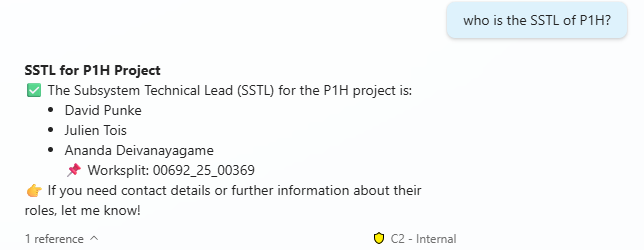
\includegraphics[width=0.8\textwidth]{images_pfe/who is who1.png}
\caption{Anonymized Copilot Studio capture used to support project disambiguation during the Who-is-Who validation path.}
\label{fig:results-who-conversation}
\end{figure}

\subsection{\textcolor[HTML]{003D99}{Gate Status Scenario Evidence}}

For gate status retrieval, the evidence needed to support the argument that the assistant searches through documents as opposed guessing at runtime via conversational utterance. Copilot Studio knowledge configuration is used for gate reasoning as a visual evidence, and the gate interpretation rule as an other visual evidence for highest documented maturity level return.


\subsection{\textcolor[HTML]{003D99}{Responsible Update Scenario Evidence}}

The update case is the most sensitive function path because it combines user input, authorization, write, and confirmation. The first proof here is regarding to conversation input state where user supply the real component fragment to go on the update procedure. The second proof shows the backend action‘s signature in order to supply update parameters to flow.



\subsection{\textcolor[HTML]{003D99}{Email and Notification Scenario Evidence}}

The use case was proved with the help of request path where LEON receives necessary inputs from the user intent, determines the recipient through directory connector, prepares delivery for the action message. Critical issues highlighted are on controlled execution such as before completing the input values it should not be delivering a notification.

\begin{figure}[H]
\centering
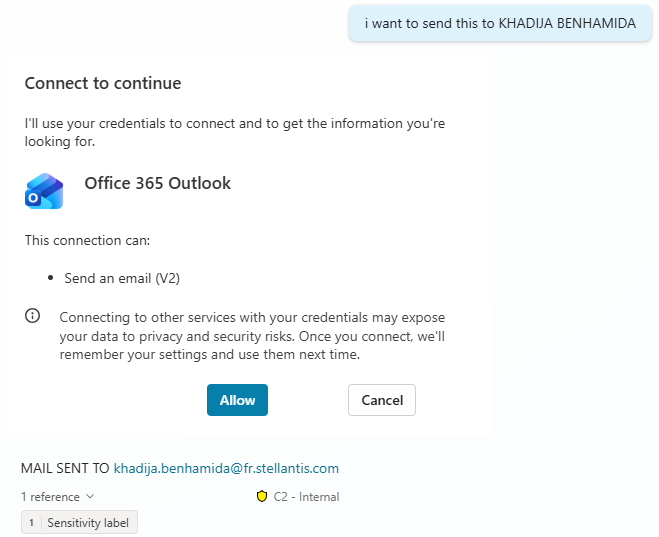
\includegraphics[width=0.72\textwidth]{images_pfe/email1.png}
\caption{Anonymized conversational capture used during e-mail and notification validation for request capture and field completion.}
\label{fig:results-email-conversation}
\end{figure}

\begin{figure}[H]
\centering
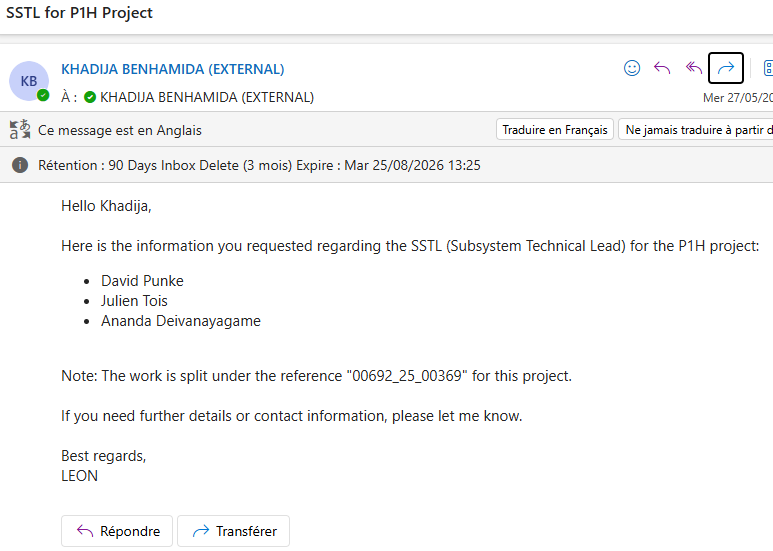
\includegraphics[width=0.42\textwidth]{images_pfe/email2.png}
\caption{Anonymized backend connector capture showing the notification path through recipient lookup and e-mail sending actions.}
\label{fig:results-email-flow}
\end{figure}
\begin{figure}[H]
\centering
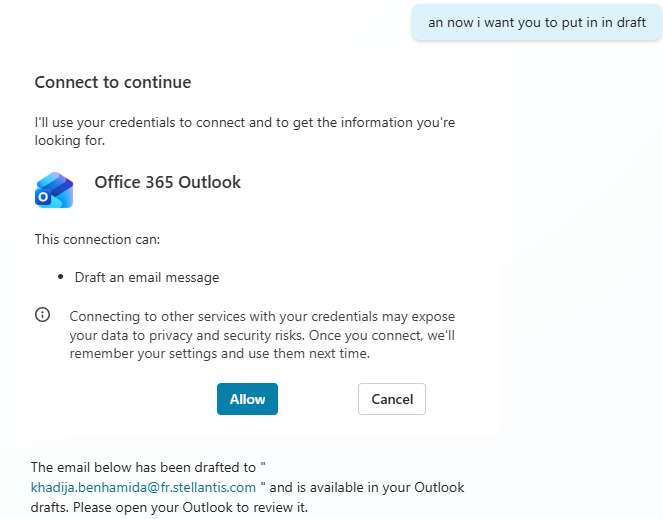
\includegraphics[width=0.72\textwidth]{images_pfe/email3.png}
\caption{Anonymized conversational capture used during e-mail and notification validation for request capture and field completion.}
\label{fig:results-email-conversation}
\end{figure}

\begin{figure}[H]
\centering
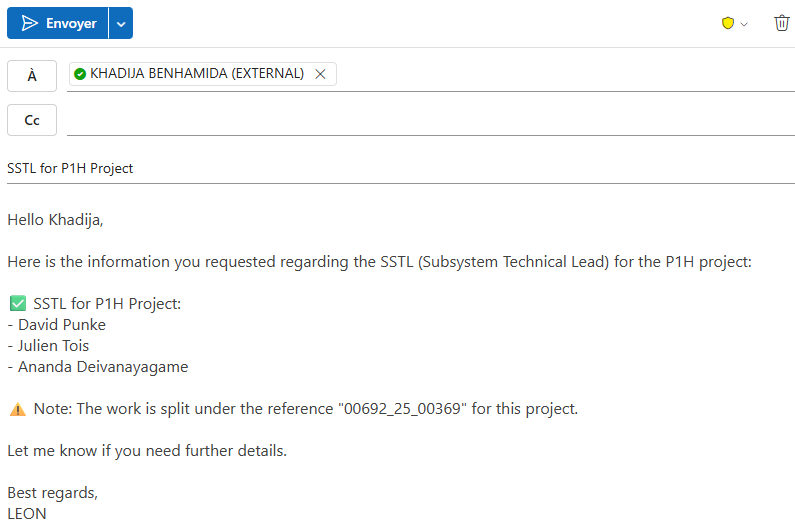
\includegraphics[width=0.42\textwidth]{images_pfe/email4.png}
\caption{Anonymized backend connector capture showing the notification path through recipient lookup and e-mail sending actions.}
\label{fig:results-email-flow}
\end{figure}
\subsection{\textcolor[HTML]{003D99}{SpecValidator Scenario Evidence}}

The SpecValidator path is less conversational than the governance services, but it still begins from the same prototype entry point. In the current working set of screenshots, the available evidence shows the test environment used to launch the scenario and the validation backend that executes deterministic checks. A dedicated anonymized test-pane capture of the exact validation request would remain preferable in a final defended version.



% ═════════════════════════════════════════════════════════════════════════════
\section{\textcolor[HTML]{0066CC}{Error and Robustness Testing}}
% ═════════════════════════════════════════════════════════════════════════════

It appeared that a nominal execution with general nominality execution was insufficient for a governance assistant. In fact, in real execution, the prototype also had to manage implicit cases where the user did not finish his request, or the asked entity or the backend source could be inaccessible. So robustness tests aimed at explicit error paths already modeled in implementation.
\begin{table}[H]
\centering
\footnotesize
\renewcommand{\arraystretch}{1.25}
\caption{Error and robustness scenarios checked during prototype validation.}
\label{tab:robustness-validation-scenarios}
\begin{tabularx}{\textwidth}{|p{3cm}|p{2.7cm}|X|p{2.2cm}|}
\hline
\rowcolor[HTML]{E6F2FF}\textcolor[HTML]{003D99}{\textbf{Error code}} & \textcolor[HTML]{003D99}{\textbf{Typical trigger}} & \textcolor[HTML]{003D99}{\textbf{Expected prototype behavior}} & \textcolor[HTML]{003D99}{\textbf{Control mode}} \\
\hline
\texttt{PROJECT NOT FOUND} & Unknown or misspelled project name & LEON does not quietly guess. It either asks a question or guesses the nearest known project name if there is a reasonable default option. & Clarification \\
\hline
\texttt{COMPONENT NOT FOUND} & Missing component from Excel sheet or file store & LEON interrupts the nominal path and asks user to give a better component name instead of providing an invalid result. & Clarification \\
\hline
\texttt{ROLE NOT FOUND} & The selected project has no specified roles & Indicates that the role is not present in the current context and then suggests available roles. & Clarification \\
\hline
\texttt{UNAUTHORIZED} & User attempts to read/write but lacks inherited privilege & The flow must stop, the backend execution must be visible on the refusal path and  the user must receive a clear authorization message. & Refusal / escalation \\
\hline
\texttt{DATASET UNAVAILABLE} & SharePoint, Excel or any other backend connector is currently down & LEON responds that the request cannot be serviced at the present time and recommends retrying or escalating. & Fallback \\
\hline
\end{tabularx}s
\end{table}

The validation rule remains the same: Any implicit or undeclared situation must be mapped to an explicit control flow on the conversation. For example a non-existing component name would then raise a reformulate request. A permission failure would prevent the action from performing and leave a history mark on the backend execution history.


% ═════════════════════════════════════════════════════════════════════════════
\section{\textcolor[HTML]{0066CC}{Security Validation and RBAC Review}}
% ═════════════════════════════════════════════════════════════════════════════

The review of RBAC was not made by non specified implicit internal rules but by testable empirical behaviors of the system. With LEON, there is no re-definition of the enterprise permissions: they are inherited from the access rights for the linked repository or connectors. This is an important aspect for governance, as the same conversational query can result in read success, write success, and deny based on the access rights on the SharePoint or the Excel sheet.\\

Two types of case are considered in validation: \textbf{authorization} or \textbf{non-authorization} cases. If the case is an authorization, then the request is authorized, the workflow proceeds as expected, and data is read or written. If the case is a non-authorization, then the request will not even reach a hidden workaround. The action is denied and a clear message appears to the user. The execution back-path can be visualized through the “Power Automate” run history. Realistically, someone with write access to a responsibility assignment should see the update process, while someone without it should have the flow blocked by an authorization message rather than a partial, hidden, or invisible modification.\\
The full proof of the this security test is (1) \textbf{the client message stating the permission} is allowed or denied to the end-user and (2) the \textbf{flow trace} proving if Power Automate flowed through the flow or not, and (3) \textbf{the modification side effect} to the source data if it were not to be changed at all. There is enough information to guarantee the RBAC prototype as it prove that we effect on the execution path and not only on the words displayed to the user.
\begin{table}[H]
\centering
\footnotesize
\renewcommand{\arraystretch}{1.25}
\caption{RBAC-oriented comparison between authorized and non-authorized prototype behaviors.}
\label{tab:rbac-validation-cases}
\begin{tabularx}{\textwidth}{|p{2.7cm}|p{2.6cm}|X|X|}
\hline
\rowcolor[HTML]{E6F2FF}\textcolor[HTML]{003D99}{\textbf{Case}} & \textcolor[HTML]{003D99}{\textbf{Example action}} & \textcolor[HTML]{003D99}{\textbf{Expected evidence}} & \textcolor[HTML]{003D99}{\textbf{Observed prototype behavior}} \\
\hline
Authorized & Inherit write permission to update the assignment & The conversational confirmation with the desired outcome the successful completion of a backend path with the expected data change is reflected in source workbook. & Update path finishes and returns success in explicit mode after flow receives the parameters \\
\hline
Non-authorized & Test with the same change that demands authorization to continue & Direct refusal message,  source data remains unchanged. & The guarded branch passes on a failure/refuse path rather than hidden or partial change. \\
\hline
\end{tabularx}
\end{table}


\endgroup

% ═════════════════════════════════════════════════════════════════════════════
\section{\textcolor[HTML]{0066CC}{Results and Technical Observations}}
% ═════════════════════════════════════════════════════════════════════════════

The validation work demonstrate that the prototype is actually executing all the main governance scenarios along an end-to-end chain, starting from the request input in Copilot Studio, moving through the Conversational Topic structure, up to Power Automate execution and resolution with enterprise data source and validation rules.There is no question of performance, it‘s more about the coherence between the user request and the back-end answer.

The below technical notes have been derived from tests and also from reviewing implemented flows:

\begin{itemize}
	\item The better the quality of source repositories, the better the answer will be to the governance questions. Naming inconsistencies between Excel sheets cause difficulty for matches even in the off-branch Whose-is-Who service which has naming normalization and fallback to default source when fails.
	\item The retrieval of gate status should rely on how well documents are organized in the gate repositories. In the case where a deliverable may be missing, in the wrong directory, or not yet available, LEON should assign no evidence to that state of maturity.
	\item Update service is more sensitive than read-only query due to interpretation, authorization, authorization and write execution, therefore, positive acknowledgment and traceability is important even in prototype.
	\item Email/notification functionalities are presented as enterprise features rather than general text-generation. Receiver resolution, quality of message and connector availability of mail box determine whether the request will be delivered to delivery, refinement or rejection.
	\item SpecValidator is the most deterministic of the block in the architecture, because its output is driven by a fixed document of rules applied to a fixed input, and not by the nuances of dialogue, therefore it provides a very suitable method for repeatable checking of compliance, given that the rules are explicitly version controlled, as are the inputs.
\end{itemize}

Based on all the above findings and conclusions, we can see that the prototype is working as expected, but we should still consider as a proved up to prototype, not an industrialized service deliver. The Copilot Studio Test pane is good for a proof of behavior and integration logic, but cannot replace a full operational system on the actual end-user channel.
% ═════════════════════════════════════════════════════════════════════════════
\section{\textcolor[HTML]{0066CC}{Synthesis Against Project Objectives (SO1..SO5)}}
% ═════════════════════════════════════════════════════════════════════════════

The final section of the validation chapter relates back to the sub-objectives defined earlier in this report. Table~\ref{tab:results-vs-objectives} pulls these together without overstating what has, and has not, been demonstrated by prototype.

\begin{table}[H]
\centering
\footnotesize
\renewcommand{\arraystretch}{1.25}
\caption{Synthesis of validation results against project objectives SO1 to SO5.}
\label{tab:results-vs-objectives}
\begin{tabularx}{\textwidth}{|p{2.5cm}|X|p{2.5cm}|}
\hline
\rowcolor[HTML]{E6F2FF}\textcolor[HTML]{003D99}{\textbf{Objective}} & \textcolor[HTML]{003D99}{\textbf{Validation evidence}} & \textcolor[HTML]{003D99}{\textbf{Assessment}} \\
\hline
SO1 -- Who-is-Who Lookup & This target is covered by scenario FT-01 as well as the workbook structure in Figure~\ref{fig:w1-dataset-structure}, lookup path in Figure~\ref{fig:w4-lookup}, and the explicit fallback as in Figure~\ref{fig:w5-error-condition}.  From this it can be seen that the prototype can be enabled to read the responsibility information from the appropriate source of governance and explicitly handle uncaught instances. & Validated at prototype level \\
\hline
SO2 -- Gate Status Support & This concept is clarified through the use of scenario FT-02 as shown in Figure~\ref{fig:gate-knowledge-structure}, detection architecture as shown in Figure~\ref{fig:gate-detection-workflow}, and tests for robustness under cases that are missing or ambiguous, to illustrate that the state of a gate is derived from a documentation based gate repository rather than a prediction. & Validated at prototype level \\
\hline
SO3 -- Document Management Support & The actual implementation show that LEON has already a gate based document organization at the SharePoint level, due to the gate-status scenario. The complete path of document upload is still visible in the implementation chapter, because it was an extension that has not yet been done. Therefore this objective is only partially achieved. & Partially validated \\
\hline
SO4 -- Communication Support & Shows that for FT-04, the email service defined in Figure~\ref{fig:email-architecture}, and the path used to capture conversation and distribute to recipients as described in Figure~\ref{fig:email-assistant-flow}, a messaging service is able to collect message parameters, determine recipients and spread an organized notification path with predefined failure cases. & Validated at prototype level \\
\hline
SO5 -- SpecValidator (Compliance Checking) & FT-05 gives a notion of the method chosen to perform the validation service; a deterministic validation service with the component distinct from the one for the conversational variation, is shown to be the Chapter~\ref{chap:implementation} ,the logic of the architecture is coherent to the one wanted. Nevertheless the specification of the set of validated rule and reference sample corpus ought to be more precise in the report. & Validated in principle, documentation still to be completed \\
\hline
\end{tabularx}
\end{table}

To summarize, this synthesis finally proves that the main functionalities objectives of LEON have been met on a prototype scale specifically relating to governance lookup, gate-status support, wired update flow, and help in communication. However the missing element does not lie with either a dominant design trend of the project but in the relative maturity of some extensions, and the quality of documentation for some validation assets especially the SpecValidator and document upload functionalities. 
% ═════════════════════════════════════════════════════════════════════════════
\section*{Questions to Clarify}
% ═════════════════════════════════════════════════════════════════════════════

\begin{itemize}
	\item Which exact sample specification document and rule set were used to validate the SpecValidator path?
	\item Should SO3 be kept as partially achieved because document upload is still described as in development, or has an end-to-end upload scenario since been validated?
	\item Was the final user channel also exercised in Teams / Microsoft 365 Copilot, or should the chapter explicitly state that validation remained limited to Copilot Studio test pane?
\end{itemize}


% ═════════════════════════════════════════════════════════════════════════════
% CHAPTER: Realization
% ═════════════════════════════════════════════════════════════════════════════

\chapter{Realization}
\label{chap:realization}

% Content to be added


% ═════════════════════════════════════════════════════════════════════════════
% CHAPTER: Discussion
% ═════════════════════════════════════════════════════════════════════════════

\chapter{Discussion}
\label{chap:discussion}

\include{11-Conclusion}

%choix du style de la biblio

\printbibliography[nottype=misc,title={Bibliographie}]
 
\printbibliography[type=misc,title={Webographie}]





\appendix
\appendixpage
% ═════════════════════════════════════════════════════════════════════════════
% APPENDICES - All sections removed per PFE report requirements
% The following sections have been removed:
% - Definitions (Définitions)
% - Data Parts (Partie données)
% - Meeting Minutes (Comptes rendus des réunions)
% ═════════════════════════════════════════════════════════════════════════════





\clearpage
\thispagestyle{empty}




\end{document}